%% Template for Trabajos Fin de Master (Master thesis) 
%% Master in Deep Learning for Audio and Visual Processing.
%% Created by Juan Carlos San Miguel (juancarlos.sanmiguel@uam.es)
%% Fecha: January 2021

\documentclass[12pt,english,a4paper]{tfmdl4avsp}

%PACKAGES REQUIRED (add more as needed)
%\usepackage[spanish,es-tabla]{babel} 		% Uncomment to write in Spanish
\usepackage[utf8]{inputenc}                 % to use UTF-8 characters
\usepackage{graphicx}    	                % to insert images https://bit.ly/3bLx8F3
\usepackage{xcolor}        	                % to use color in text https://bit.ly/2X4uJkS
\usepackage{setspace}   	                % to use double spacing with \doublespacing
\usepackage{geometry}		                % to set page margins https://bit.ly/3dLYQ6l
\usepackage[pagebackref=true]{hyperref}     % to highlight links https://bit.ly/39yGfHz
\usepackage{appendix}			            % to format the appendix https://bit.ly/2wQ06F7
\usepackage{subcaption}                     % to add subfigures
\usepackage{amsmath}                        % to add equations 
\usepackage[nottoc,notlot,notlof]{tocbibind} % to add bibliography and remove LoF & LoT in TOC
\usepackage{amssymb}
\usepackage{txfonts}
\usepackage{mathdots}
\usepackage{algorithm}
\usepackage{algpseudocode}

\usepackage{listings}
\usepackage{xcolor}

\lstset{ %
	language=Python,
	backgroundcolor=\color{white},   % choose the background color
	basicstyle=\ttfamily\footnotesize, % font style and size
	keywordstyle=\color{blue},       % keywords color
	commentstyle=\color{green},      % comments color
	stringstyle=\color{red},         % strings color
	numbers=left,                    % line numbers on the left
	numberstyle=\tiny\color{gray},   % line numbers style
	stepnumber=1,                    % the step between two line-numbers
	numbersep=5pt,                   % how far the line-numbers are from the code
	showspaces=false,                % show spaces adding particular underscores
	showstringspaces=false,          % underline spaces within strings
	showtabs=false,                  % show tabs within strings
	frame=single,                    % adds a frame around the code
	rulecolor=\color{black},         % frame color
	tabsize=4,                       % default tabsize
	captionpos=b,                    % sets the caption-position to bottom
	breaklines=true,                 % automatic line breaking
	breakatwhitespace=false,         % automatic breaks at whitespace
	title=\lstname,                  % show the filename
	escapeinside={\%*}{*)},          % escaping to LaTeX within listings
	morekeywords={*,...}             % if you want to add more keywords to the set
}

\newcommand{\inlinecode}[1]{\lstinline[basicstyle=\ttfamily\color{blue}]|#1|}

%DOCUMENT SETTINGS
\geometry{verbose,tmargin=2.5cm,bmargin=2.5cm,lmargin=3cm,rmargin=2.5cm} % margins as EPS-UAM regulations
\hypersetup{colorlinks=true, linkcolor=red, filecolor=magenta, urlcolor=blue} % link colors
\pagestyle{headings} % heading style

\renewcommand\appendixtocname{Appendix}	% Label for the appendix in the TOC
\renewcommand\appendixpagename{Appendix} % Label for the appendix page

% Masther thesis details
\titletype{Master Thesis}   							                 % Type of work
\degree{Master in Deep Learning for\\ Audio and Video Signal Processing} % Degree
\department{Dpto. Tecnología Electrónica y de las Comunicaciones} 	     % Supervisor's department
\title{Decision-Making explainability in attention-based models for Reinforcement Learning}   		           % Master thesis title
\author{Javier Muñoz Haro}    % Name and surnames of the student
\supervisor{Luis Lago Fernández} % Name and surnames of the director/advisor
\date{Junio 2024}

\begin{document}
\maketitle                          % Generate frontpage
%%%%%%%%%%%%%% ABSTRACT PAGE / RESUMEN (VERSION ESPAÑOL) %%%%%%%%%%
\pagenumbering{roman} \setcounter{page}{1}
%\addcontentsline{toc}{chapter}{\numberline{}{Resumen}} % Uncomment to add in TOC
\chapter*{Resumen}
La explicabilidad en el campo de la Inteligencia Artificial (IA) es una de las tareas más importantes en la actualidad, especialmente en el ámbito del Deep Learning. Las redes neuronales, conocidas por su gran capacidad de aprendizaje, son el estado del arte en casi todas las subdisciplinas de la IA gracias a su habilidad de representación de caracteristicas en espacios de alta dimensionalidad. Pese a esto, este avance tiene un gran problema: la explicabilidad. Recientemente, con la introducción del mecanismo de self-attention (auto-atención) se ha arrojado un haz de luz, ya que trabajos en el campo de la visión artificial han demostrado su utilidad a la hora de entender a qué da mas importancia una red cuando esta genera una salida.

Este trabajo intenta abordar este problema en el paradigma del aprendizaje por refuerzo (reinforcement learning). Uno de los avances más importantes en la última década fue la introducción de redes neuronales profundas para estimar el valor de los estados y acciones, pero a costa de la explicabilidad. Dado que queremos entender cuáles son elementos de un entorno que influyen en las decisiones de un agente, necesitamos una función característica que nos brinde información sobre cómo la red está procesa los datos de entrada. Aprovechando el mecanismo de self-attention, nuestro objetivo es comprobar si existe explicabilidad para el comportamiento de un agente en varios entornos y ver si hay una evidencia general y aplicable a múltiples configuraciones donde las decisiones del modelo puedan explicarse mediante el mecanismo de atención. La explicabilidad es una de las piedras angulares de la IA aplicada, ya que el creciente interés en diferentes sectores en la industria como las finanzas o la automoción puede verse frenado por la falta de explicabilidad en los modelos utilizados.

En este informe, reflejamos las diferentes pruebas y configuraciones de aprendizaje por refuerzo basadas en Deep Q-networks para modelos basados en atención. Hemos entrenado agentes para jugar dos juegos clásicos del entorno Atari 2600. También proponemos varias planificaciones de exploración para el modelo, comparándolos y analizando el por qué de que algunos funcionan mejor que otros. Para explicar el comportamiento del modelo, hemos extraído evidencias visuales para comprender e interpretar las decisiones del modelo, con algunos hallazgos interesantes sobre los mapas de atención y los mapas de activación utilizando algoritmos bien establecidos que se adaptan a este propósito. Argumentamos que hay espacio para entender las decisiones del agente cuando realiza acciones en un entorno, y creemos que la aplicación de este tipo de técnicas a problemas más complejos podría ofrecer una mejor perspectiva sobre por qué los agentes se comportan como lo hacen. Además, hemos desarrollado un pipeine que ha facilitado muchas configuraciones para realizar nuestros experimentos, adaptándose a la naturaleza de prueba y error del paradigma de Machine Learning.

\vfill
\section*{Palabras clave}
Redes neuronales, Aprendizaje por refuerzo, explicabilidad, atención.

%%%%%%%%%%%%%% ABSTRACT PAGE / RESUMEN (ENGLISH VERSION) %%%%%%%%%%
\newpage
%\addcontentsline{toc}{chapter}{\numberline{}{Abstract}} % Uncomment to add in TOC
\chapter*{Abstract}
Explainability in the field of Artificial Intelligence (AI) is one of the most important tasks nowadays, particularly in the realm of Deep Learning. Neural networks, known for their advanced learning capabilities, are the state-of-the-art systems in almost every sub-discipline of AI due to their capabilities of processing high-dimensional data. However, this advancement comes at a cost: explainability. Recently, the introduction of the self-attention mechanism has changed this, as recent works have shown that it can provide a wider context for understanding what the network is 'looking' at when generating an output.

Our work tries to tackle this problem in the reinforcement learning problem. One of the most substantial advancements in the last decade was the introduction of deep neural networks to estimate the value of states and actions. Since we want to understand the elements of an environment that influence an agent's decisions, we need a characteristic function that may give us information on how the network is processing the input data. Taking advantage of the self-attention mechanism, our aim is to find explanations for an agent's behavior in several environments and see if there is general evidence across multiple setups where the model's decisions can be explained by the attention mechanism. Explainability is one of the most important fields of applied AI, as the growing interest in different sectors such as industrial, finance, or automotive may be halted by the lack of explainability.

For this report, we have tried several reinforcement learning set-ups based in Deep Q-networks. We have trained agents based on attention models to play two classic Atari 2600 games. We also propose several exploration schedules for the model, comparing them and analysing why some may work better than others. For explaining the model's behaviour, we have extracted visual evidences to explain and interpret the model's decisions, with some interesting findings about the attention maps and the activation maps using well-established algorithms that suit this purpose. We argue that there is room for understanding the agent decisions when it perform actions in an environment, and we believe that the applications of this type of techniques to more complex problems could give a better view on why agents behave as they do. Additionally, we have developed a pipeline that facilitated lots of experimental set-ups, suiting the trial-error nature of the Machine Learning paradigm.

\vfill
\section*{Keywords}
Neural networks, reinforcement learning, explainability, attention.

%%%%%%%%%%%%%% ACKS PAGE / AGRADECIMIENTOS %%%%%%%%%%
\newpage
%\addcontentsline{toc}{chapter}{\numberline{}{Acknoledgements}} % Uncomment to add in TOC
\chapter*{Acknowledgements}
I would like to thank my master thesis advisor Luis Lago for his knowledge, his advice and our talks on AI. To my family and friends, for believing in me and give me the courage to always push further. And to the Universidad de Alcalá, especially to the GEINTRA research group for the facilities they have provided me to develop this work.	                % Abstract and 

% show ToC, LoF and LoT
{
	\hypersetup{linkcolor=black} %show links using red color only for ToC, LoF and LoT
	\tableofcontents
	\listoffigures
	\listoftables
}
\cleardoublepage                

\pagenumbering{arabic}			    % arabic numbering in the rest of the report
\setcounter{page}{1}			    % reset numbering to 1
\setcounter{secnumdepth}{3}

%%%%%%%%%%%% INTRODUCCION / INTRODUCTION CHAPTER %%%%%%%%%%%%%%%%

\chapter{Introduction}
\label{cha:intro}

\section{Motivation}
\label{sec:motivation}
Interacting with an environment is one of the most intuitive ways to learn, especially for us humans. Since the beginning of time, species have competed against each other and their environment, with a simple rule, those who adapt survive. A very simple way to describe these dynamics is to say that us humans (agents) perform actions in the world (environment), and the world "rewards" those actions. A simple example of this could be the use of fire. If we use it to heat food, it will kill bacteria and other micro-organisms, which may potentially harm us, but if we put our hands in it, it may create bruises in our skin that could result in an infection and a potential death. Generation after generation, our cognitive abilities as a product of evolution have made possible to pass knowledge about how our environment works. By compiling data and experiences about what gives us the most positive rewards (using fire as a beneficial tool) or the most negative (burning ourselves with fire), we have created a knowledge basis that makes us interact with the world in a beneficial way. This set of dynamics and rules can be formalized into a framework called reinforcement learning. Reinforcement learning (RL) is a field of Artificial Intelligence (AI) that describes an agent learns to behave, selecting actions that follow some policy in such a way that maximizes the reward. 

Evolution towards more complex and sophisticated systems for adaptation to an ever-changing environment seems like a pattern in history. At first, very "basic" but understandable kinds of species populated the earth, such as micro-organisms like bacteria or virus, that had "basic" but useful capabilities for extreme conditions resistance such as DNA repair mechanisms or survivals strategies such as spores or cyst formations that, although astonishing, were "simple" molecular reactions that made them survive in the most of hostiles environments. As generations went on, more complex organisms with lots of diverse functionalities such as eyesight or eco-localization appeared. Similarly, one of the most important breakouts in this field of RL was incorporating complex systems to the agent such as deep neural networks to process the observations of an environment. They are used as systems that command the agent behaviour, like some sort of brain that perceives, evaluates and executes. They are of especial use for complex environments where the number of states its unfeasible to represent using only tabular methods. Although neural networks models give a lot of representation power to the agent, it comes with a cost. Most of the times, they are treated as black boxes, given their complexity, and this causes a problem in interpreting the decisions that an agent may perform. Several improvements have been of use to understand what the network is looking at in order to perform an action, such as using convolutional neural networks (CNNs), but their lack of interpretability, as the network goes deeper, ends up in a set of descriptions that are not understandable for the human eye. Several works have tried to interpret the activation of the CNN model, but lots of work is yet to be done in this department, since most of the results are biased towards the supervised set-up.

 The attention mechanism was introduced for the realm of natural language processing (NLP) as a function that characterizes what the network thinks is more important from the input data, and the relations between the elements of the input sequence. The original target for this type of models was to translate an input sentence or perform next-token-prediction. With this functionality, researchers could now see which parts of the input had higher importance (or weight), giving a richer context on how the model "reasons" about the data that is fed. In the supervised learning domain this is quite useful. For example, in a classification task, such as image classification, the network reveals which are the most descriptive features of a class that make the prediction, or in a regression task, such as energy demand prediction or stock market price estimation, where the attention mechanism tells which parts of the historic data were more relevant to come up with the predicted value. 
 
 With this intuition, we propose to use the attention mechanism as a tool for explainability in the decision making of an agent. Our main goal is to use an agent that makes use of attention to evaluate the decision making given the context. For example, in an autonomous driving environment, we could imagine a car going towards a cross-walk when a pedestrian comes across the street. As humans, we focus our attention on the pedestrian, and press the brakes of the car for it to stop. We expect something similar from the agent, as to give us some intuitive visual cues of what it considers important, given an observation of an environment to perform an action.


\section{Objectives}
\label{sec:objectives}
The reinforcement learning problem is a little bit out of the scope of the contents given in this master. This is why, one of the main goals is to clearly understand the reinforcement learning problem and its formalization. We will explore the classical methods, such as Monte Carlo learning or TD-learning, and point out their limitations to understand when does Deep Learning come into play. Then, we will perform some experiments over well established techniques such as Double Deep Q Networks, with the aim to see how different approaches affect the way an agent learns. For this work we do not aim for policy gradients methods, although they remain as future work to further explore the whole realm of RL.

Also, we will need to go deep into the attention mechanism, especially self-attention and its implementation on the transformer model. The architecture behind the transformer is far from trivial, since it comprises concepts from both computer science and linear algebra to produce essential components such as the self attention layer. We will delve into understanding the different kinds of attention that are the state of the art from models such as the vision transformer or the SWIN Transformer.

Finally, with all this knowledge, we will also aim to develop an efficient pipeline that allow us to test several set-ups. Given the nature of the problem, we know that the reinforcement learning algorithms are slow in convergence, especially with function approximators such as neural networks. 

All of this goals will not only serve for understanding theory and put everything in practice, but also to experiment a little bit and extract empirical results. These results will be used for testing wether the attention mechanism can be used as a standalone explanation tool for RL.

\section{Report structure}
In \autoref{cha:intro} we give a brief introduction to the main goals of this work. We briefly explain the problem of explainability in reinforcement learning, and how we think attention can help to solve it.
Following the first chapter, in \autoref{cha:related-work} we go over the starting point of this work, contemplating several approaches to the reinforcement learning problem and how we can tackle it using attention, addressing  previous work as our starting point. A review is done on the main attention models for visual data and how they are incorporated onto the reinforcement learning paradigm.
Once we have explained the basic practical and theoretic components, in \autoref{cha:design-development} we go deep into how we have implement the set-up where we are going to evaluate the explainability of attention-based models. Since the online reinforcement learning set-up does not use a dataset, but rather an interactive environment, we will explain how we connected a model oriented to supervised learning into the reinforcement learning framework.
With our design and development explained, \autoref{cha:evaluation} provides the procedure involved in obtaining our results and the insights that we have extracted from the attention mechanism as an explainability tool for decision-making.
Finally, in \autoref{cha:conclusions} we will sum up all the information and give our main thoughts of this work. We will go over the results and give our view on them, and discuss if they are relevant. Also, given the results, we will explore new lines of work that may be interesting to pursue in order to extract better knowledge from the attention mechanism as an intuitive tool for explainability in RL.


			% incluir capítulo de introduccion/introduction
% !TeX spellcheck = en_GB_oxendict
%%%%%%%%%%%%%%%%%%%%%%%%%%%%%%%%%%% ESTADO DEL ARTE / STATE OF THE ART CHAPTER %%%%%%%%%%%%%%%%%%%%%%%%%%%%%%%%%

\chapter{Related work}
\label{cha:related-work}

\section{An introduction to the RL problem}
\label{sec:intro-rl}

\subsection{Formalizing RL}
\label{sec:form-intro-rl}
As Sutton and Barto define in \cite{intro_rl}, RL is basically learning what to do, mapping situations to actions in order to maximize a numerical reward signal. Usually, the learner is not told what to do, but instead must discover and perform the actions that get the most rewards. The RL problem usually has two main components:

\begin{itemize}
	\item \textbf{Environment}: A simulated or real world that takes actions as input and produces rewards subsequently as an output.
	\item \textbf{Agent} (the learner): which goal is to maximize the reward from the environment
\end{itemize}

The environment can be formally modeled as a Markov Decision Process (MDP). An MDP basically is a memory-less random process that is modeled by the tuple $\langle \mathcal{S,A,P,R},\gamma \rangle$, where $\mathcal{S}$ is a finite set of states where the agent can land, $\mathcal{A}$ is a finite set of actions the agent can perform, $\mathcal{P}$ is the matrix that models the transition probabilities of changing from state s to s' given an action $\mathcal{a}$ in the case of MDPs (there are cases such as Markov Reward Processes where the agent is subject to the transition probabilities and does not have autonomy or actions), $\mathcal{R}$ is the reward function that models, for a given state s and action a, the numerical reward signal that the environment will produce. It is important to not confuse the set observations from the states $\mathcal{O}$ with the set of states $\mathcal{S}$. For a MDP, the agent has total awareness of the states, and can obtain every bit of information from it. When this does not happen (i.e. a robot that has visual sensors that point only forward, and not in all possible directions), we say that the agent is in a partially observable Markov decision process (POMDP) and here $\mathcal{O} \neq \mathcal{S}$, meaning that an observation is not the same as the state. At the moment, we are dealing with MDPs, so we assume that $\mathcal{O} = \mathcal{S}$.

\begin{figure}[!h]
	\centering
	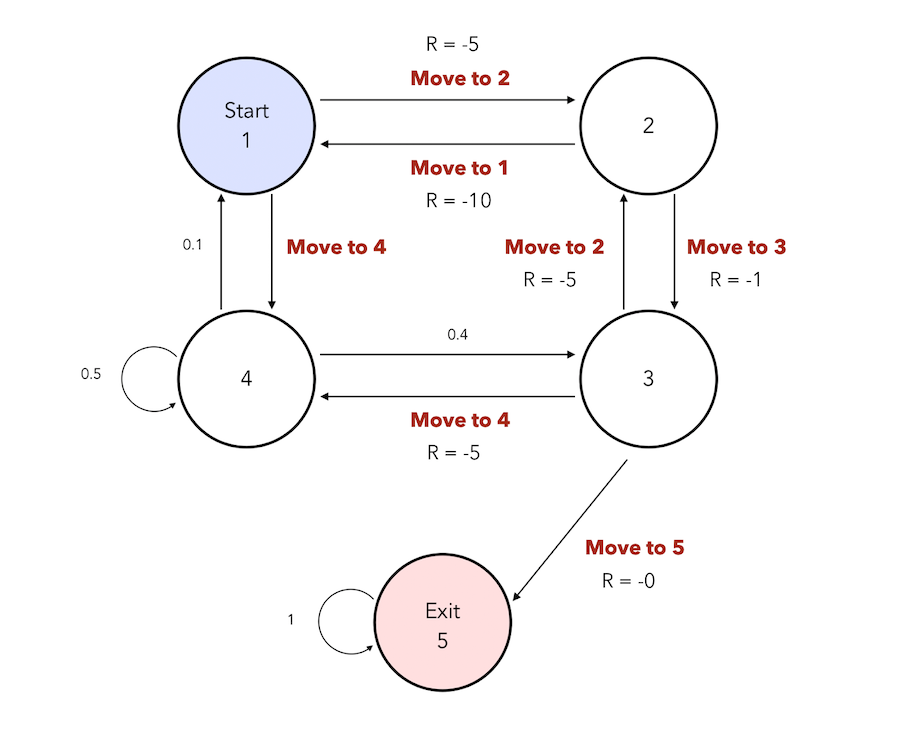
\includegraphics[width=0.8\linewidth]{figures/mdp.png}
	\caption{ (From \cite{markovdecisionprocessgithub}) Markov Decision Process with 5 states as the circles, actions are modeled with the red letters over the arrows, that represent the transition between states. When a transition is performed, a reward is returned (letter R), and a new state is achieved. We can see that there might be transitions where we cannot take an action, and we are subject to the transition probabilities (the dynamics) of the MDP.}
	\label{fig:mdp}
\end{figure} 

As we can see, the process always follows the same pattern. If we define $\mathcal{H}_t$ as the history over the MDP, we could formalize a trajectory as in equation \ref{eq:mdp_trajectory}.

\begin{equation} \label{eq:mdp_trajectory}
	\mathcal{H}_t = s_1, a_1, r_2, s_2, a_2, r_3 ... s_{t-1}, a_{t-1}, r_t, s_t
\end{equation}

Given this sequentiality in the decision making, the objective is to map this sequence of pairs state,actions (the history) to future actions that maximize the expected reward. This approach is not always useful, since in markovian processes, the current state $s_t$, is a function of the history $\mathcal{H}_t$. A markovian state uses the maxima: "\textit{the future is independent of the past, given the present}", meaning that the current state $s_t$ is a sufficient statistic of what happened in the past and it conditions what may happen next. This is formally defined in equation \ref{past_ind_fut}, where $\mathbb{P}$ represents the probability and $|$ represents the condition of a probability distribution.

\begin{equation} \label{past_ind_fut}
	\mathbb{P}[S_{t+1} | S_t] = \mathbb{P}[S_{t+1} | S_1, ..., S_t]
\end{equation}

The agent has three major components:
\begin{itemize}
	\item \textbf{Policy}: How the agent models the picked actions given a state. It may be deterministic or stochastic, and it is usually referred as $\pi$ in the notation. For example, if the policy is deterministic then we can define a mapping, such as $\pi(s)=a$, but if the policy is stochastic, then it can be defined as a probability distribution, such as $\pi(a|s) = \mathbb{P}[A=a|S=s]$.
	\item \textbf{Value Function}: A function that models how good a state is. It models a prediction of the expected future reward. Our actions usually will be influenced by how good an outcome will be by selecting an action a, given a state s. The value function models the delayed reward principle, that states that maybe an action that has a higher short-term reward, may lead to lower rewards in the future, while a low short-term reward may lead to states with higher rewards. In future sections we will formalize this concept, giving a mathematical and analytical explanation.
	\item \textbf{Model}: Useful information that the agent picks in order to build a model of the environment to understand what it might do next. This modelling consists in estimate two already known elements: the transition probability matrix $\mathcal{P}$ and the reward function $\mathcal{R}$ from the environment. Estimations are modelled by:
	\begin{enumerate}
		\item Transition probability estimation: $\mathcal{P}_{s s'}^a = \mathbb{P}[\mathcal{S'} = s' | \mathcal{S} = s, \mathcal{A} = a]$ 
		\item Reward function estimation: $\mathcal{R}_{s}^a = \mathbb{E}[\mathcal{R} | \mathcal{S} = s, \mathcal{A} = a]$ 
	\end{enumerate}
\end{itemize}

Usually, there are two types of environment modelling: model-based and model-free. In model-free RL, the agent ignores the environment's model, since it does not need to understand how the dynamics work. Instead, it uses observations and reward to build a value function and a policy that maximizes the reward. Model-based tries to make the estimations of the environment dynamics, and use them to plan and execute policies that maximize the reward. For this work, we will mainly focus on the model-free approach.

Finally, agent categorization is an important part in the RL framework. There are two principal categories (although with recent advancements, new categories have appear in the RL scene): value-based agents and policy-based agents. We will delve into this in the following sections, but we will give a brief introduction here. Value-based methods estimate the value of states in the environment and create a function that is used by the policy in order to perform actions. If only states are taken into account to provide this value estimation given a policy $\pi$, then the notation used will be $V_{\pi}(s)$. If the information to provide a value depends on both states and actions, then, we will refer to them either by ${Q}_{\pi}(s,a)$ or ${q}_{\pi}(s,a)$. On the other hand, policy-based agents only make use of policy optimization to maximize rewards, without using the value function. This two approaches can be mixed up in a symbiotic approach, using the policy and the value function to maximize the returns. This approach is usually called actor-critic methods, where the actor is the policy and the critic is the value function.

\subsection{Value-based RL}
\label{sec:val-based-rl}
In model-free RL, we do not have any clue of the environment's dynamics. Still, proper choices need to be done in order to maximize rewards. A value function estimates how good an state is, not only for the short-term, but also for the long term. This value function is also conditioned on a given policy $\pi$, so we will define the value function as in equation \ref{eq:state_value}, where we define the episodes of experience following a policy as $S_1, A_1, R_2, ..., S_k \sim \pi$ and the returns $G_t = R_{t+1} + \gamma R_{t+2} + \gamma^2 R_{t+3} ... + \gamma^{T-1}R_{t-1}$.

\begin{equation} \label{eq:state_value}
	V_{\pi}(s) = \mathbb{E}_{\pi}[G_t | S_t = s]
\end{equation}

For various purposes, the state information may not be sufficient to estimate the value of a state itself, so the action must be part of the value associated. Formally, it is described as in equation \ref{eq:action_value} and this kind of values are formally known as action values.

\begin{equation} \label{eq:action_value}
	q_{\pi}(s,a) = \mathbb{E}_{\pi}[R_{t+1} + \gamma q_{\pi}(S_{t+1},A_{t+1}) | S_t=s , A_t=a]
\end{equation}

Usually, in model-free reinforcement learning ${Q}$-values are common approach, since with the state values, the environment dynamics $\mathcal{P}$ should be at least known or estimated. This is why in following sections, the formulation will be more focused on ${Q}$-values. Section \ref{app:on-policy-control} expands on this matter.

There are several approaches that make use of the value function definition to make estimations about it. In this section we will briefly go over Temporal Difference Learning: TD(0) and a two special cases: Deep Q-Networks (DQN) and Double Deep Q-Networks (DDQN). Again, if deeper insights are needed, we encourage the reader to take a look at section \ref{app:classic_rl} where we explain in depth several important aspects of methods like Monte Carlo learning or TD learning. Our main focus will be in the value function approximators, since this is when deep learning made its appearance in the RL framework.

\subsubsection{Value function approximation} 
\label{sec:val-fun_approx}

Environments in RL may end up being quite complex. This complexity usually comes from the number of possible states of our environment. For example, a robot walking down a street finds itself constantly in new states, as the observation of the environment changes constantly (i.e people coming by, cars running down the street... etc). Creating a table that models such a complex space may be infeasible, but we can use and optimize a high parameterized function to approximate the optimal value function, and here is where deep neural networks make their appearance. Formally, the goal of the optimization is described in equations \ref{eq:value_aprox} and \ref{eq:q_value_aprox}, where \textbf{w} is a vector that holds the weights (or parameters) from the function approximator.

\begin{equation}\label{eq:value_aprox}
	\hat{V}(s,w) \approx V_{\pi}(s)
\end{equation}

\begin{equation}\label{eq:q_value_aprox}
	\hat{q}(s,a,w) \approx q_{\pi}(s,a)
\end{equation}

In this section we are going to focus on the action value function $\hat{q}(s,a,w)$. This function approximator could be defined as the combination of the input features $\phi$ by the weights (eq. \ref{eq:comb_qval}).

\begin{equation} \label{eq:comb_qval}
	\hat{q}(s,a,w) = \phi(S,A)^T w = \sum_{j=1}^{n}\phi_{j}(S,A) w_j
\end{equation}

The objective of Value Function Approximation is similar to a supervised learning scenario. In equation \ref{eq:sgd_objective_function} it is defined to minimise the Mean Squared Error (MSE) of the difference between the objective function $q_{\pi}(s,a)$ and the approximation $\hat{q}(s,a,w)$. This optimisation is done via Stochastic Gradient Descent (SGD) (equation \ref{eq:sgd_opt}) where we derive the MSE with respect to the set of parameters w, looking for the steepest part of the curve for descending it in order to minimize the error. Since we do not have the objective function $q_{\pi}(s,a)$, we must adjust our parameters to the estimations we collect as we explore the state space.

\begin{equation} \label{eq:sgd_objective_function}
	\mathcal{J}(w) = \mathbb{E}_{\pi}[(q_{\pi}(S,A) - \hat{q}(s,a,w))^2 ]
\end{equation}

\begin{equation} \label{eq:sgd_opt}
	-\frac{1}{2} \nabla_{w} \mathcal{J}(w) = (q_{\pi}(S,A) - \hat{q}(s,a,w)) \nabla_{w}\hat{q}(s,a,w)
\end{equation}

This approach can be applied to TD learning for example. In the case of TD(0) (equation \ref{eq:value_approx_td0}), the adjustments for the weights of the function approximation $\Delta_{w}$ would be done using the difference of the information we already know $\hat{q}(s_{t},a_{t},w))$ and the new information that we have acquired with the new transition $R + \gamma \hat{q}(s_{t+1},a_{t+1},w)$. The same is done for TD($\lambda$) in equation \ref{eq:value_approx_tdlambda}.

\begin{equation} \label{eq:value_approx_td0}
	\Delta_{w} = (R + \gamma \hat{q}(s_{t+1},a_{t+1},w) - \hat{q}(s_{t},a_{t},w)) \nabla_{w}\hat{q}(s_{t+1},a_{t+1},w)
\end{equation}

\begin{equation} \label{eq:value_approx_tdlambda}
	\Delta_{w} = (q_{t}^{\lambda} + \gamma \hat{q}(s_{t+1},a_{t+1},w) - \hat{q}(s_{t},a_{t},w)) \nabla_{w}\hat{q}(s_{t+1},a_{t+1},w)
\end{equation}

One of the biggest success in the value function approximation paradigm is Deep Q-Networks (DQN) \cite{mnih2013playing} that uses Q-Networks to estimate the value function using neural network. This algorithm first produces experiences and stores them into the experience buffer $\mathcal{D} = \{(s_i, a_i, r_i, s_{i+1}, d_i)\}_{i=1}^N$, where N is the size of the buffer. Then, with an off-policy Q-leaning approach, a loss function (equation \ref{eq:dqn_loss}) is proposed. The main goal is to minimize the MSE, and, as it does, it learns a value function that produces the ${Q}$-values for each possible action.

\begin{equation} \label{eq:dqn_loss}
	\mathcal{L}_w = \mathbb{E}_{\mathcal{D} \sim s, a, r, s'} \left[ \left( r + \gamma \max_{a'} Q(s', a'; w^-) - Q(s, a; w) \right)^2 \right]
\end{equation}

\noindent where:
\begin{itemize}
	\item $Q(s, a; w)$: represents the neural network with the updated weights.
	\item $Q'(s', a'; w^-)$: represents the frozen neural network with the previous weights.
\end{itemize}

The main intuition behind this loss function resides in the offline network $Q(s', a'; w^-)$ as a force that tries to maximize reward at each possible future state s' with the weights of previous iterations $w^-$, and the online network $Q(s, a; w)$ that tries to minimize the gap of its predictions, but for the current state s. This makes the online network to update its predictions towards what the offline network is maximizing, giving a good estimate of the Q values for a given present state s and an action a. Years later, Double Deep Q-Networks (DDQN) \cite{vanhasselt2015deep} made a few updates upon DQN, achieving ever better results. The goal is to minimize the loss function presented in equation \ref{eq:ddqn_loss} 

\begin{equation} \label{eq:ddqn_loss}
	\mathcal{L}_w =  \mathbb{E}_{\mathcal{D} \sim s, a, r, s'} \left[ \left( r + \gamma Q(s', \operatorname*{argmax}_{a'} Q(s', a'; w); w^-) - Q(s, a; w) \right)^2 \right]
\end{equation}

The motivation behind this update mainly reside in the fact that DQN overestimates the Q-values, which bias the agent into thinking that some state are more valuable that what they really are. This is because in the DQN loss, the action selection is done by maximizing the estimates of the target network, but, since we are trying to evaluate how good the online network is doing, it makes more sense that the action evaluated by the target network is selected by the online network, which gives us a better idea of how the agent is performing since the online network is the one used on the behaviour policy.

\subsection{Policy-based RL}
\label{sec:pol-grad-ac}
In the value based methods, the policy usually is deterministic. In section \ref{app:on_policy_control}, we go deeper in exploring greedy and $\epsilon$-greedy policies as a mapping from state/action value functions to actions, but the main important take, is that deterministic policies are not always enough for some complex environments. We can make use of parameterization in order to make our agent more capable of dealing with harder problems expanding the representation capabilities for decision making. A good policy usually is the one that maximizes the reward in each time-step, so we must always look in the direction that provides greater expected rewards using action selection. 

\subsubsection{Policy Gradient Theorem}
\label{sec:pol-grad-theorem}
The parametrized policy is defined as in equation \ref{eq:param_policy}. Where $\theta$ is the parameter vector of our function approximator (i.e. a neural network).
\begin{equation} \label{eq:param_policy}
	\pi(a|s, \theta) = \mathbb{P}[a|s, \theta]
\end{equation}

These parameters must converge to a solution where our policy maximizes the rewards, taking actions that consequently do so. The policy gradient theorem states that in order to obtain the optimal policy $\pi^*(a|s, \theta)$ that maximizes the rewards, we must compute the gradient defined in equation \ref{eq:policy_gradient_theorem}
\begin{equation} \label{eq:policy_gradient_theorem}
	\nabla_{\theta}\mathcal{J}(\theta) = \mathbb{E}[\nabla_{\theta} log (\pi_{\theta}(s,a)) {Q}^{\pi_{\theta}}(s,a)]
\end{equation}

Where the term $\nabla_{\theta} log (\pi_{\theta}(s,a))$ gives us a likelihood estimation of how much does the agent want to be in the same state and action pair. If the reward is big, we want that gradient to be big, and follow that direction, using Stochastic Gradient Ascend (SGA). On the other hand, the term ${Q}^{\pi_{\theta}}(s,a)$ measures how beneficial was taking the action a. It ponders the direction of the gradient we want to maximize. If we had a situation of great value, then that gradient should be explored more, hence the bigger values, but, if the gradient or the value is low, the agent should not be in that position very often, to avoid loss of potential reward.

One of the first policy gradients method is REINFORCE. It is based in the Monte Carlo learning method. Here ${Q}^{\pi_{\theta}}(s,a) = v_t$, where $v_t$ is the cumulative expected reward for time-step t. The weight updates are done as defined in equation \ref{eq:reinforce}, where t is the current time-step. For further reading, more in depth detail about different policy gradients methods such as Actor-Critic (A2C) is discussed in section \ref{sec:ac-methods}.

\begin{equation}\label{eq:reinforce}
	\Delta\theta_{t} = \alpha(\nabla_{\theta} log \pi_{\theta}(s,a)v_t)
\end{equation}

\section{Attention-based models}
\label{sec:attention}

\subsection{What is attention?}
\label{sec:whats-attention}
The attention mechanism was first introduced in \cite{bahdanau2016neural}. There, the authors explain how difficult is to make translations from different languages. The issue in particular was the alignment, meaning that the number of tokens or words in a translated sentence usually is different compared to said sentence in the original language. This presented a challenge for the network since it had to detect which parts of the original sentence produced the resulting translation at token level. For example, the word "crosswalk" in English, translates to Spanish as "paso de peatones" which is not a literal translation. Therefore, the task presented in this particular example would be to teach the network to align a single word in English to the counterpart three words in Spanish. We encourage the reader to go to section \ref{app:attention-mec} for further reading on the details of the attention mechanism.

The authors tackled this problem by using an recurrent encoder-decoder architecture using recurrent neural networks (RNNs) as presented in figure \ref{fig:alignmentattention}, extracted from \cite{understandingattentionmechanism}. The encoder is based on an Bidirectional Long-Short-Term-Memory (Bi-LSTM) network, that takes the token embeddings from the input, and process them creating the vector $h_j$, which contains all the information from the input up to time-step $j$. The decoder is another RNN network that has as input a context vector $c_i$ and maps it to a hidden state vector $s_i$ and an output vector $y_i$, where $i$ is the time-step of to the output. The context vector $c_i$ is obtained by pondering the embeddings produced by the encoder using vector $\alpha_i$. 

\begin{figure}[!h]
	\centering
	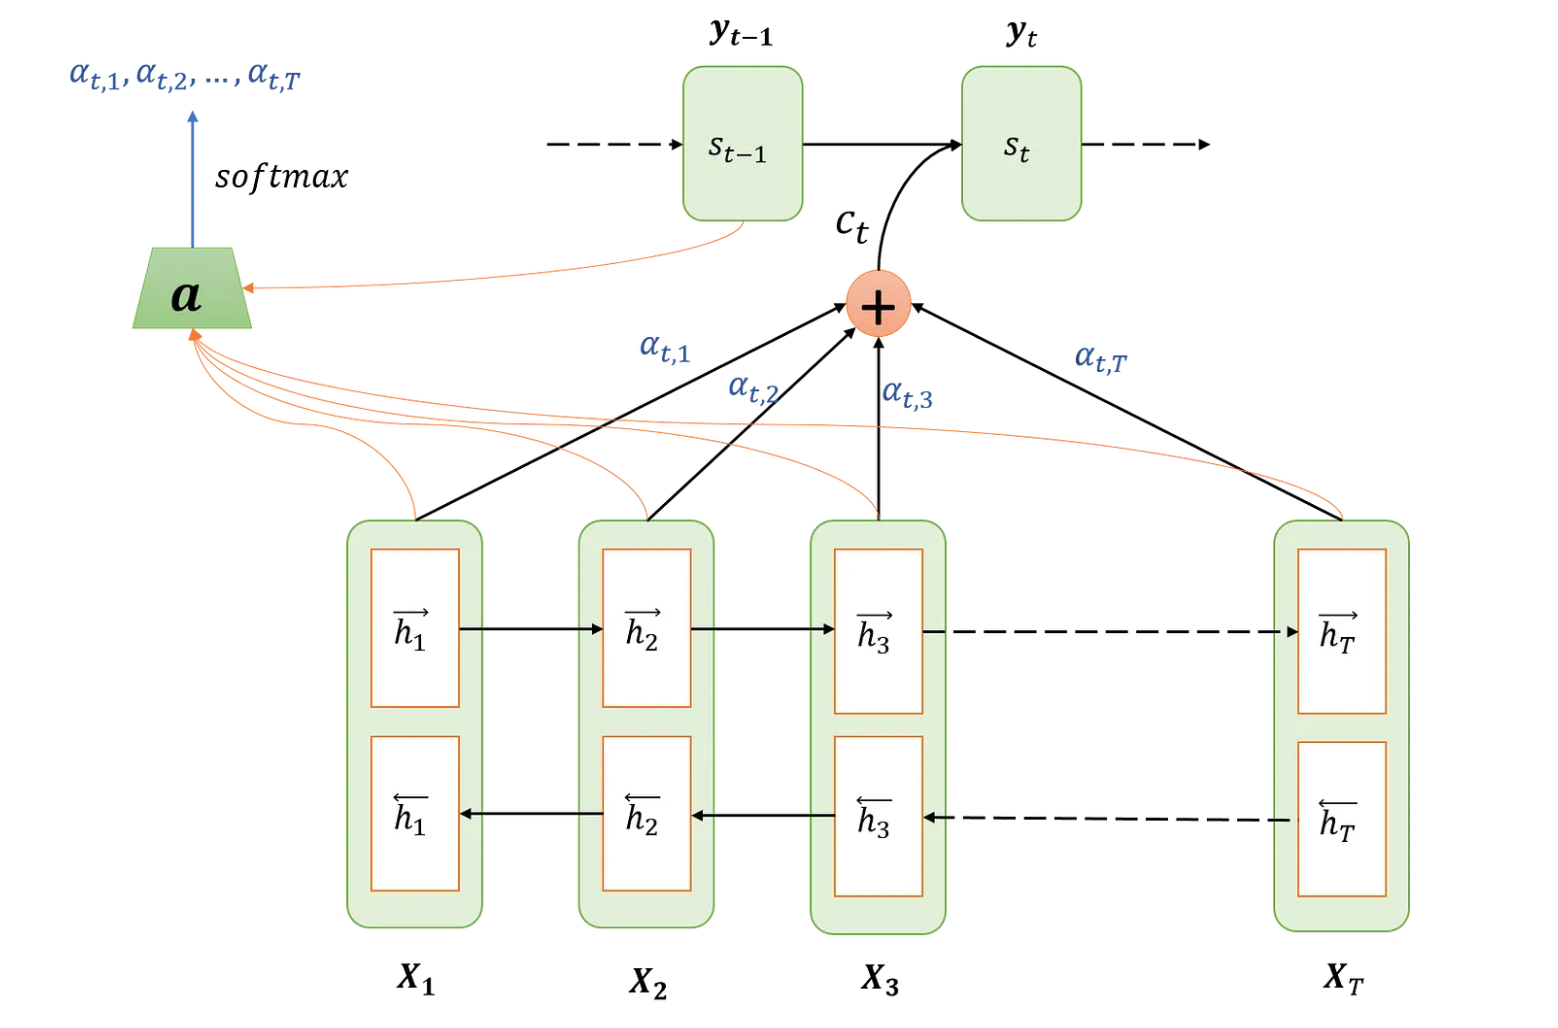
\includegraphics[width=0.7\linewidth]{figures/alignment_attention}
	\caption{Aligning inputs using the attention mechanism. First, the inputs $X_1, X_2, X_3, ... X_{\tau}$ are encoded using a bi-directional RNN, obtaining the embeddings $\protect\overrightarrow{h} , \protect\overleftarrow{h}$. This embeddings are then pondered by the product of the learnable parameters $\alpha_{i \tau}$ for each input, creating the context vector $c_t$. Finally, $c_t$ is fed into the decoder, updating the hidden state $s_t$ and producing the output $y_t$.}
	\label{fig:alignmentattention}
\end{figure}


\subsection{The Transformer Architecture}
\label{sec:transformer}

The architecture introduced in section \ref{sec:whats-attention} had its limitations, especially in modelling dependencies between sections of the input text that were far apart. This was because the fixed compressed representation (the embedding) of the input of the decoder only holds information from the closest tokens, not being able to model long-range dependencies. To tackle this problem the Transformer architecture  \cite{vaswani2023attention} introduced self-attention, where the whole sequence is processed at once and the dependencies are computed altogether, instead of processing the inputs one per time-step. Self-attention is defined as in equation \ref{eq:attn_eq}, where Q, K, and V represent the query, key, and value matrices, respectively, $d_k$ represents the dimensionality of the keys and queries, $\sigma$ represents the soft-max function applied along the rows of the matrix resulting from the dot product of Q and $K^T$. This creates a vector of weights that ponder the importance of each element of the input with respect to the rest of the elements, describing how relevant are for the model. Finally, this weights are multiplied element-wise with the value matrix V to compute the final attention output. We can think about the query (Q) as a vector that holds information about what each token in the input is looking for, meaning, which other tokens is interested in. On the other side, the keys (K) represent the information each token from the input holds. When transforming the input onto the query-value space, vectors (embeddings) that are close will have a higher dot product result, meaning that the "energy" of their semantic relation is bigger. On the other hand, if those vectors are quite far, the dot product will be smaller, hence, the energy will be lower, meaning that those vectors are not quite related. The implications that this work had in the AI research field were huge, and it was in part, because it, revealed a new upcoming discovery for explainability in neural networks, thanks to the weights the attention matrix holds

\begin{equation} \label{eq:attn_eq}
	\text{Attention}(Q,K,V) = \text{$\sigma$}\left(\frac{QK^T}{\sqrt{d_k}}\right)V
\end{equation}

What we have explained up until now it is know as an attention "head", this means that there is only one participant looking for relevant information in a sequence, but, it is well known that having several model instances cooperating to solve a problem is always better \cite{model_emsembling_survey}. In order for the attention mechanism to look at different parts of the inputs at the same time, we need multiple instances looking at different parts and communicating between them. This is known as Multi-Head Self Attention (MHSA). When we have multiple attention heads \cite{vaswani2023attention}, we can extract a rich feature map that ponders the important of different parts of information from the input. Because multiple heads can focus on different parts of the input, our attention maps will be quite diverse, preventing over-fitting. This approach also takes advantage of distributed computation, because computing the self-attention for each attention head can be done in parallel, making it efficient in time. Figure \ref{fig:multihead_attn} provides a diagram that explains the very same concept discussed in this section.

\begin{figure}[!h]
	\centering
	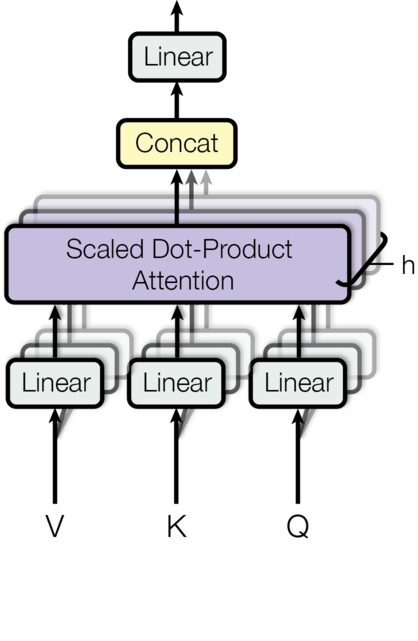
\includegraphics[width=0.25\linewidth]{figures/multi_head_attn.png}
	\caption{Multi-head attention. The embeddings from Q, K and V are computed and fed into the attention module. Once computed, the attention matrix is computed for each of the heads, and concatenated to then, be forwarded onto a linear layer, that computes the embedding of the attention-weighted input.}
	\label{fig:multihead_attn}
\end{figure} 

In figure \ref{fig:transformer_arch}, we can see the complete transformer architecture. First we can the encoder, that uses attention to generate the embeddings of the sequence, where in each time step, the attention heads will focus in different parts of the input. Then, the decoder takes those embeddings and starts producing the outputs in an auto-regressive manner, taking its own outputs as input embeddings to the decoder that are mixed with the embeddings of the encoder, to provide a wider context of the whole sequence.

\begin{figure}[!h] 
	\centering
	\subfloat[Transformer architecture.]{%
		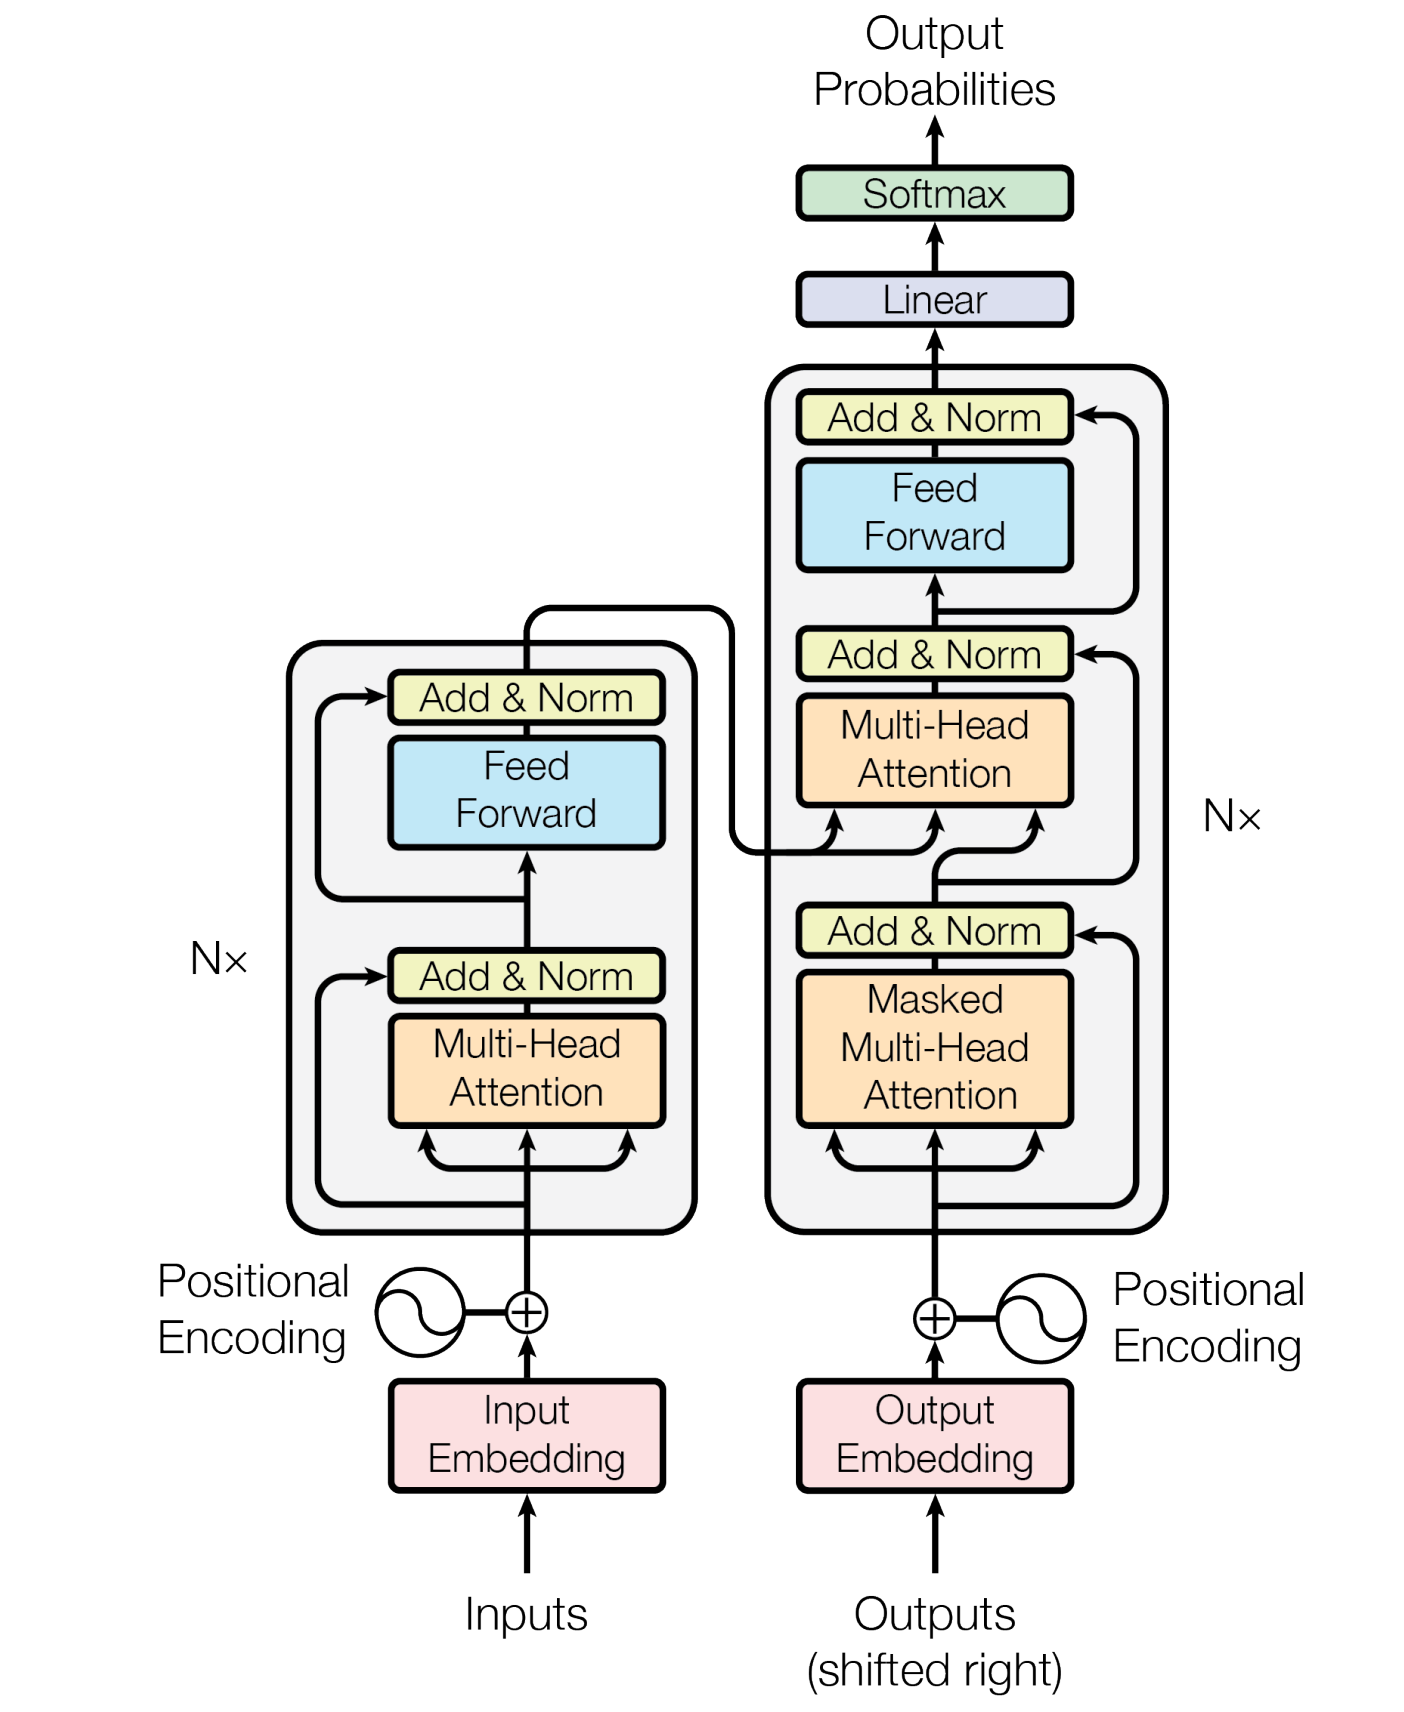
\includegraphics[width=0.5\linewidth]{figures/transformer_architecture.png}%
		\label{fig:transformer_arch}%
	}%
	\hfill%
	\subfloat[Cross-Attention weights for the translation task]{%
		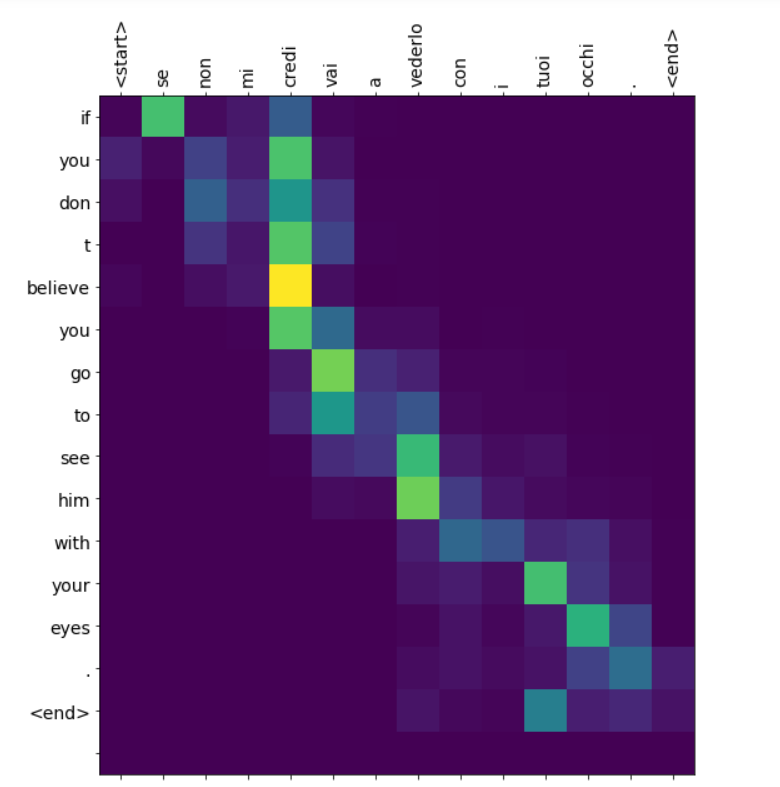
\includegraphics[width=0.5\linewidth]{figures/text_translation_attn.png}%
		\label{fig:translation_attn}%
	}%
	\caption{In figure \ref{fig:transformer_arch} (left), from \cite{vaswani2023attention}, the complete transformer architecture is presented. In figure \ref{fig:translation_attn} (right) from \cite{translationmin2023attention}, an attention matrix is presented for a sentence and its translated counter-part. The weights for each word quantify how much \textit{attention} is the model paying to the words from the original sentence in order to produce the translation to the new sentence.}
\end{figure}


Naturally, one can see the attention weights are the main piece of information that explains the output. Attention weights provide a numerical description of which parts of the input the algorithm is looking for, thus providing an approximate explanation of the output. In figure \ref{fig:translation_attn} we have an example of how a transformer performs translation between English and Portuguese, providing the correct alignments for each word. 

\subsection{Vision Transformers}
\label{sec:vis-transformers}
Self-attention is a powerful mechanism, that can be applied not only to sequences, but also to visual data. The vision transformer (ViT) \cite{vit} was one of the first models that leveraged the self-attention mechanism in order to process images. The architecture is presented in figure \ref{fig:vit_arch}, where the first thing to notice is that there is only an encoder in the architecture. This is because this model was designed for image classification, and the best approach to solve this task is to extract an embedding as a compressed representation of the original image. The input is processed by patching the image, creating different blocks that serve as input. To take context of which patch is in which position of the image, the ViT model has a learnable parameter that serves as an absolute positional embedding. Then, the attention heads will look at each of the patches separately. To do this, the ViT flattens the patches from the images and treats it as a sequence, paying attention to the features from the raw input that are more relevant. By having several attention heads looking at several patches at the same time, the model captures global dependencies between them, obtaining a rich representation of the image. After that, the attention matrix computed from each head is concatenated and forwarded into a multi-layer perceptron (MLP) that produces the embedding that the classifier will use to produce the output.

\begin{figure}[!h] 
	\centering
	\subfloat[Transformer architecture.]{%
		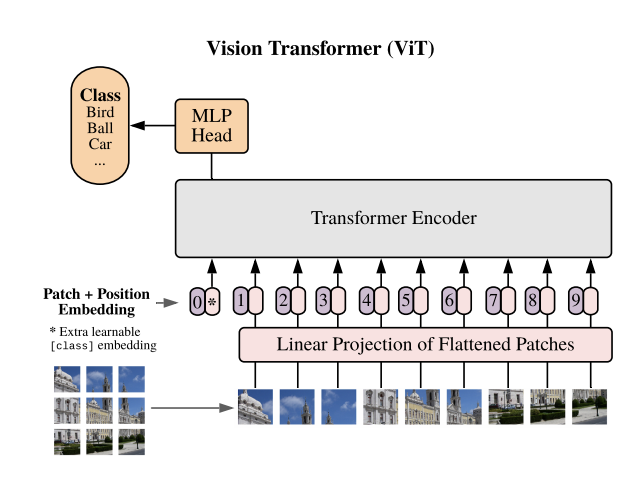
\includegraphics[width=0.5\linewidth]{figures/vision_transformer.png}%
		\label{fig:vit_arch}%
	}%
	\hfill%
	\subfloat[Attention weights for human detection task]{%
		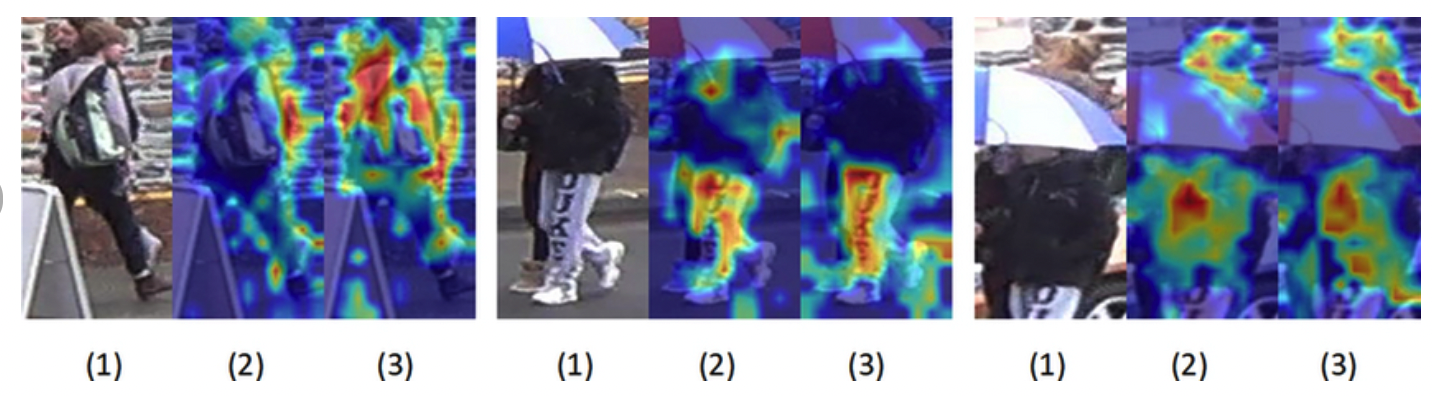
\includegraphics[width=0.5\linewidth]{figures/visual_attention_occlusion.png}%
		\label{fig:attn_maps}%
	}%
	\caption{In figure \ref{fig:transformer_arch} (left) the ViT transformer architecture is presented. In figure \ref{fig:translation_attn} (right) an attention map is presented. The model that produced the attention maps was trained to track people on a scene, and it is why, the higher attention weights (red) are put in the pixels where people is present.}
\end{figure}


\subsection{SWIN Transformer}
\label{sec:swin-transformer}
One of the main issues that the ViT model holds, is the computational cost of the self-attention module being quadratic. This means that, as images are bigger, the number of patches where the attention is performed will increase, making the input embeddings more expensive to process. To solve this, the SWIN Transformer \cite{liu2021swin} (figure \ref{fig:swin_transformer_parts}) takes an alternative approach, and uses a hierarchical architecture that resembles the CNNs. First, it divides the image in patches, as the ViT model does, but, instead of computing the attention, it adds the concept of window attention to the mix. A window will contain a set of patches, and the attention will be performed between the patches that are inside the window. This reduces the complexity of the attention operation, but at the cost of global feature extraction, since the patches inside of a window only know the existence of themselves, but not of their neighbours under a different window. To solve this, the SWIN Transformer introduces masked window shifting and patch merging. 


\begin{figure}[htbp]
	\centering
	\begin{subfigure}{0.28\textwidth}
		\centering
		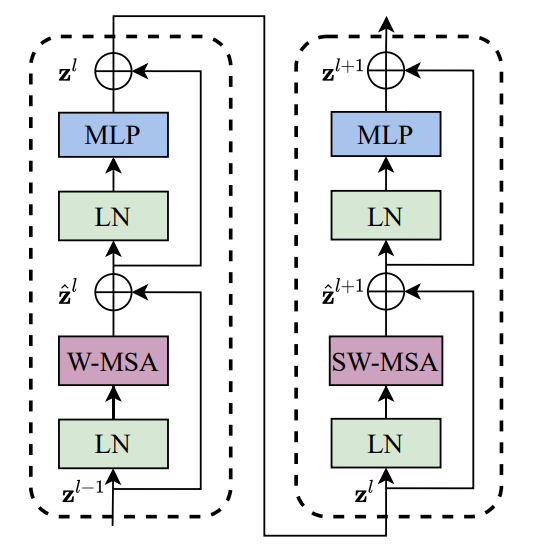
\includegraphics[width=\textwidth]{figures/swin_blocks}
		\caption{Swin Transformer block}
		\label{fig:swinblocks}
	\end{subfigure}
	\begin{subfigure}{0.7\textwidth}
		\centering
		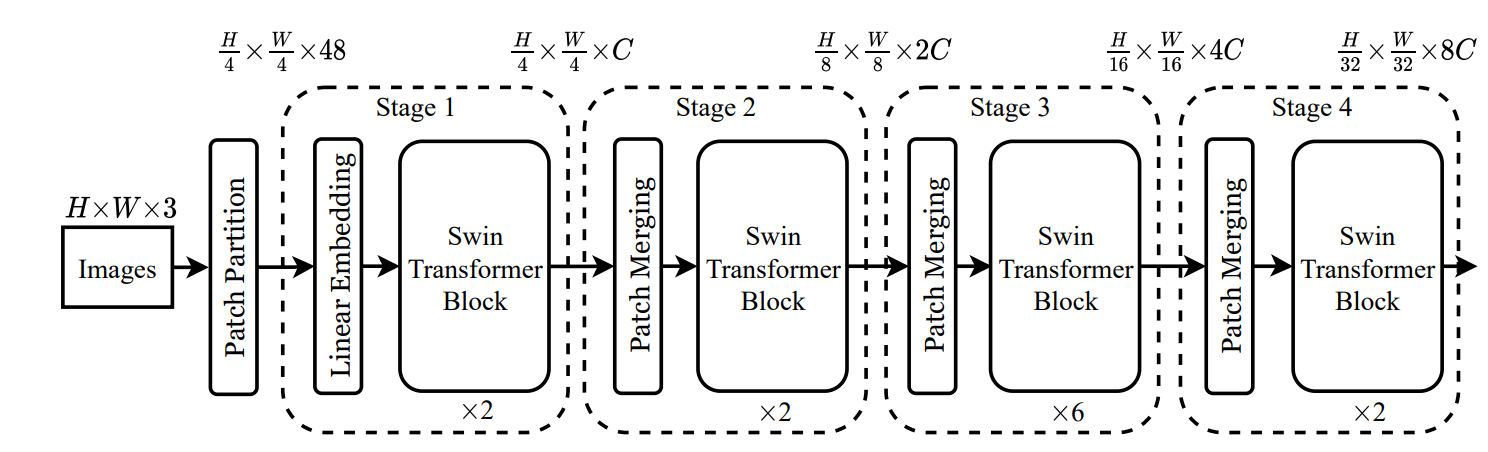
\includegraphics[width=\textwidth]{figures/swin_architecture}
		\caption{SWIN Transformer architecture}
		\label{fig:swinarchitecture}
	\end{subfigure}
	\caption{Swin Transformer architecture and its building blocks. The transformer block, figure \ref{fig:swinblocks}, has two phases. In the first one (left-most block), it performs a layer normalization, followed by a window-MSHA block that is forwarded onto a MLP with a neurons ratio of 4. In the second, it makes use of the shifted window MSHA, instead of the window-MHSA. In figure \ref{fig:swinarchitecture} we can see the whole SWIN Transformer architecture, where each of the "stages" are built upon the transformer blocks, that have as input the patch merged embeddings that are passed at each stage.}
	\label{fig:swin_transformer_parts}
\end{figure}

Masked window shifting, presented in figure \ref{fig:windowshifting} is a simple but effective procedure to broaden the spatial context of the windowed attention. The intuition is to drift the layout of the patches inside the image, providing a wider spatial context to the attention performed inside the windows. This means that the group of patches that are left out of the image (sections A, B, C) are mirrored to the symmetric part of the image, performing a \textit{"cyclic shift"}. This cyclic shift alters the spatial disposition of the elements in an image, since the parts of the top left are now in the bottom right. To handle this, they provide a mask that ensures that the shifted regions only attend to their corresponding parts. For example, the patches inside region A will only attend to patches that are only inside said, region. This ensures that the spatial information remains unaltered and no "abnormal" representations are learn as a product of this shifting. 

On the other side Patch Merging, figure \ref{fig:patchmerging}, is an operation that uses concatenation along the channel dimension to aggregate the features from the patches inside a window. This provides a hierarchical architecture, where the local features are captured in the first stages of the architecture, since the spatial dimension is bigger, and the global features are captured at the latest stages, where the spatial dimension is diminished, and all the local features are aggregated along the channel dimension. The patches are selected in a 2 by 2 grid, so the input has a shape of $W \times H \times C$, and after the patch merging, has a shape of $\frac{W}{2} \times \frac{H}{2} \times 4C$. In some type of way, this could be seen as a \textit{"convolutional transformer"}, since it quite resembles some of the hierarchical mechanisms that the CNNs have to perform feature extraction from an image. 

\begin{figure}[!h]
	\centering
	\begin{subfigure}{\textwidth}
		\centering
		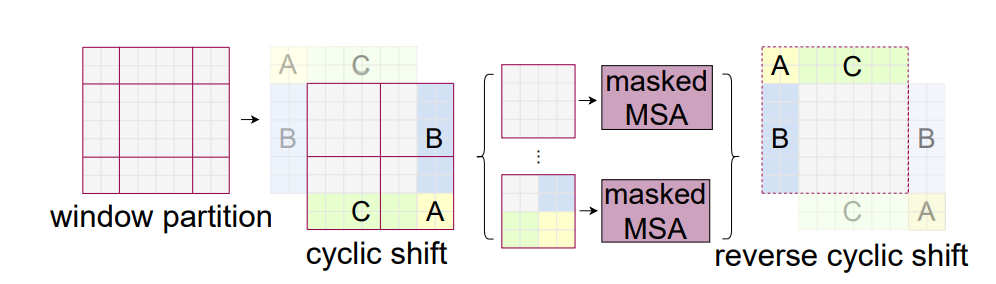
\includegraphics[width=0.8\linewidth]{figures/windowshifting}
		\caption{Window shifting and cyclic shifting module}
		\label{fig:windowshifting}
	\end{subfigure}
	\hfill
	\begin{subfigure}{\textwidth}
		\centering
		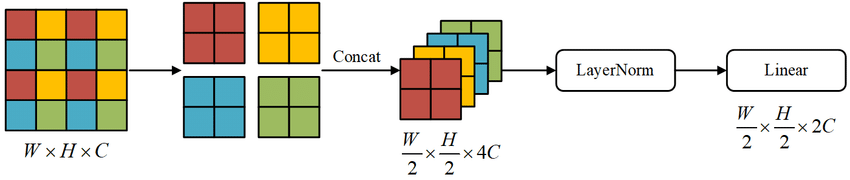
\includegraphics[width=0.9\linewidth]{figures/patch_merging}
		\caption{Patch merging module for hierarchical feature aggregation (image from\cite{swin_unet})}
		\label{fig:patchmerging}
	\end{subfigure}
	\caption{Window shifting in the SWIN Transformer architecture (figure \ref{fig:windowshifting}). From the window partition, shift to the bottom right, so the A, B, C patches are rearranged in the mirrored side of the image. Patch Merging (figure \ref{fig:patchmerging}), picks blocks of 2 by 2 patches inside a window and concatenates them along the channel dimension.}
	\label{fig:combined}
\end{figure}

\section{Explainable AI}
Explainable AI (XAI) refers to techniques and methods that make the behavior and decisions of artificial intelligence systems transparent, understandable, and interpretable to humans. It aims to clarify how AI models reach their conclusions, enhancing trust, accountability, and usability, especially in critical applications like healthcare and finance. The concept of explainable AI has been around for quite some time. In the eighties, in \cite{swartout1985explaining}, Swartout explains that the need for systems that have "cognitive" abilities to solve complex problems must come with an explanation, and developed a basic rule-system to explain the results. It is clear that, since the AI research began, researchers have always claimed the need for mechanisms and systems to explain decision making. There are some AI models that are quite good at, this, like decision trees, since is quite common to follow down the nodes and leaves (questions and conditions that the tree proposes in order to perform inter-class separability) in order to understand the decisions performed to classify a given input with a certain class, presenting a reasoning of a final decision. The issue comes when the complexity of the model increases. For example, a random forest is a set of decision trees that jointly participate in a poll to determine, the class of a given input. The set of decision trees can be huge for complex datasets, and to trace each and everyone of the decisions performed by all of the trees can be an exhaustive process. Something similar happens with deep neural networks. With the appearance of AlexNet \cite{alexNet} in the ImageNet challenge \cite{ILSVRC15}, a shift of paradigm appeared, since the following years, deeper models were presented to the challenge. Results at the time were astonishing, but with a cost, since as the network got deeper, the interpretation of the activation maps in the receptive fields of the layer was almost impossible, which led to a big concern: what is the network looking at in order to make the predictions? One thing is clear, as shown in Figure \ref{fig:explainablechart} from \cite{Turek2017}, the accuracy is higher when less explainable is the model.

\begin{figure}[!h]
	\centering
	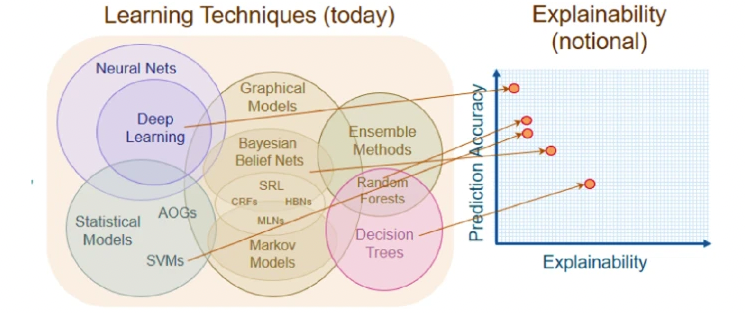
\includegraphics[width=0.7\linewidth]{figures/explainable_chart}
	\caption{Explainability of ML models against the prediction accuracy.}
	\label{fig:explainablechart}
\end{figure}

in the past decade, the field of computer vision has been involved a pursuit to make DNNs transparent and understandable. In the following sub-sections we will briefly explain the techniques that have been used in this work along with another relevant works from the XAI field.

\subsubsection{Sensitive Analysis}

In \cite{xai_survey2019, sensitivity_analysis}, sensitive Analysis (SA) is defined as a method that identifies which parts of the input are more sensitive to the network to perform the predictions. To do so, it assumes that the most relevant input features are the most sensitive for the output, and by "obstructing" pixels or sections of the image, it ponders how relevant are different sections to the predicted output. The mathematical definition behind this concept is defined in equation \ref{eq:grad_sensanalysis}, where they define all the partial derivatives for a function $f(x)$ as the sensitivity $s_{ik}$ of the network to a certain input $x_n$ with respect to all the i-th elements of the input $x_i$ and the output $y_k$.

\begin{equation}
	\label{eq:grad_sensanalysis}
	s_{ik} \bigg|_{\mathbf{x}_n} = \frac{\partial y_k}{\partial x_i} (\mathbf{x}_n)
\end{equation}

The issue that appears with SA is that it does not explain the function approximation performed by the neural network, but only quantifies the importance of the input. This may not be ideal, as we want to understand what the network gives more importance to with respect to the features of the input, not understand which parts of the network are essential to produce the output.

\subsubsection{Layer-wise Relevance Propagation}
Layer-wise Relevance Propagation (LRP) \cite{bach2015pixel} is an interpretability method used to explain the predictions of neural networks. The main idea of LRP is to propagate the prediction score $f(x)$ backwards through the network layers, assigning relevance scores $R_i$ to each neuron in the network.

There are several variations of LRP to interpret neural network predictions, but one of the most useful ones is the LRP-$\alpha\beta$, which ponders between the positive and negative contributions to the prediction, given an input. The relevance $R_i$ of each neuron $i$ is traced back layer by layer, indicating the contribution of each neuron to the final prediction. To distinguish between positive and negative contributions, LRP decomposes the term $Z_{ij} = a_i^{(l-1)} \cdot w_{ij}$, where $a_i^{(l-1)}$ is the activation of neuron $i$ and $w_{ij}$ is the weight connecting neuron $i$ to neuron $j$. The positive and negative parts are defined as $z^+_{ij} = \text{max}(0, z_{ij})$ and $z^-_{ij} = \text{min}(0, z_{ij})$. The  LRP-$\alpha\beta$ then, combines these parts to propagate the relevance from the current layer $l$ to the previous $l-1$, as defined in equation \ref{eq:lrp_alphabeta}

\begin{equation}
	\label{eq:lrp_alphabeta}
	R_i^{(l-1)} = \sum_j \left( \alpha \frac{z_{ij}^+}{\sum_{i'} z_{i'j}^+} R_j^{(l)} - \beta \frac{z_{ij}^-}{\sum_{i'} z_{i'j}^-} R_j^{(l)} \right)
\end{equation}


\subsubsection{Class Activation Maps}
\label{sec:cam}
Another widely-known approach for explainability is called class activation maps (CAM). Introduced in \cite{zhou2015learning}, the main intuition behind this technique is to use the activation units of the last layers, specially the Global Average Pooling to understand which sections of the input image generates relevant information for the final softmax layer. It is formally defined in equation \ref{eq:cam_basic}, where $M_c(x,y)$ refers to the activation for the $x,y$ pixels in the input space, given the class $c$, $w_k^c$ refers to the weights that go from the input neuron $k$ (the channel) to the output space $c$, and $f_k(x,y)$ refers to the unit $k$ in the last convolutional layer, given the input at coordinates $x,y$ of the image.

\begin{equation}
	\label{eq:cam_basic}
	M_c(x,y) = \sum_{k} w_k^c  \cdot f_k(x,y)
\end{equation}

An extension to this work is developed in \cite{Selvaraju_2019} called Grad-CAM. They use the gradients of the output with respect to the activations to compute the activations of the network under a desired class $c$. First, 
The input image $\mathbf{I}$ is passed through the CNN to obtain the feature maps from the last convolutional layer, denoted as $A^k$, where $k$ is the channel index. The network also produces a prediction score $y^c$ for each class $c$. To compute Grad-CAM, we need the gradient of the score for the target class $y^c$ with respect to the feature maps $A^k$:
\[
\frac{\partial y^c}{\partial A^k}
\]

This gradient indicates the importance of each pixel in the feature maps $A^k$ for the target class $c$. Said gradients are globally averaged over the width and height dimensions to obtain the weights $\alpha_k$:
\[
\alpha_k = \frac{1}{Z} \sum_i \sum_j \frac{\partial y^c}{\partial A_{ij}^k}
\]
where $Z$ is the number of pixels in the feature map ($Z = H \times W$) which serves as a normalization term, and $A_{ij}^k$ is the value at position $(i, j)$ in the $k$-th feature map. The operation of the global average pooling seems to perform better empirically, according to \cite{Selvaraju_2019}. To properly ponder the activations, the weights $\alpha_k$ are used to compute a weighted sum of the feature maps:
\[
L_{\text{Grad-CAM}}^c = \text{ReLU} \left( \sum_k \alpha_k A^k \right)
\]
Additionally, the ReLU function is applied to the activations in order to obtain only the positive contributions that "help" the gradient to find the most relevant regions from the input. 

The results that Grad-CAM provides are coarse, since we are generally focusing in the last layers of the network, where the spatial information is limited. To overcome this, $L_{\text{Grad-CAM}}^c$ is up-sampled to the size of the input image using interpolation methods.


\section{Reinforcement Learning using Transformers}
\label{sec:rl-with-attention}

Recently, there has been a trend into fitting the Transformer model into the RL problem. The motivation behind this resides in their quality in feature representation extraction, and, given the nature of RL and function approximation, it is natural to leverage these models abilities to try to solve the RL problem \cite{rl_transformers2023survey}. In the case of the ViT model in \cite{vit_q_learning_sample_eff} they use a Q-learning set-up in order to test wether the feature representation that provide the ViT is compatible with sample efficiency, which is a great concern in the RL field, since neural networks are known as "data-hungry" models. And, even though results are not state of the art, this work provides an alternative framework for the RL problem. Altough the ViT is not widely used in the RL paradigm, we argue that with a proper set-up it can lead to interesting findings in RL.

Swin Transformers have also been used to perform DDQN Learning \cite{meng2024deep}. Using a similar approach to \cite{vanhasselt2015deep}, they use a SWIN Transformer as a $Q$-value function approximator. As we mentioned in section \ref{sec:swin-transformer}, the ViT transformer has a quadratic cost in terms of computing the self-attention mechanism, and since DQN-learning is a sample intensive task, researchers opted to use a less computational expensive model to try to solve the problem of RL. Results in the Arcade Learning Environment (ALE) \cite{Bellemare_2013} set-up are state of the art in several games, but little is explored about the how the attention mechanism influences the decision making of the agent.

Also, we think is worth mentioning other approaches that have been proposed to solve RL using transformers. In \cite{janner2021offline}, they try to model RL as a big sequence prediction problem in an offline RL set-up, where the next action is conditioned in the past actions and reward, thus expanding the MDP approach. Right after, in \cite{chen2021decision} they introduced the decision transformer, a similar model that is focused in predict the action that maximizes the reward based only in collected experiences from previous, online trained agents, but also in an offline set-up. There has been also several intents of learn-on-the-run transformer-based set ups. For example, in \cite{wang2022bootstrapped}, they propose the bootstrapping transformer, a model that generates its own trajectories and learns from them, highly boosting the sequence offline training procedure.


\section{Explainable RL using Attention}
Explainable RL or (XRL) is a field of study that aims to understand and to provide tools that improve a RL agent explainability of their decision making.
We as humans, can explain most of the times why me take decisions or perform actions, enabling other humans to understand our behaviour. The same should happen with autonomous systems, so when implemented in industry related environments such as factories, vehicles or bots, we can understand why an agent took a decision or performed an action.

Literature in explainability for attention based architectures in RL is scarce, although some interesting proposals can be found. In \cite{BRAMLAGE202210}, they propose a attention-weighted reinforcement learning approach. They use as inspiration \cite{LEONG2017451}, where Yuan Chang Leong et al. proposed a series of tasks in order to evaluate which parts do humans pay more attention to solve them. They argue that humans attention can be approached as a hierarchical system where, as we gain knowledge from general features, the attention provides contextual information, coding the essential parts and leaving out the less relevant ones. In order to model this, they propose a value function that takes into account stimuli from multi-dimensional features to then generate a value as a numerical signal associated them. They weight the values from said features depending on the attention that subjects pays to them. In \cite{BRAMLAGE202210}, they model this relations using self-attention, with promising results when correlating features with the attention maps in tasks that involve playing games in the ALE Atari 2600 environment, but this comes with a condition. Their set-up assumes prior knowledge about several positions of elements in the environment, such as the ball coordinates or other players/enemies position in the board, conditioning the learning process, especially in set-ups where observations are visual cues. We argue that using attention-based models that show which parts are they paying attention the most, we could obtain better explanations on the visual cues taken into account to perform a decision.
			% incluir capítulo de estado del arte/state-of-art
%%%%%%%%%%%% DISEÑO Y DESARROLLO / DESIGN & IMPLEMENTATION CHAPTER %%%%%%%%%%%%%%%%%%%%%%%%%%%%%%%%%%%%%%%%%%%
\chapter{Design and development}
\label{cha:design-development}
As previously explained, one of the main differences in the RL paradigm is how the agent acquires data. Opposite to the datasets or databases in the supervised learning environment, where we have an input and a ground truth structured in such a way that the model can learn from the data adjusting itself to the ground truth, here, the data is obtained via observations from an environment, that are associated with a reward and a observation of the next state. On the other hand, we have to create a seamless pipeline for a deep neural network model that interacts with this environment and learns from it using two different off-policy algorithms: DQN and DDQN.

In this section we will explain step by step how we implemented this framework, from the environment instantiation, the post-processing of the observations provided by the environment, how we modelled the interactions of the agent over the environment and which tools we used for the memory replay module of the several agents that we developed. Additionally, we will also explain how we fitted deep learning, and especially transformers into this problem, and which modifications we developed over the original designs of these models to adapt them to the RL problem.

\section{Farama's gymnasium library}
The Farama's gymnasium (Figure \ref{fig:faramas-gym}) library was originally developed and released by OpenAI and was a huge leap in the RL realm, since before this, researchers had to develop their own environments or games to test their agents. Using games is a great way to test if an agent is actually learning from an environment, and one of the first frameworks that showed this was the Arcade Learning Environment or ALE \cite{Bellemare_2013}, where Bellemare \textit{et al.} proposed a platform with different games that were originally developed for the Atari 2600 console. ALE was quite impactful, since lots of relevant works have benefited from this platform to test and launch their agents, providing a kind of benchmark. The ALE environment was included in the Farama's gym, along with other platforms such as Multi-Joint dynamics with Contact (MuJoCo), a physics engine that test an agents ability to perform control over complex robotic entities (Figure \ref{fig:ant}) or Box2D, a platform that involve toy games in order to perform control on several vehicles, such as space-ships or cars (Figure \ref{fig:landing}).

This library will be our starting point. A deep understanding in how it works is crucial for a efficient and insightful development of our deep learning-based agents.

\begin{figure}[!h] 
	\centering
	\subfloat[Gym landing environment.]{%
		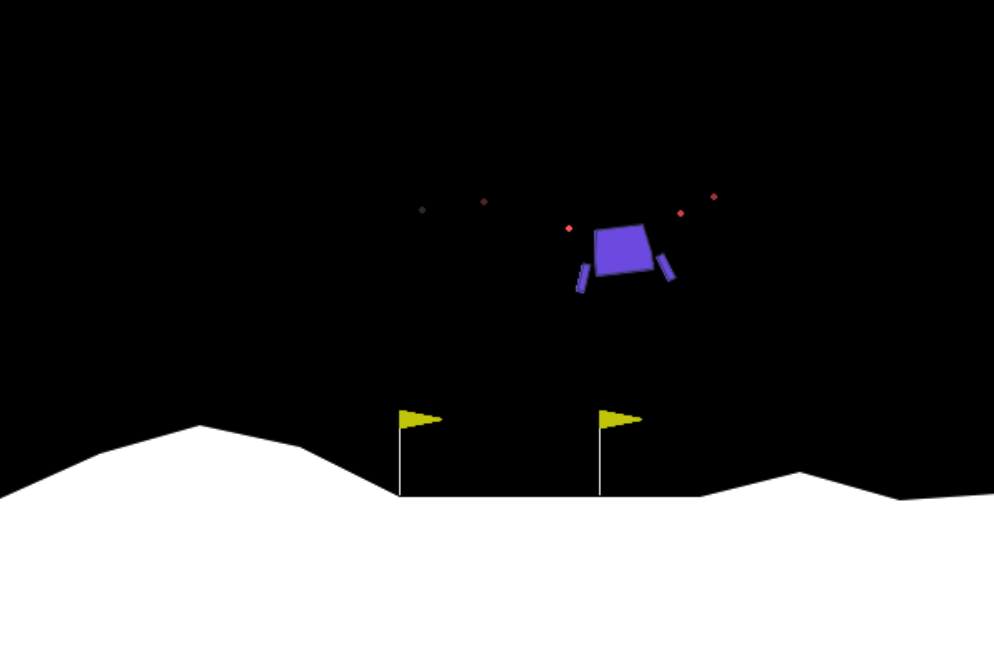
\includegraphics[width=0.45\linewidth]{figures/gym_landing.png}%
		\label{fig:landing}%
	}%
	\hfill%
	\subfloat[Ant MuJoCo environment]{%
		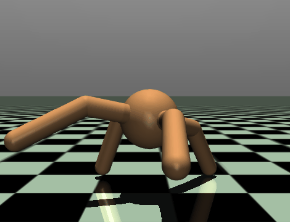
\includegraphics[width=0.45\linewidth]{figures/gym_ant_mujoco.png}%
		\label{fig:ant}%
	}%
	\caption{In figure \ref{fig:landing} (left) the goal is to land securely the spaceship (in pruple). In figure \ref{fig:translation_attn} (right) the goal is for the ant to balance itself and start walking.}
	\label{fig:faramas-gym}
\end{figure}

\subsection{Environment dynamics}
\label{sec:env_dyn}

The way that Farama's gym models agent-environment interaction is quite similar to what we explained in section \ref{sec:form-intro-rl}. In the listing \ref{code:init_env} we see a basic example of how an interaction with an environment can be performed. First, we need to instantiate the environment, calling the \inlinecode{gym.make} function, with the argument passed as the name of the environment we are going to interact. In order to initialize the environment, we must reset it, using the \inlinecode{env.reset()} method. Once we have our environment ready, we can proceed to interact with it performing actions. The number of actions, called action space, varies depending on the environment, but the gymnasium library offers methods and attributes that facilitate them in run-time, such as \inlinecode{env.action_space.n}. In the example provided, the action taken is random, using \inlinecode{env.action_space.sample()}, but we can use more complex methods to select the action our agent is going to perform (i.e. a neural network). 

\begin{lstlisting}[caption={Initialization of an environment in Farama's gymnasium}, label={code:init_env}]
import gymnasium as gym
env = gym.make("LunarLander-v2", render_mode="human")
observation, info = env.reset(seed=42)
for _ in range(1000):
	action = env.action_space.sample() 
	observation, reward, terminated, truncated, info = env.step(action)
	
	if terminated or truncated:
	observation, info = env.reset()

env.close()
\end{lstlisting}

In the RL framework, when an action is selected, the agent performs said action in the environment, and obtains a reward and a next observation. In the code, method \inlinecode{env.step()} is in charge of doing so, simulating what the outcome will be, returning the following:

\begin{itemize}
	\item \textbf{Observation}: What the environment lets the agent see about its state. If $\text{state}=\text{observation}$ then the environment is a MDP, if not, then its a POMDP.
	\item  \textbf{Reward}: The numerical signal that represents how good (or bad) the actions the agent is taking are.
	\item \textbf{Terminated}: Boolean flag that represents if the episode has ended.
	\item  \textbf{Truncated}: Boolean flag that represents if there has been an unexpected situation that resulted in the current episode ending prematurely. 
	\item \textbf{Info}: Additional information from the current state of the environment, such as current lives if the game is a survival, the current score or even and additional final observation if the state is terminal.
\end{itemize}

The interacting loop could go forever if no additional condition is stated, that is why using the truncated and terminated flags is the common approach to reset the environment and start a new episode. Once the simulation is over, we can close the environment using the \inlinecode{env.close()} method.

\subsection{Processing techniques of an environment}
\label{sec:proc_env}

In most of the environments, observations are usually RGB frames displaying the current situation of the environment. Since our models deal with visual data, it is quite convenient to use some pre-processing techniques that simplify the observation into something that is more "consumable" by the DQN agent. Farama's gymnasium provides an API that allows modifications of the environment, called \textbf{wrappers}. These wrappers are conceived so that they can alter the original behaviour of the environment, in terms of the reward, number of frames skipped between steps or the colour gamut of the observation. 

In our implementation, we make use of four custom wrappers, along with some pre-defined offered by the gymnasium library. This will ease the observation processing a make lightweight computations by discarding redundant information provided by the environment. In the following section we explain some of the custom wrappers that we have developed, along with some pre-defined ones.

\subsubsection{Skip N-Frames}
\label{sec:skip_wrapper}
In a RL environment, the variation between two consecutive frames usually is very little. If we pass each observation the environment provides, we end up with lots of redundant information which means that lots of computational resources are used in vane. One of the main approaches that is done in RL and other fields such as robotics or autonomous driving, where high frequency sensors are used is to skip a fixed amount of frames per observation. This technique is usually known as "frame skipping". The code developed for this wrapper is shown in listing \ref{code:skip_wrapper}. One thing to note is that in terms of reward, we add in the n-th frame the accumulated rewards from the skipped observations, since we are comprising the information of n-frames in just one observation.

\begin{lstlisting}[caption={Frame skip wrapper}, label={code:skip_wrapper}]
class SkipFrame(gym.Wrapper):
	def __init__(self, env: gym.Env, skip):
	"""Returns only the `skip`-th frame."""
		super().__init__(env)
		self._skip = skip
	
	def step(self, action):
	"""Repeat action, and sum reward"""
		total_reward = 0.0
		for _ in range(self._skip):
			obs, reward, done, trunk, info = self.env.step(action)
			total_reward += reward
			if done or trunk:
				break
	
	return obs, total_reward, done, trunk, info

\end{lstlisting}

\subsubsection{Gray-Scale Observation}
Most of the gymnasium's environments are in RGB colour coding. This may be useful for us humans, since we can extract additional information about the state of the game (i.e. detect if the ghosts in the Pac-man game are or colour blue or not, which gives us a hint on wether we can "eat" them and win points). Machine vision does not work like this, and this information sometimes is seen as redundant, since for a machine, the greyscale palette is enough. Also, it has its limitations in terms of computing power and resources. RGB images have three channels, which makes the observations more expensive to process, specially if we are stacking n-frames to them. Also, since we are dealing with experience replay models, storing these observations along with the collected experience can result in more memory consumption, which is not optimal in the training process. To solve this, the RGB observations are transformed to integer grey-scale. In this case, we are going to make use of PyTorch's transforms from the torchvision library that adds several visual transformations such as cropping, rotation, inversions or colour palette transformations. Using these transformations, we can also cast the original data-type of the observation (\inlinecode{numpy.array}) to a \inlinecode{torch.Tensor} datatype, which is convenient for processing said observation using a neural network using PyTorch framework. The code developed to apply this transformation to the environment is displayed in listing \ref{code:grayscale_wrapper}.

\begin{lstlisting}[caption={Grayscale frame wrapper}, label={code:grayscale_wrapper}]
class GrayScaleObservation(gym.ObservationWrapper):
	def __init__(self, env: gym.Env):
		super().__init__(env)
		obs_shape = self.observation_space.shape[:2]
		# since we are wrapping the observation that an environment provides,
		# we must update the observation space to match the new wrapped env.
		self.observation_space = Box(low=0, high=255, shape=obs_shape, dtype=np.uint8)
	
	def permute_orientation(self, observation):
		# permute [H, W, C] array to [C, H, W] tensor for pytorch model
		observation = np.transpose(observation, (2, 0, 1))
		observation = torch.tensor(observation.copy(), dtype=torch.float)
		return observation
	
	def observation(self, observation):
		observation = self.permute_orientation(observation)
		# since we have updated the observation space attribute, we must 
		# do so with the pixels from the env, casting them from RGB to grayscale
		transform = T.Grayscale()
		observation = transform(observation)
		return observation
	
\end{lstlisting}

\subsubsection{Resize Observation}
The size of an image is a crucial element in neural networks for visual data processing, a larger image is preferable, but it also comes at a cost, specially in the training stage. High resolution images require deeper and bigger models to capture all the spatial features, which results in more parameters to adjust during training. The issue comes with the availability of computational resources, since we do not have a cluster with multiple GPUs at our disposal. To adapt to our computational resources, we have added an additional custom wrapper to our environment that resizes the observation from its original shape, $256 \times 240$ to a down-scaled shape of $84 \times 84$. The code for doing so is portrayed in listing \ref{code:resize_wrapper}, where we use torchvision's transforms for doing so. Additionally, we normalize the pixel values by using the \inlinecode{T.Normalize(0,255)} transform.

\begin{lstlisting}[caption={Resize frame wrapper}, label={code:resize_wrapper}]
class ResizeObservation(gym.ObservationWrapper):
	def __init__(self, env: gym.Env, shape):
		super().__init__(env)
		# If shape is just a number it creates a tuple with that same number (i.e. 84 -> (84,84))
		# if is a list creates a "tuple" object with the given shape
		if isinstance(shape, int):
		self.shape = (shape, shape)
		else:
		self.shape = tuple(shape)
		
		obs_shape = self.shape # + self.observation_space.shape[:2]
		self.observation_space = Box(low=0, high=255, shape=obs_shape, dtype=np.uint8)
	
	def observation(self, observation):
		# Use torch transforms to resize the observation 
		# to the wanted resize resolution
		transforms = T.Compose(
			[T.Resize(self.shape, antialias=True),
			T.Normalize(0,255)]
		)
		
	# apply the transformation
	observation = transforms(observation).squeeze(0)
	return observation
	
\end{lstlisting}

\subsubsection{Additional Wrappers}
Additionally, there are some libraries such as Stable Baselines 3 \cite{stable-baselines3} or TorchRL \cite{bou2023torchrl} that provide methods and classes that encapsulate lots of the functionality provided by wrappers which were useful for our experiments:

\begin{itemize}
	\item \textbf{ClipRewardEnv}: Maps the original reward signal from the environment to the range [-1, 1]. This has multiple benefits, such as preventing larger gradients that may affect learning due to outliers in the reward distribution or encourage exploration, since the algorithm will not always go for high-reward actions, since all of them are within a small range. This is further explored in works such as \cite{Eschmann2021} where they remark the importance of designing an optimal reward signal for the agent to boost its behaviour.
	\item \textbf{EpisodicLifeEnv}: For games where the agent has several lives, treats losing a life as the end of the episode. This was originally implemented by Silver \textit{et al.} in \cite{mnih2013playing} to help the agent with value estimation.
	\item \textbf{MaxAndSkipEnv}: Frame skipping with some truncated behaviour (similar to what we have already explained in section \ref{sec:skip_wrapper}).
	\item \textbf{NoopResetEnv}: Once the environment is reset, during a certain amount of steps, the agent performs no actions (\textbf{no-op}erations) over the environment.
\end{itemize}

 While it may be true that RL is not the field in AI that receives the most attention, little by little, lots of frameworks and libraries that make quite easy train a model are being launched. Both TorchRL and Stable Baselines are quite useful libraries, and since they are PyTorch oriented, they helped us quite a lot in the development of this work.

\section{Agents development}
\label{sec:agents_dev}

\subsection{DQN  and DDQN training loop}
\label{sec:dqn_training_loop}
\subsubsection{Explaining the algorithm}
Once we had our environment ready for the agent to play, we proceeded to develop the DQN algorithm as Silver \textit{et al.} defined in \cite{mnih2013playing}. In this section we will first explain the algorithm and the we will briefly explain how we program it using pure python and PyTorch.

\begin{algorithm}
	\caption{DQN with Experience Replay}
	\label{alg:dqn}
	\begin{algorithmic}[1]
		\State Initialize replay memory $D$ to capacity $N$
		\State Initialize action-value function $Q$ with random weights
		\State Initialize target action-value function $\hat{Q}$ with weights $\theta^{-} = \theta$
		\For{episode = 1, $M$}
		\State Initialize sequence $s_1 = \{x_1\}$ and pre-processed sequence $\phi_1 = \phi(s_1)$
		\For{t = 1, $T$}
		\State With probability $\epsilon$ select a random action $a_t$
		\State otherwise select $a_t = \arg\max_a Q(\phi(s_t), a; \theta)$
		\State Execute action $a_t$ in emulator and observe reward $r_t$ and image $x_{t+1}$
		\State Set $s_{t+1} = s_t, a_t, x_{t+1}$ and preprocess $\phi_{t+1} = \phi(s_{t+1})$
		\State Store transition $(\phi_t, a_t, r_t, \phi_{t+1})$ in $D$
		\State Sample random mini-batch of transitions $(\phi_j, a_j, r_j, \phi_{j+1}) \sim D$
		\State Set $y_j = 
		\begin{cases} 
			r_j & \text{if episode terminates at step } j+1 \\
			r_j + \gamma \max_{a'} \hat{Q}(\phi_{j+1}, a'; \theta^{-}) & \text{otherwise}
		\end{cases}$
		\State Perform a gradient descent step on $(y_j - Q(\phi_j, a_j; \theta))^2$ with respect to the network parameters $\theta$
		\State Every $C$ steps reset $\hat{Q} = Q$
		\EndFor
		\EndFor
	\end{algorithmic}
	
\end{algorithm}

The algorithm is defined in \ref{alg:dqn}, where first we define a replay memory. This replay memory is basically a data structure that focus on storing experiences that the agent performs in the environment. Formally, we define as experience the tuple as $(\phi_t, a_t, r_t, \phi_{t+1})$, although when developing the code, we made some minor adjustments for better performance and extended functionality, such as store if the experience resulted in a terminal state. Also, we initialize our action-value function approximator $Q$ with random weights, which we will call the online approximator. From there, we will create our target network (the look-ahead), that will be defined as $\hat{Q}$ and copy the weights $\theta$ from $Q$ (the online/estimation network) to $\hat{Q}$. This ensures that the online function approximator and the target function approximator start the training process under equal circumstances, avoiding inaccurate estimation for the state-action values.

Once these initialization steps are done, we begin the training loop, where we iterate for a fixed number of episodes $N$ in the training process. Since we want to extract the most relevant features, we assume that there is a function $\phi$ that will pre-process the environment, extracting the most relevant features from our input $x_t$ creating the feature vector $s_t$. For us, this would be the wrappers explained in section \ref{sec:proc_env}. Then, the episode begin and, for each time step t, up until the episode ends (the agent finds itself in a terminal state) the agent starts playing and learning.

Both DQN and DDQN follow an $\epsilon$-greedy policy as the behavioural policy $\pi$, meaning that with a probability $\epsilon$ a random action will be selected instead of the one most rewarding one, according to our $Q$-value estimation. This encourage exploration, and not falling into a sub-optimal set of $Q$-values as explained in \cite{exploitation_vs_exploration}, where the exploration vs. exploitation dilemma is discussed. For our implementation, we will have and initial exploration rate $\epsilon_0$ and a final exploration rate $\epsilon_f$ and we designed a scheduling that decays the value of $\epsilon$. Doing so provides an exploration stage at first, where the agent is forced to perform lots of random actions, experimenting and evaluating different situations, thus, increasing the variability of the states that it can learn from.

Once the action is performed, the environment will react to it, providing a reward for such action and a new raw observation $x_{t+1}$. This will create a transition tuple that will be stored in the replay memory buffer $D$. 

As DQN is an off-policy algorithm, we will learn by performing actions that do not follow the behavioural policy $\pi$ but the target policy $\mu$. By doing so, we will sample a transition tuple from the replay memory $D$, and applying the greedy policy obtaining the $Q$-values obtained as the target $y_j$ for the $s_{t+1}$ (the look-ahead) of the sampled transition tuple. For the online network, we will compute the $Q$-values for the current state $s_t$ and apply action selection using the greedy policy, obtaining the agent estimations for the current state. As explained in section \ref{sec:val-fun_approx}, by minimizing this loss as the TD-error, we are teaching the online network to base the value estimations of the current state $s_t$ using the target network estimations $s_{t+1}$. This could be seen as a "look-ahead" view that glances into the "future" to obtain more information about how good the current state is. Once we got loss value, we adjust the online network weights $\theta$ to minimize the loss using the gradient descent algorithm. 

Finally, when a fixed number of steps has passed, we will copy the online network parameters $\theta$ onto the target network, so that the distribution of the parameters from the target network do not diverge too much from the online network.

\subsubsection{Main loop implementation}
While the DQN algorithm seems quite straight forward on paper, the implementation tells other story. For doing so, we implemented several modules to compartmentalize the different functionalities. By making the code modular, the process of improving the code, add new functionalities and connect different modules was easier, creating a pipeline that allowed to test several training set-ups in parallel.

The main script is called \href{https://github.com/Javimh18/DL_TFM/blob/main/src/train.py}{train.py} which basically loads all the hyper-parameters that the code needs, such as $\gamma$ for the target estimation or the learning rate when adjusting the net hyper-parameters given the loss. After that, it initializes the agent, that can be of two types, DQN or DDQN to then pass all these arguments into the \href{https://github.com/Javimh18/DL_TFM/blob/main/src/trainer.py}{Trainer} class. This class implements the main functionality explained in algorithm \ref{alg:dqn}, and a code snippet is presented in listing \ref{code:trainer_main_loop}. We will go deeper into this class in the following sections, but for now we will only explain the main functionality. First, we reset the environment, and using the done and truncated flags provided by the agent, we can check whether the episode finishes or not. Then, the agent performs an action according to the action-state values over the environment, obtaining a transition tuple which is stored in the replay memory. Finally, the agent learns from the pool of experiences stored in the replay buffer.

\begin{lstlisting}[caption={Trainer main loop}, label={code:trainer_main_loop}]
while self.curr_step < self.n_steps:
	# reset environment
	done, trunc = False, False
	state = self.env.reset()
	#measure_array = []
	while (not done) and (not trunc):
		# 1. get action for state
		action = self.agent.perform_action(state, self.curr_step)  
		# 2. run action in environment
		next_state, reward, done, trunc, info = self.env.step(action) 
		# 3. collect experience in exp. replay buffer for Q-learning
		self.agent.store_transition(state, action, reward, next_state, done, trunc) 
		# 4. Learn from collected experiences
		q, loss = self.agent.learn(self.curr_step)
		# 5. Update the current state 
		state = next_state
		# 6. Update step value 
		self.curr_step += 1            
		logger.log_step(loss, q)

	if 'episode' in info:
		# episode field is stored in the info dict if episode ended
		logger.log_episode(ep_length=info['episode']['l'], ep_reward=info['episode']['r'],)
		if not(self.curr_episode % self.log_every) :
			logger.record(episode=self.curr_episode, 
									epsilon=self.agent.exploration_rate, 
									step=self.curr_step)
			# log the real reward using episode statistics
		self.curr_episode += 1
	
\end{lstlisting}

\subsubsection{Digging deeper: the DQN agent}
\label{sec:digging_dqn_agent}

Once we have seen the training loop, we are going to delve into the agent functionality (\href{https://github.com/Javimh18/DL_TFM/blob/main/src/agents/dqn_agent.py}{dqn\_agent.py}). 

\begin{lstlisting}[caption={Perform action method from the DQN Agent}, label={code:ex_action}]
@torch.no_grad()
def perform_action(self, state, t):
	# decide wether to exploit or explore
	if np.random.random() < self.exploration_rate:
		action =  np.random.randint(0, self.action_dim)
	else:
		# use of __array__(): https://gymnasium.farama.org/main/_modules/gymnasium/wrappers/frame_stack/
		state = first_if_tuple(state).__array__()
		state = torch.tensor(state, device=self.device).unsqueeze(0)
		q_values = self.net(state, model='online')
		action = torch.argmax(q_values, dim=1).item()
	
	# decrease exploration_rate according to scheduler
	self.exploration_rate = self.exp_scheduler.step(t)
	self.exploration_rate = max(self.exploration_rate_min, self.exploration_rate)
	
	return action
\end{lstlisting}

As we have seen in the listing \ref{code:trainer_main_loop}, the first thing that our agent does is execute an action. According to algorithm \ref{alg:dqn}, we perform the action according to the target policy. We can see the code in the listing \ref{code:ex_action} the \inlinecode{perform\_action} method when we pick the action that maximizes the action values. After that, we update the exploration scheduler. The exploration scheduler updates the exploration rate $\epsilon$ for each time-step with the \inlinecode{step}. We have used three different types of functions to do so: exponential, linear and product of exponentials, which we will talk about in following sections. After the agent selects the action, we store the transition in the replay memory module of the agent using the \inlinecode{store\_transition}. In our case, we opted to use \inlinecode{TensorDictReplayBuffer} module from TorchRL, since it has seamless integration with PyTorch, making it quite easy to use and efficient to run, as we can store the replay memory in the GPU, avoiding for bottlenecks in the training process runtime. Inside, this implementation of the replay buffer stores an array of transition tuples as tensors. When the agent samples from the replay memory, it can be done using mini-batches, making the training process more efficient. In the listing \ref{code:replay_memory_dqn} we define the replay memory buffer, where we can state the size of the memory in terms of transition tuples, the device where the replay memory is stored, the sampler or if the replay memory has a mapping to disk in case we have limited storage resources. Additionally, we can also define the algorithm to follow in the sampling process. In our case, we opted to use prioritized experience replay sampling \cite{schaul2016prioritized} which basically prioritizes more significant experiences based on higher temporal-difference errors during training, enhancing learning. The motivation behind this work is similar to what happens in unbalanced datasets, as the less frequent classes usually are the hardest to recognize for the classifier. In order to mitigate this, different techniques ensure to weight more importance sampling to the less frequent instances in the dataset. 

\begin{lstlisting}[caption={Code snippet for the replay memory of the DQN agent}, label={code:replay_memory_dqn}]
# defining the memory (experience replay) of the agent
self.memory = TensorDictReplayBuffer(storage=LazyMemmapStorage(
	max_size=float(agent_config['replay_memory_size']),
	scratch_dir='./memmap_dir',
	device=self.device,
	),sampler=PrioritizedSampler(max_capacity=int(float(agent_config['replay_memory_size'])), 
	alpha=1.0, 
	beta=1.0)
)
\end{lstlisting}

Storing different experiences along the exploration stage tries to ensure that by the time the agent starts to learn by back-propagation, there is enough data variability to capture enough different situations in the environment to learn to act in most of them. In our implementation, the learning process is done by the \inlinecode{learn} method from the agent class. We present the function in listing \ref{code:learn_dqn_fun}, where first, we have a series of if statements that check several conditions. The first if statement checks that a fixed number of steps has passed in the training to synchronize the online and target network parameters (i.e. $\theta_{online} \rightarrow \theta_{target}$). After that, we check if a fixed number of training steps has passed to save the state of the network periodically. In order to fill the replay memory buffer before start to learn from it, we define a number of steps where the network does nothing, called burning, that ensures that, by the time the network starts to adjust its weights, there is enough variability of experiences to learn from. Also, for computational resources purposes, we made the network learn only every \inlinecode{learn_every} steps.

\begin{lstlisting}[caption={\inlinecode{learn} function from the DQN agent}, label={code:learn_dqn_fun}]
def learn(self, step):
	
	# Once the error is computed, each sync_every the weights of the 
	# target network are updated to the online network
	if not (step % self.sync_every):
		self.sync_Q_target()
	
	# save the model each save_every steps
	if not (step % self.save_every) and step > 0:
		self.save(step)
	
	# Burning lets episodes pass but collects experiences for the memory buffer
	if step < self.burning:
		return None, None
	
	# Not learning every step, but every "learn_every" steps
	if step % self.learn_every != 0:
		return None, None
	
	state, action, reward, next_state, done, _ = self.recall()
	
	# once we have our transition tuple, we apply TD learning over our DQN and compute the loss
	q_estimate = self.compute_q_estimate(state, action)
	q_target = self.compute_q_target(reward, done, next_state)
	
	# update the q_online network using the loss
	loss = self.loss_fn(q_target, q_estimate) # Compute Huber loss
	self.optimizer.zero_grad()
	loss.backward()
	self.optimizer.step()
	
	return q_estimate.mean().item(), loss.item()
\end{lstlisting} 

After these checks, we start with the learning process. To do so, we first recall or sample from the replay buffer with a defined sample size (i.e. 8, 16, 32... etc.) that extract a set of samples for the model to learn. Thanks to tensor operation support provided from PyTorch, this is forwarded through the online and target networks seamlessly. The \inlinecode{compute\_q\_target} method implements the TD target element in the DQN loss equation \ref{eq:dqn_loss} which is $r + \gamma \max_{a'} Q(s', a'; w^-))$, while the method \inlinecode{compute\_q\_estimate} implements the TD estimate which is $Q(s, a; w)$ where actions $a$ and $a'$ are selected according to the target greedy policy for the sampled state s from the buffer and its corresponding next state s'.

With the TD values, we compute the loss. We opted for the Huber Loss \cite{9918637}, defined in equation \ref{eq:hub_loss} where $\delta$ is a regularization parameter. This type of loss is useful in these set-ups, thanks to its robustness to outliers in the data compared to the mean squared error loss function, which is of convenience for this problem in cases where loss between Q values estimates fall far over the hyper-parameter $\delta$.

\begin{equation}
	\label{eq:hub_loss}
	L_{\delta}(y, f(x)) = 
	\begin{cases} 
		\frac{1}{2}(y-f(x))^2 & \text{for $|y-f(x)| \leq \delta$, } \\
		\delta \cdot \left(|y-f(x)| - \frac{1}{2}\delta \right) & \text{otherwise}
	\end{cases}
\end{equation}

Finally, once the loss is computed, we perform the back-propagation process in the online network to adjust its weights and we return the mean Q-values for the sampled mini-batch.

\subsubsection{DDQN training loop: A minor update}
\label{sec:ddqn_training_loop}
In \cite{vanhasselt2015deep}, Van Hasselt \text{et al.} proposed an updated version of the DQN algorithm. As explained in section \ref{sec:val-fun_approx}, the overestimation bias from the DQN comes from the target evaluating and selecting the actions from the target network. To mitigate this, they propose to decouple the action selection for the TD-target, using the online network and evaluating that action with the target network. We apply the same changes for the DDQN agent as can be seen in listings \ref{code:dqn_action_selection} and \ref{code:ddqn_action_selection}. Since the functionality of the DDQN agent is exactly the same as the DQN, except for the TD target value, we made the DDQN agent class inherit from the DQN agent in the \href{https://github.com/Javimh18/DL_TFM/blob/main/src/agents/ddqn_agent.py}{ddqn\_agent.py} script, taking advantage of the already developed code.

\begin{lstlisting}[caption={DQN action selection algorithm}, label={code:dqn_action_selection}]
@torch.no_grad() # since this is our "ground truth" (look ahead prediction)
def compute_q_target(self, reward, done, next_state):
	q_next_max_value, _ = torch.max(self.net(next_state, model='target'), dim=1)
	return reward + (1 - done.float()) * self.gamma * q_next_max_value
\end{lstlisting}

\begin{lstlisting}[caption={DDQN action selection algorithm}, label={code:ddqn_action_selection}]
@torch.no_grad() # since this is our "ground truth" (look ahead prediction)
def compute_q_target(self, reward, next_state, done):
	# for the next state, get the actions that have higher q_values
	online_q_action_value = self.net(next_state, model='online')
	max_value_action = torch.argmax(online_q_action_value, dim=1)
	# then, apply those actions onto the target (off-line) model
	target_q_action_values = self.net(next_state, model='target')
	q_next_max_value = target_q_action_values[np.arange(0, self.batch_size), max_value_action]
	
	return (reward + (1-done.float()) * self.gamma * q_next_max_value).float()
\end{lstlisting}

\subsection{Attention-based models: Vision Transformer}
\label{sec:vit_transformer_imp}
The aim of this work is to test out if there is any explain-ability in the decision making that agents perform when the value function is an approximator, which is an ideal set-up for DQN learning. For this section we will discuss the implementation of the attention-based models (i.e. vision transformers) that were used to carry out our experiments. First, we will talk about the Vision Transformer, discussing about the relevant aspects involved from the intuition to the actual implementation, that we took from \cite{caron2021emerging}. 

In several implementations for the vision transformer, we see that one of the most important things is for the model to be flexible to different configurations, where the number of blocks, embedding dimension or the number of heads in the multi-head attention block changes. This leads to easier ways to try out different configurations for the training process. For this section, first we are going to go over the constructor of the model and discuss its several parts. After that we will delve in the implementation of the most relevant.

\subsubsection{Constructor}
The constructor of the ViT is portrayed in listing \ref{code:vit_constructor}. We can see that the class is flexible to parametrizations, since we can specify the image size, the patch size, the channel of the input or the embedding dimension. In general terms, the constructor initializes the patch embedding module. This component is in charge of taking the input image and extract the patches from the spatial coordinates while enlarging the channel dimension from in channels to the embedding dimension. After that, it declares two essential parameters for the ViT: the class token and the positional embedding, which both of them are self learnable parameters that the network adjust during training. The next main component is a sequence of ViT blocks, which are implementations of the transformer encoder which are stacked one on top of each other. Finally, we have the classification head, which maps from the embedding dimension of the class token vector to the output dimension of the network, producing the corresponding Q value of an action as an output. We would also like to notice that for this implementation to work with the DDQN algorithm, we made some minor adaptations to the code, such as adding some additional dense layers to map from the feature space to the action space.

\begin{lstlisting} [caption={ViT model initialization}, label={code:vit_constructor}]
def __init__(self, img_size=224, patch_size=16, in_chans=3, num_classes=0, embed_dim=768, depth=12,
	num_heads=12, mlp_ratio=4., qkv_bias=False, qk_scale=None, drop_rate=0., attn_drop_rate=0.,
	drop_path_rate=0., norm_layer=nn.LayerNorm, **kwargs):
	super().__init__()
	self.num_features = self.embed_dim = embed_dim
	
	self.patch_embed = PatchEmbed(
	img_size=img_size, patch_size=patch_size, in_chans=in_chans, embed_dim=embed_dim)
	num_patches = self.patch_embed.num_patches
	
	self.cls_token = nn.Parameter(torch.zeros(1, 1, embed_dim))
	self.pos_embed = nn.Parameter(torch.zeros(1, num_patches + 1, embed_dim))
	self.pos_drop = nn.Dropout(p=drop_rate)
	
	dpr = [x.item() for x in torch.linspace(0, drop_path_rate, depth)]  # stochastic depth decay rule
	self.blocks = nn.ModuleList([
		Block(
		dim=embed_dim, num_heads=num_heads, mlp_ratio=mlp_ratio, qkv_bias=qkv_bias, qk_scale=qk_scale,
		drop=drop_rate, attn_drop=attn_drop_rate, drop_path=dpr[i], norm_layer=norm_layer)
		for i in range(depth)])
	self.norm = norm_layer(embed_dim)
	
	# Classifier head
	self.head = nn.Linear(embed_dim, num_classes) if num_classes > 0 else nn.Identity()
	
	trunc_normal_(self.pos_embed, std=.02)
	trunc_normal_(self.cls_token, std=.02)
	self.apply(self._init_weights)
\end{lstlisting}

\subsubsection{Patch Embedding}
The patch embedding module is of great importance, since it is what transforms the visual data into something that is "consumable" for the ViT. The code of the patch embedding is in listing \ref{code:patch_embedding}. To perform the patch projections, they use a trick leveraging the 2D convolutional operator, where they specify the filter size and the stride as the size of the patch. This ensures that the projections are non-overlapping and reduced in the spatial dimension. Additionally, since we want the channels to be projected from the \inlinecode{in\_channels} dimension to the embedding dimension, the number of filters specified in the 2D convolution operator is the same as the embedding dimension. With this trick, the implementation is more efficient and readable, providing the embedded patches from the original image.

\begin{lstlisting}[caption={Patch Embedding module}, label={code:patch_embedding}]
class PatchEmbed(nn.Module):
	""" 
	Image to Patch Embedding
	"""
	def __init__(self, img_size=224, patch_size=16, in_chans=3, embed_dim=768):
	super().__init__()
	num_patches = (img_size // patch_size) * (img_size // patch_size)
	self.img_size = img_size
	self.patch_size = patch_size
	self.num_patches = num_patches
	
	self.proj = nn.Conv2d(in_chans, embed_dim, kernel_size=patch_size, stride=patch_size)
	
	def forward(self, x):
		B, C, H, W = x.shape
		x = self.proj(x).flatten(2).transpose(1, 2)
		return x
\end{lstlisting}

\subsubsection{ViT encoder block}
Once we have our embedded image, we can proceed to process it using the ViT encoder blocks. The code of a single block is depicted in listing \ref{code:vit_block_implementation}. The input of a single block is either the embedded input image of the previous block output, to which the self attention layer will be applied, or the original image embedded. We will delve into the implementation of the attention layer after, but for now, the only thing we ought to know is that the attention layer returns the input embedding pondered by the importance of each patch. After that, it applies an projection to a layer with four times the embedding dimension to then apply a dropout layer. Since these models are very deep, in the forward pass we see that a residual connection \cite{he2015deep} is implemented, that eases the gradient flow in the back-propagation stage.

\begin{lstlisting}[caption={ViT blocks implementation}, label={code:vit_block_implementation}]
class Block(nn.Module):
	def __init__(self, dim, num_heads, mlp_ratio=4., qkv_bias=False, qk_scale=None, drop=0., attn_drop=0.,
		drop_path=0., act_layer=nn.GELU, norm_layer=nn.LayerNorm):
		super().__init__()
		self.norm1 = norm_layer(dim)
		self.attn = Attention(
		dim, num_heads=num_heads, qkv_bias=qkv_bias, qk_scale=qk_scale, attn_drop=attn_drop, proj_drop=drop)
		self.drop_path = DropPath(drop_path) if drop_path > 0. else nn.Identity()
		self.norm2 = norm_layer(dim)
		mlp_hidden_dim = int(dim * mlp_ratio)
		self.mlp = Mlp(in_features=dim, hidden_features=mlp_hidden_dim, act_layer=act_layer, drop=drop)
	
	def forward(self, x, return_attention=False):
		y, attn = self.attn(self.norm1(x))
		if return_attention:
			return attn
		x = x + self.drop_path(y)
		x = x + self.drop_path(self.mlp(self.norm2(x)))
	return x
\end{lstlisting}

\subsubsection{ViT Attention Module}
The attention blocks are the core functionality of this model. The code from the implementation is in listing \ref{code:attn_block}. In the constructor of the module, we can see that to compute the dimension of each head, it divides the embedding dimension by the number of heads we are going to apply. After that, it defines the weight matrices of the query, key and value from the self-attention module. To do so, it uses another trick to reduce the number of the layer's weights, by multiplying by three the embedding dimension, and then rearranging the tensor, so the highest order dimension is the one which contains the query, key and value values of the attention layer. After that it performs the self-attention operation, according to the equation \ref{eq:attn_eq}, obtaining the pondered embeddings. Finally, it performs some additional linear projections to obtain the final embedding. One thing that is of great use from this ViT block is that, it also returns the attentions maps from the attention blocks.

\begin{lstlisting}[caption={Attention module for the ViT model}, label={code:attn_block}]
class Attention(nn.Module):
	def __init__(self, dim, num_heads=8, qkv_bias=False, qk_scale=None, attn_drop=0., proj_drop=0.):
		super().__init__()
		self.num_heads = num_heads
		head_dim = dim // num_heads
		self.scale = qk_scale or head_dim ** -0.5
		
		self.qkv = nn.Linear(dim, dim * 3, bias=qkv_bias)
		self.attn_drop = nn.Dropout(attn_drop)
		self.proj = nn.Linear(dim, dim)
		self.proj_drop = nn.Dropout(proj_drop)
	
	def forward(self, x):
		B, N, C = x.shape
		qkv = self.qkv(x).reshape(B, N, 3, self.num_heads, C // self.num_heads).permute(2, 0, 3, 1, 4)
		q, k, v = qkv[0], qkv[1], qkv[2]
		
		attn = (q @ k.transpose(-2, -1)) * self.scale
		attn = attn.softmax(dim=-1)
		attn = self.attn_drop(attn)
		
		x = (attn @ v).transpose(1, 2).reshape(B, N, C)
		x = self.proj(x)
		x = self.proj_drop(x)
		return x, attn
\end{lstlisting}

\subsubsection{The forward method}
With these main modules from the ViT explained, we can now address the \inlinecode{forward} method from the ViT class, which is portrayed in listing \ref{code:vit_forward}. First, the \inlinecode{forward} method calls \inlinecode{prepare_tokens}, which is a function that encapsulates the patch embedding functionality plus the initialization of the positional encoding and the concatenation of the token class to the patch embedding tensor, as shown in figure \ref{fig:attn_maps}. After that, the positional embedding is added to the embedded tensor, giving additional context on how the patches are arranged, to then be passed to the ViT blocks. The ViT blocks are held into a \inlinecode{ModuleList} type of object from PyTorch's library. This enables creating lists where each element is a \inlinecode{nn.Module}, which can be tracked down by PyTorch's graph engine to perform forward and backward passes. The code iterates over the list of blocks, to then obtain a normalized embedding using a \inlinecode{NormLayer} module. Finally, to project from the embedding class to the action space, we perform a linear projection and obtain the class token indexing by \inlinecode{x[:, 0]}.

\begin{lstlisting}[caption={ViT forward method}, label={code:vit_forward}]
def prepare_tokens(self, x):
	B, nc, w, h = x.shape
	x = self.patch_embed(x)  # patch linear embedding
	
	# add the [CLS] token to the embed patch tokens
	cls_tokens = self.cls_token.expand(B, -1, -1)
	x = torch.cat((cls_tokens, x), dim=1)
	
	# add positional encoding to each token
	x = x + self.interpolate_pos_encoding(x, w, h)
	
	return self.pos_drop(x)
	
def forward(self, x):
	x = self.prepare_tokens(x)
	for blk in self.blocks:
		x = blk(x)
	x = self.norm(x)
	x = self.head(x)
	return x[:, 0]
\end{lstlisting}

If the reader wants to see the code in depth, this implementation is in the \href{https://github.com/Javimh18/DL_TFM/blob/main/src/models/vit.py}{vit.py} script, under the models folder from the repository.

\subsection{Attention-based models: SWIN Transformer}
\label{sec:swin_transformer_rl}
In this section we will do something similar to section \ref{sec:vit_transformer_imp}, where first we will talk about the intuition the changes with respect to the vision transformer, and then we will go over the implementation of those changes, using the code from \cite{liu2021swin}, since this model is actually more complex in the development aspect that the ViT. Another thing to note is that we will not go over the whole code used and implemented for these models, instead, we will give a comprehensive review of the implementation and delve only into the most critical aspects of them.

The SWIN transformer emerged as a version of the ViT that takes into account hierarchical features, resembling the convolutional neural networks approach to solve vision problems. It is composed from different stages, that hold different blocks. Additionally, the model introduces spatial dimension reduction, which is a big change in terms of how the model interact and manipulates the data. Additionally, it introduces the concepts of windows in order to reduce the computational overhead of the self-attention operation. In listing \ref{code:swin_transformer_constructor} we a reduced version of the original implementation. 

\subsubsection{Constructor}
One of the main changes that the SWIN Transformer introduces is the positional embedding, which is relative between patches, instead of absolute as the ViT. The main reason behind this is the fact that the patches are now within windows, and the attention is computed within those windows, so each patch should have some kind of notion on where the other patches inside its window are. Additionally, the declaration of the SWIN layers follows exactly the same logic as the ViT, but with a minimal difference. According to figure \ref{fig:swinarchitecture} from section \ref{sec:swin-transformer} we want for each SWIN stage to have different SWIN transformer layers, and, at the end, a patch merging transformation to reduce the spatial dimension. To do so, the BasicLayer module contains a flexible set-up where parameters such as number of heads, the depth for each layer or the window size may vary depending on the stage where is declared. The implementation is also flexible to a variable number of BasicLayer layers, since it uses the \inlinecode{ModuleList} object.

\begin{lstlisting} [caption={SWIN Transformer constructor}, label={code:swin_transformer_constructor}]
class SwinTransformer(nn.Module):
	
	def __init__(self, img_size=224, patch_size=4, in_chans=3, num_classes=1000, embed_dim=96, depths=[2, 2, 6, 2], num_heads=[3, 6, 12, 24], window_size=7, mlp_ratio=4., qkv_bias=True, qk_scale=None, drop_rate=0., attn_drop_rate=0., drop_path_rate=0.1,	norm_layer=nn.LayerNorm, ape=False, patch_norm=True, use_checkpoint=False, **kwargs):
		super().__init__()
		
		# ... Already explained variables in VIT transformer + Patch Embedding
		
		# absolute position embedding
		if self.ape:
			self.absolute_pos_embed = nn.Parameter(torch.zeros(1, num_patches, embed_dim))
			trunc_normal_(self.absolute_pos_embed, std=.02)
		
		# ... Already explained variables in VIT transformer
		
		# build layers
		self.layers = nn.ModuleList()
		for i_layer in range(self.num_layers):
			layer = BasicLayer(dim=int(embed_dim * 2 ** i_layer),
						input_resolution=(patches_resolution[0] // (2 ** i_layer),
						patches_resolution[1] // (2 ** i_layer)),
						depth=depths[i_layer],
						num_heads=num_heads[i_layer],
						window_size=window_size,
						mlp_ratio=self.mlp_ratio,
						qkv_bias=qkv_bias, qk_scale=qk_scale,
						drop=drop_rate, attn_drop=attn_drop_rate,
						drop_path=dpr[sum(depths[:i_layer]):sum(depths[:i_layer + 1])],
						norm_layer=norm_layer,
						downsample=PatchMerging if (i_layer < self.num_layers - 1) else None,
						use_checkpoint=use_checkpoint)
			self.layers.append(layer)
			
		# ... Already explained variables in VIT transformer
		
		self.apply(self._init_weights)
\end{lstlisting}

\subsubsection{BasicLayer}
The \inlinecode{BasicLayer} module has inside of it the functionality that goes inside of every stage of the SWIN transformer. To do so, the class attribute \inlinecode{self.blocks} is declared as a \inlinecode{ModuleList} where the \inlinecode{SwinTransformerBlock} instances are declared. Since at the end of some stages, the patch merging module is applied, the \inlinecode{down-sample} boolean flag indicates whether that stage performs down-sampling via patch merging or not. The forward method is pretty straight-forward, as the code first iterates through the  \inlinecode{SwinTransformerBlock} instances and then down-samples the spatial resolution of the returned embeddings if needed.

\begin{lstlisting}
class BasicLayer(nn.Module):

	def __init__(self, dim, input_resolution, depth, num_heads, window_size,
		mlp_ratio=4., qkv_bias=True, qk_scale=None, drop=0., attn_drop=0.,
		drop_path=0., norm_layer=nn.LayerNorm, downsample=None, use_checkpoint=False):
		
		super().__init__()
		self.dim = dim
		self.input_resolution = input_resolution
		self.depth = depth
		self.use_checkpoint = use_checkpoint
		
		# build blocks
		self.blocks = nn.ModuleList([
			SwinTransformerBlock(dim=dim, input_resolution=input_resolution,
				num_heads=num_heads, window_size=window_size,
				shift_size=0 if (i % 2 == 0) else window_size // 2,
				mlp_ratio=mlp_ratio,
				qkv_bias=qkv_bias, qk_scale=qk_scale,
				drop=drop, attn_drop=attn_drop,
				drop_path=drop_path[i] if isinstance(drop_path, list) else drop_path,
				norm_layer=norm_layer)
		for i in range(depth)])
		
		# patch merging layer
		if downsample is not None:
			self.downsample = downsample(input_resolution, dim=dim, norm_layer=norm_layer)
		else:
			self.downsample = None
	
	def forward(self, x):
		for blk in self.blocks:
			if self.use_checkpoint:
			x = checkpoint.checkpoint(blk, x)
		else:
			x = blk(x)
		if self.downsample is not None:
			x = self.downsample(x)
		return x
\end{lstlisting}

\subsubsection{SwinTransformerBlock}
In the \inlinecode{SWINTransformerBlock} we have the core functionality of the SWIN transformer. The first part of the constructor is defined in listing \ref{code:swin_cons_part1}. We can see that the main part is the \inlinecode{WindowAttention} class, which we will explain in the following section.

\begin{lstlisting}[caption={First part of the SWIN block constructor}, label={code:swin_cons_part1}]
def __init__(self, dim, input_resolution, num_heads, window_size=7, shift_size=0,
	mlp_ratio=4., qkv_bias=True, qk_scale=None, drop=0., attn_drop=0., drop_path=0.,
	act_layer=nn.GELU, norm_layer=nn.LayerNorm):
	super().__init__()
	self.dim = dim
	self.input_resolution = input_resolution
	self.num_heads = num_heads
	self.window_size = window_size
	self.shift_size = shift_size
	self.mlp_ratio = mlp_ratio
	if min(self.input_resolution) <= self.window_size:
	# if window size is larger than input resolution, we don't partition windows
	self.shift_size = 0
	self.window_size = min(self.input_resolution)
	assert 0 <= self.shift_size < self.window_size, "shift_size must in 0-window_size"
	
	self.norm1 = norm_layer(dim)
	self.attn = WindowAttention(
	dim, window_size=to_2tuple(self.window_size), num_heads=num_heads,
	qkv_bias=qkv_bias, qk_scale=qk_scale, attn_drop=attn_drop, proj_drop=drop)
\end{lstlisting}

After that, in the second part of the constructor, displayed in listing \ref{code:swin_cons_part2}, handles the initialization of the window shifting for the \inlinecode{WindowAttention} model, which will be of crucial importance in order to properly arrange the context of the shifted parts of the image. To do so, it creates masks, which activate several parts of the image depending on the context, following the same scheme as explained in section \ref{sec:swin-transformer}. After that, it applies the window partitioning using the created mask. The window partition basically uses a projection of the patches that fall into the window size, which will be of use when computing the window attention.

\begin{lstlisting}[caption={Second part of the SWIN block model}, label={code:swin_cons_part2}]
	self.drop_path = DropPath(drop_path) if drop_path > 0. else nn.Identity()
	self.norm2 = norm_layer(dim)
	mlp_hidden_dim = int(dim * mlp_ratio)
	self.mlp = Mlp(in_features=dim, hidden_features=mlp_hidden_dim, act_layer=act_layer, drop=drop)
	
	if self.shift_size > 0:
		# calculate attention mask for SW-MSA
		H, W = self.input_resolution
		img_mask = torch.zeros((1, H, W, 1))  # 1 H W 1
		h_slices = (slice(0, -self.window_size),
		slice(-self.window_size, -self.shift_size),
		slice(-self.shift_size, None))
		w_slices = (slice(0, -self.window_size),
		slice(-self.window_size, -self.shift_size),
		slice(-self.shift_size, None))
		cnt = 0
		for h in h_slices:
			for w in w_slices:
				img_mask[:, h, w, :] = cnt
				cnt += 1
	
	mask_windows = window_partition(img_mask, self.window_size)  # nW, window_size, window_size, 1
	mask_windows = mask_windows.view(-1, self.window_size * self.window_size)
	attn_mask = mask_windows.unsqueeze(1) - mask_windows.unsqueeze(2)
	attn_mask = attn_mask.masked_fill(attn_mask != 0, float(-100.0)).masked_fill(attn_mask == 0, float(0.0))
\end{lstlisting}

Once the main components of the class are initialized, the \inlinecode{forward} (listing \ref{code:swin_block_fwd}) reshapes the input tensor from dimensions B, L, C, where B is the batch dimension, L is the length dimension that refers to the flattened number of patches from the input (usually as a product of the spatial dimensions: height and width) and C is the channels dimension. It reshapes the input into from the flattened form to its spatial counter-part in line 7, to apply the window shifting using the \inlinecode{torch.roll} operator. Once the image is shifted, the \inlinecode{window_partition} method projects a window that holds inside a specified number of patches. For each of those windows, the attention module computes the self-attention between the patches that fall into their corresponding windows. With the attention weights applied for each window, the \inlinecode{window_reverse} method merges the window projections, returning the granularity of the input to patches. Finally, the \inlinecode{torch.roll} operator does the shifting but in the reversed order, returning the input to its original form, but with each patch pondered by the attention weights computed for its corresponding window.

\begin{lstlisting}[caption={Forward method for the SWIN Block module}, label={code:swin_block_fwd}]
def forward(self, x):
	H, W = self.input_resolution
	B, L, C = x.shape
	assert L == H * W, "input feature has wrong size"
	
	shortcut = x
	x = self.norm1(x)
	x = x.view(B, H, W, C)
	
	# cyclic shift
	if self.shift_size > 0:
		shifted_x = torch.roll(x, shifts=(-self.shift_size, -self.shift_size), dims=(1, 2))
	else:
		shifted_x = x
		
	# partition windows
	x_windows = window_partition(shifted_x, self.window_size)  # nW*B, window_size, window_size, C
	x_windows = x_windows.view(-1, self.window_size * self.window_size, C)  # nW*B, window_size*window_size, C
	
	# W-MSA/SW-MSA
	attn_windows = self.attn(x_windows, mask=self.attn_mask)  # nW*B, window_size*window_size, C
	
	# merge windows
	attn_windows = attn_windows.view(-1, self.window_size, self.window_size, C)
	shifted_x = window_reverse(attn_windows, self.window_size, H, W)  # B H' W' C
	
	# reverse cyclic shift
	if self.shift_size > 0:
		x = torch.roll(shifted_x, shifts=(self.shift_size, self.shift_size), dims=(1, 2))
	else:
		x = shifted_x
		x = x.view(B, H * W, C)
	
	# FFN
	x = shortcut + self.drop_path(x)
	x = x + self.drop_path(self.mlp(self.norm2(x)))
	
	return x
\end{lstlisting}

\subsubsection{Window Attention}
\label{sec:window_attention}
The Window Attention module from the SWIN Transformer is probably what resembles the most from the ViT. The  two main differences in the SWIN transformer attention are the relative positional embedding, which was first proposed for this architecture, and the masked attention which preserves the spatial context in shited scenarios. The code is displayed in \ref{code:win_attention_constructor}. From lines 11 to 25 the relative positional index is initialized. The process to obtain it is quite convoluted, but the main intuition relies on understanding that, for each window, it is important for the patches to not only know where they are in the picture, but also know where the rest of them are. By giving the relative position, the model provides a richer framework to understand not only the position a single patch, but its position with respect to the rest of the patches inside the projected window. After this part, the model uses the masks to understand which part of the window patches does it need to compute the attention. The rest of the module is pretty similar to the standard self-attention code explained in the ViT.

\begin{lstlisting}[caption={Window attention module constructor}, label={code:win_attention_constructor}]
def __init__(self, dim, window_size, num_heads, qkv_bias=True, qk_scale=None, attn_drop=0., proj_drop=0.):
	
	super().__init__()
	self.dim = dim
	self.window_size = window_size  # Wh, Ww
	self.num_heads = num_heads
	head_dim = dim // num_heads
	self.scale = qk_scale or head_dim ** -0.5
	
	# define a parameter table of relative position bias
	self.relative_position_bias_table = nn.Parameter(
	torch.zeros((2 * window_size[0] - 1) * (2 * window_size[1] - 1), num_heads))  # 2*Wh-1 * 2*Ww-1, nH
	
	# get pair-wise relative position index for each token inside the window
	coords_h = torch.arange(self.window_size[0])
	coords_w = torch.arange(self.window_size[1])
	coords = torch.stack(torch.meshgrid([coords_h, coords_w]))  # 2, Wh, Ww
	coords_flatten = torch.flatten(coords, 1)  # 2, Wh*Ww
	relative_coords = coords_flatten[:, :, None] - coords_flatten[:, None, :]  # 2, Wh*Ww, Wh*Ww
	relative_coords = relative_coords.permute(1, 2, 0).contiguous()  # Wh*Ww, Wh*Ww, 2
	relative_coords[:, :, 0] += self.window_size[0] - 1  # shift to start from 0
	relative_coords[:, :, 1] += self.window_size[1] - 1
	relative_coords[:, :, 0] *= 2 * self.window_size[1] - 1
	relative_position_index = relative_coords.sum(-1)  # Wh*Ww, Wh*Ww
	self.register_buffer("relative_position_index", relative_position_index)
	
	self.qkv = nn.Linear(dim, dim * 3, bias=qkv_bias)
	self.attn_drop = nn.Dropout(attn_drop)
	self.proj = nn.Linear(dim, dim)
	self.proj_drop = nn.Dropout(proj_drop)
	
	trunc_normal_(self.relative_position_bias_table, std=.02)
	self.softmax = nn.Softmax(dim=-1)
\end{lstlisting}

\subsubsection{The forward method}

With all the main modules explained, we use the \inlinecode{forward} method as an overview of the model. The code is in listing \ref{code:forward_swin}. The \inlinecode{forward_features} method handles the feature extraction from the input image to the compressed attention-weight representation that the SWIN transformer blocks output. This features go then to the output head, that maps the embedding dimension to the output dimension, in our case the actions available in the environment.

\begin{lstlisting}[caption={Forward method for the SWIN Transformer}, label={code:forward_swin}]
def forward_features(self, x):
	x = self.patch_embed(x)
	if self.ape:
		x = x + self.absolute_pos_embed
		x = self.pos_drop(x)
	
	for layer in self.layers:
		x = layer(x)
	
	x = self.norm(x)  # B L C
	x = self.avgpool(x.transpose(1, 2))  # B C 1
	x = torch.flatten(x, 1)
	return x
	
def forward(self, x, head=None):

	x = self.forward_features(x)
	x = self.head(x)
	return x
\end{lstlisting}

As we can see, the SWIN transformer is a step-up in comparison to the ViT, with more complex and efficient ways to compute and extract relevant features using attention and spatial reduction. If the reader wants to see the code in depth, this implementation is in the \href{https://github.com/Javimh18/DL_TFM/blob/main/src/models/swin_transformer.py}{swin\_transformer.py} script, under the models folder from the repository.

\section{Setting up the pipeline}
\label{sec:set_pipeline}

Up until this point, all we have explained in this section is the algorithmic part on how we programmed the agent in order to learn, but that is not the only important thing when developing machine learning algorithms. Our implementation comprises several modules to provide the training framework additional information on how the training process is going, which models work best, and save the weights of the neural networks that help the agent to perform better in the environment. We have already explained in sections \ref{sec:dqn_training_loop}, \ref{sec:vit_transformer_imp} and \ref{sec:swin_transformer_rl}, which are the main parts which work together to train the different agent configurations that we propose. In this section we will delve into the critical aspects from that have taken part to develop them. 

\subsection{Trainer}
The trainer class is kind of the orchestrator of this work. Its main functionality is to coordinate the environment with the agent learning procedure while extracting relevant metrics and evidences of the agent's behaviour. Our environment has different wrappers added to them, that alter the behaviour and the dynamics of the environment, which may be an issue if the code is not properly adapted. In section \ref{sec:env_dyn} we explain the different types of wrappers that we used, but we have not explained the implications that they have in the way the agent behaves and the metric extraction. For example, our environment uses the \inlinecode{EpisodicLifeEnvironment} which basically treats each life of a game as an episode from the agent to learn, which helps the agent to improve its estimates of the rewards. The issue here is that when we extract the real statistics of the episode they come altered. To solve these problems we make use of the wrapper \inlinecode{RecordEpisodeStatistics} which collects the actual real statistics from the environment. This wrapper adds to additional information to the environment when the episode has ended. In listing \ref{code:trainer_info_episode}, that is taken from listing \ref{code:trainer_main_loop}, we can see that in the info dictionary, that is return for each \inlinecode{env.step(action)} call, there is a key called episode that opens up an embedded dictionary with information that is specific from the episode, such as the accumulated reward or the length of the episode which we extracted and saved for logging purposes. Additional information can be extracted too, such as the last frame that the agent saw.

\begin{lstlisting}[caption={Episodic information retrival from \inlinecode{RecordEpisodeStatistics} wrapper}, label={code:trainer_info_episode}]
if 'episode' in info:
	# episode field is stored in the info dict if episode ended
	logger.log_episode(ep_length=info['episode']['l'], ep_reward=info['episode']['r'],)
	if not(self.curr_episode % self.log_every) :
		logger.record(episode=self.curr_episode, 
		epsilon=self.agent.exploration_rate, 
		step=self.curr_step)
		# log the real reward using episode statistics
		self.curr_episode += 1
\end{lstlisting}

\subsection{Logger}
To record how well an agent is performing, a main performance indicator needs to be tracked: the reward. The issue is that, sometimes, we may encounter environments where the reward gets progressively sparser, occluding information about how well the agent understands the scene and the actions it may perform. For example, in the Pacman game, rewards are very common at the beginning, but as the game goes on, they become increasingly difficult to obtain and if we do not take this into account, it may seem like the agent is not learning, which may not be true. That is why, additional indicators such as the episode length, the loss or the mean Q values can be of use to have a better understanding on whether the agent is learning or not. To comprise all this information, we have developed the logger module (\href{https://github.com/Javimh18/DL_TFM/blob/main/src/utils/logger.py}{logger.py}). We must say that for this module, we took inspiration from \cite{feng2022mario}.

The constructor of the logger class (MetricLogger), is defined in listing \ref{code:metric_logger_class}, where define the main attributes that hold the relevant information that we want to monitor. First, we indicate to the logger if the agent to log is pre-trained and we are continuing the training or performing a fine-tuning or it is a fresh new training thanks to the \inlinecode{load_pre} flag. If so, we assume that in the \inlinecode{save_dir} path there is already information about a previous logged training, if not the a new log file is created under the indicated directory. Additionally, we define the episodic arrays, that hold the information for each episode and the smoothed episodic arrays, that take the moving average of the metrics extracted from the last 100 episodes. After that, we call the \inlinecode{self.init_episode} to indicate the logger that we are going to start logging a new episode.

\begin{lstlisting}[caption={MetricLogger class initialization}, label={code:metric_logger_class}]
class MetricLogger:
	def __init__(self, save_dir:Path, agent_type:str, load_pre=False):
	
	# paths for saving logs and plots
	self.save_log = save_dir / "log"
	if not load_pre:
		# create if not exists
		save_dir.mkdir(parents=True)
		with open(self.save_log, "w") as f:
			f.write(
				f"{'Episode':>8}{'Step':>11}{'Epsilon':>10}{'MeanReward':>15}"
				f"{'MeanLength':>15}{'MeanLoss':>15}{'MeanQValue':>15}"
				f"{'TimeDelta':>15}{'Time':>20}\n"
			)
	else:
		self.load_from_log(save_dir)
		self.save_dir = save_dir
		self.agent_type = agent_type
		
	# History metrics
	self.ep_rewards = []
	self.ep_lengths = []
	self.ep_avg_losses = []
	self.ep_avg_qs = []
	
	# Moving averages, added for every call to record()
	self.moving_avg_ep_rewards = []
	self.moving_avg_ep_lengths = []
	self.moving_avg_ep_avg_losses = []
	self.moving_avg_ep_avg_qs = []
	self.steps = []
	
	# Current episode metric
	self.init_episode()
	
	# Timing
	self.record_time = time.time()
	
	def init_episode(self):
		self.curr_ep_loss = 0.0
		self.curr_ep_q = 0.0
		self.curr_ep_loss_length = 0
\end{lstlisting}

As our agent starts to perform actions, metrics will start to pop up. In order to monitor in the step and in the episode domain, we have two functions \inlinecode{log_step} and \inlinecode{log_episode}, defined in listing \ref{code:log_step_ep}, that compute the step information and record it in the episodic arrays defined in the constructor of the class. This information is stored from the beginning of the training up until the very end, but is not yet dumped into the log file. Once thing to notice is that, for the \inlinecode{log_step} function, we only accumulate the values if a loss is provided. If we recall the training procedure, the agent does not learn every step, but every fixed number of steps which helps with the computational over-head. When the agent is not learning, the loss is return as a \inlinecode{NoneType} object, hence, not recording the step metrics in the logger.

\begin{lstlisting}[caption={Step and episode functions for metrics extraction}, label={code:log_step_ep}]
def log_step(self, loss, q):
	"Mark end of step if loss is provided"
	if loss:
		self.curr_ep_loss += loss
		self.curr_ep_q += q
		self.curr_ep_loss_length += 1
	
def log_episode(self, ep_reward, ep_length):
	"Mark end of episode"
	self.ep_rewards.append(ep_reward)
	self.ep_lengths.append(ep_length)
	
	if self.curr_ep_loss_length == 0:
		ep_avg_loss = 0
		ep_avg_q = 0
	else:
		ep_avg_loss = np.round(self.curr_ep_loss / self.curr_ep_loss_length, 5)
		ep_avg_q = np.round(self.curr_ep_q / self.curr_ep_loss_length, 5)
		self.ep_avg_losses.append(ep_avg_loss)
		self.ep_avg_qs.append(ep_avg_q)
	
	self.init_episode()
\end{lstlisting}

To dump the information into the log file, we defined the \inlinecode{record} function, showed in listing \ref{code:log_record}. First, for all metrics, we compute the moving average of a window of 100 episodic values. This is because usually, training procedures in reinforcement learning (specially in TD learning) holds lots of variability, which sometimes result in noisy results. After that, we print via command line the statistics, for hands-on visualization. At last, we open the log file, and write the computed metrics, to then read it using a \inlinecode{pandas} data-frame, and plot the values using the \inlinecode{plotly} library, which has great integration with pandas data-frames for data plotting.

\begin{lstlisting}[caption={Record function, that saves the moving average statistics in the log file and plots the values of the statistics over the time-steps of the learning}, label={code:log_record}]
def record(self, episode, epsilon, step):
	mean_ep_reward = np.round(np.mean(self.ep_rewards[-100:]), 3)
	mean_ep_length = np.round(np.mean(self.ep_lengths[-100:]), 3)
	mean_ep_loss = np.round(np.mean(self.ep_avg_losses[-100:]), 3)
	mean_ep_q = np.round(np.mean(self.ep_avg_qs[-100:]), 3)
	self.moving_avg_ep_rewards.append(mean_ep_reward)
	self.moving_avg_ep_lengths.append(mean_ep_length)
	self.moving_avg_ep_avg_losses.append(mean_ep_loss)
	self.moving_avg_ep_avg_qs.append(mean_ep_q)
	self.steps.append(step)
	
	last_record_time = self.record_time
	self.record_time = time.time()
	time_since_last_record = np.round(self.record_time - last_record_time, 3)
	
	with open(self.save_log, "a") as f:
		f.write(
		f"{episode:8d}{step:10d}{epsilon:10.3f}"
		f"{mean_ep_reward:15.3f}{mean_ep_length:15.3f}{mean_ep_loss:15.3f}{mean_ep_q:15.3f}"
		f"{time_since_last_record:15.3f}"
		f"{datetime.datetime.now().strftime('%Y-%m-%dT%H:%M:%S'):>20}\n"
		)
	df = pd.read_csv(self.save_log, header=0, sep='\s+', skipinitialspace=True)
	for i in df.columns:
		if i not in NOT_2_PLOT:
			fig = px.line(df, x = 'Step', y = i, title=f'{i} over time for {self.agent_type}')
			fig.write_image(self.save_dir / f"{i}.png")
\end{lstlisting} 

The logger is one of the most useful tools that we have developed, since it can manage to monitor the training procedure seamlessly, even when several agents are being trained in parallel and allow us t better visualize the development of the agent's learning. 

\subsection{Schedulers}
In section \ref{sec:digging_dqn_agent}, we talked about how we have proposed three different exploration schemes for the $\epsilon$ value: linear decay, exponential decay and product of exponential decay. To formalize this, we proposed the equations \ref{eq:linear_sch}, \ref{eq:exp_sch} and \ref{eq:prod_exp_sch} for each type of schedule, $\epsilon_t$ is the current exploration rate for a time-step $t$,  $\epsilon_0$ is the initial exploration rate, $\epsilon_f$ is the final exploration rate, $N$ is the number of steps of exploration, $\lambda$ is an hyper-parameter and $\gamma$ is an parameter that we need to infer, given the upper bound $\epsilon_0$ and the lower bound $\epsilon_f$. 

\begin{equation}
	\label{eq:linear_sch}
	\epsilon_t = \frac{\epsilon_f - \epsilon_0}{N} \times t + \epsilon_0
\end{equation}

\begin{equation}
	\label{eq:exp_sch}
	\epsilon_t = \epsilon_0 \gamma_{exp}^{\lambda t}
\end{equation}

\begin{equation}
	\label{eq:prod_exp_sch}
	\epsilon_t = \epsilon_0 \prod_{i=0}^{t} \gamma_{prod}^{\lambda t}
\end{equation}

The $\gamma_{exp}$ value for the exponent decay function is defined in \ref{eq:gamma_exp}, where $\lambda$ is an hyperparameter, and the rest of the terms involved are the same as in equation \ref{eq:exp_sch}. On the other hand, the $\gamma_{prod}$ value for the product of exponents function is defined in  \ref{eq:gamma_pexp}, where $\lambda$ is an hyperparameter and $k$ is defined in equation \ref{eq:k_sum} as the general sum of the $N$ first values, where $n$ is the final value, $a_1$ is the first value and $d$ is the interval between the numbers of the sum, in this case 1.

\begin{equation}
	\label{eq:gamma_exp}
	\gamma_{exp} = \sqrt[\lambda N]{\frac{\epsilon_f}{\epsilon_0}}
\end{equation}

\begin{align}
	\gamma_{prod} = \sqrt[\lambda k]{\frac{\epsilon_f}{\epsilon_0}} \quad \label{eq:gamma_pexp}
\end{align}

\begin{equation}
	\label{eq:k_sum}
	k = \sum_{i=0}^{N} i  = n a_1 + d \frac{(n-1)n}{2}
\end{equation}

To clarify that the $\gamma$ used in these equations is completely different from the hyper-parameter that is used in the DQN learning equations defined in \ref{eq:dqn_loss} and \ref{eq:ddqn_loss}. Additionally, the way we came up with them is shown in section \ref{app:gamma_proof}.

To properly scheme the different schedulers, we first defined an abstract class, as seen in listing \ref{code:abs_scheduler}. This class has three main values, the upper bound \inlinecode{e_0}, the lower bound \inlinecode{e_f} and the number of time-steps for the function to go from the upper bound to the lower one. The step method will return the current exploration rate, given the current time-step.
\begin{lstlisting}[caption={Abstract class for the scheduler}, label={code:abs_scheduler}]
class Scheduler(ABC):
	def __init__(self, e_0, e_f, n_steps) -> None:
		self.e_0 = e_0
		self.e_f = e_f
		self.n_steps = n_steps
	@abstractmethod
	def step(self, t):
		pass
\end{lstlisting}

The implementation of the linear schedule in listing \ref{code:lin_scheduler} is pretty straight-forward. For each step, we pass the number of the time-step value, which would be the $t$ value for \ref{eq:linear_sch} and \ref{eq:exp_sch} equations and once we have computed the slope, we use as the y-intercept the upper bound \inlinecode{e_0}. 

\begin{lstlisting}[caption={Linear scheduler class}, label={code:lin_scheduler}]
class LinearScheduler(Scheduler):
	def __init__(self, e_0, e_f, n_steps) -> None:
		super().__init__(e_0, e_f, n_steps)
		self.slope = (e_f - e_0)/n_steps
	
	def step(self, t):
		e_t = self.slope*t + self.e_0
		return max(e_t, self.e_f)
\end{lstlisting}

The exponential decay schedule, displayed in listing \ref{code:exp_decay_scheduler}, is quite similar to the linear schedule. Instead of computing the slope, we compute the \inlinecode{gamma} value according to equation \ref{eq:gamma_exp}, but the rest is practically the same.

\begin{lstlisting}[caption={Exponential scheduler class}, label={code:exp_decay_scheduler}]
class ExpDecayScheduler(Scheduler):
	def __init__(self, e_0, e_f, n_steps) -> None:
		super().__init__(e_0, e_f, n_steps)
		self.gamma = (e_f / e_0)**(1/n_steps)
	
	def step(self, t):
		e_t = self.e_0 * self.gamma**t
		return max(e_t, self.e_f)
\end{lstlisting}

Finally, for the product of exponential decay schedule, displayed in listing \ref{code:prod_exp_decay_scheduler}, we had to compute the exploration rate in an efficient way to overcome efficiency problems. To do so, instead of looping through the multiplicative product, which would be computationally expensive, we defined an accumulator that held the values for each iteration, so that, when a new time-step comes in, we only have to multiply the accumulator by the exponent of the gamma to the time-step.

\begin{lstlisting}[caption={Product of exponentials decay schedule}, label={code:prod_exp_decay_scheduler}]
def gauss_sum(a:int, n:int, inc:float):
	return n/2*(2*a+(n-1)*inc)
	
class ProdExpDecayScheduler(Scheduler):
	def __init__(self, e_0, e_f, n_steps) -> None:
		super().__init__(e_0, e_f, n_steps)
	
		k = gauss_sum(a=0, n=n_steps, inc=1.0)
		self.gamma = (e_f / e_0)**(1/k)
		self.acc = e_0
	
	def step(self, t):
		self.acc *= self.gamma**t
		return max(self.acc, self.e_f)
\end{lstlisting}

To have a better understanding on how these equations behave over time, the shape of them is depicted in Figure \ref{fig:shape_exp_funs}, where $\gamma$ is the value computed according to the bounds of our exploration schedule. We came up with these different schedules to explore if they affect the exploration process when the agent is learning over the first steps. We will discuss more about this in Section \ref{cha:evaluation}.

\begin{figure}[!h]
	\centering
	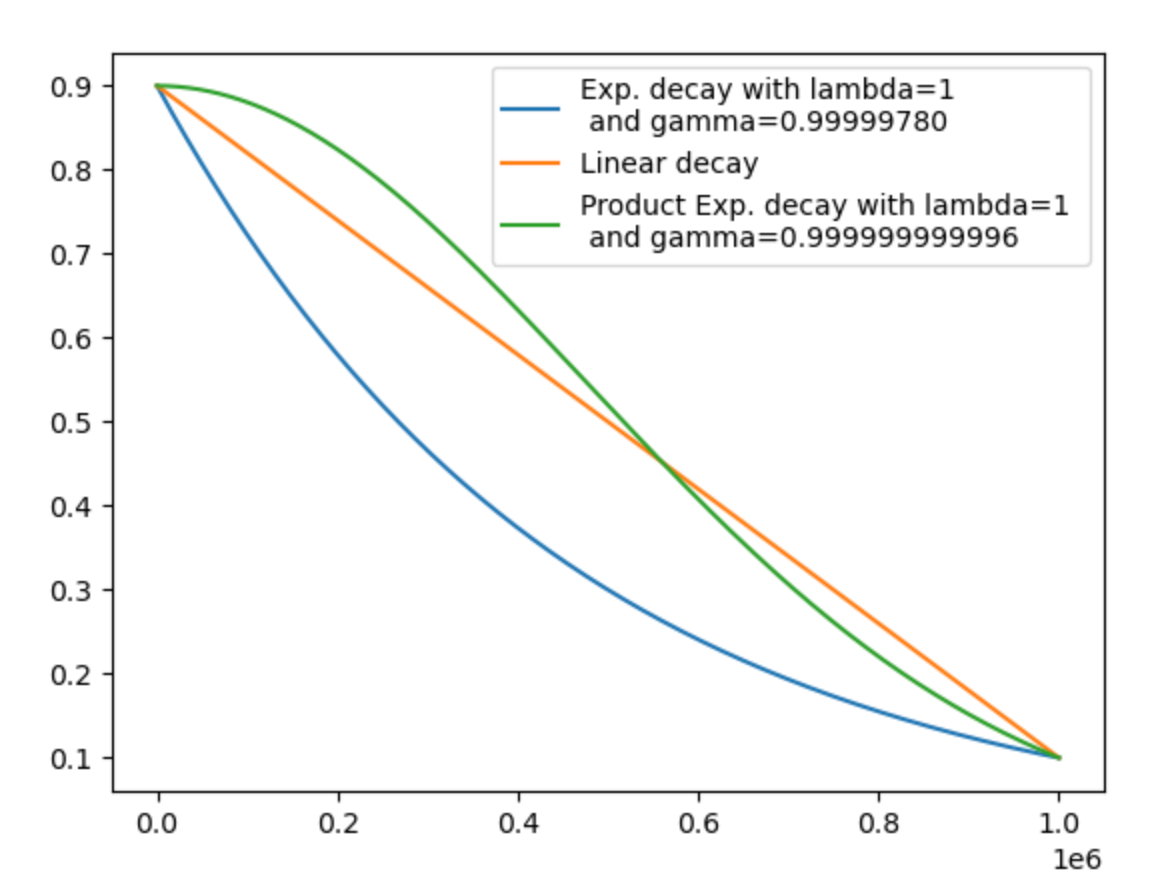
\includegraphics[width=0.7\linewidth]{figures/shape_exploration_functions}
	\caption{Shape of the proposed exploration functions for the DQN agent}
	\label{fig:shape_exp_funs}
\end{figure}

\subsection{Extracting explainability features}
In this section we are going to explain how, once we trained our models, we extracted several feature maps to understand what the model is taking into account to perform an action. We must note that for section \ref{sec:extracting_attn_maps}, we could not implement a way to extract raw attention maps for the SWIN transformer, nor we found any reference in the literature that would help us with this purpose, so we only extracted the attention maps for the ViT model. For section \ref{sec:grad_cam_act_maps}, the developed method takes into account both ViT and SWIN transformer.

\subsubsection{Extracting attention maps}
\label{sec:extracting_attn_maps}
As explained in section \ref{sec:vis-transformers}, the ViT introduces an additional token along the patches, called the class token, which holds the information that class takes into account via self-attention to produce the output. Figure \ref{fig:classtokenattention} illustrates this, since we can see that, for a 4 by 4 patched image, the disposition of the attention matrix for one attention head would give us for the class token row, all the patches with the weighted attention. The code developed for this section is available in the script \href{https://github.com/Javimh18/DL_TFM/blob/main/src/visualize_attention_vit.py}{visualize\_attention\_vit.py}.

\begin{figure}[!h]
	\centering
	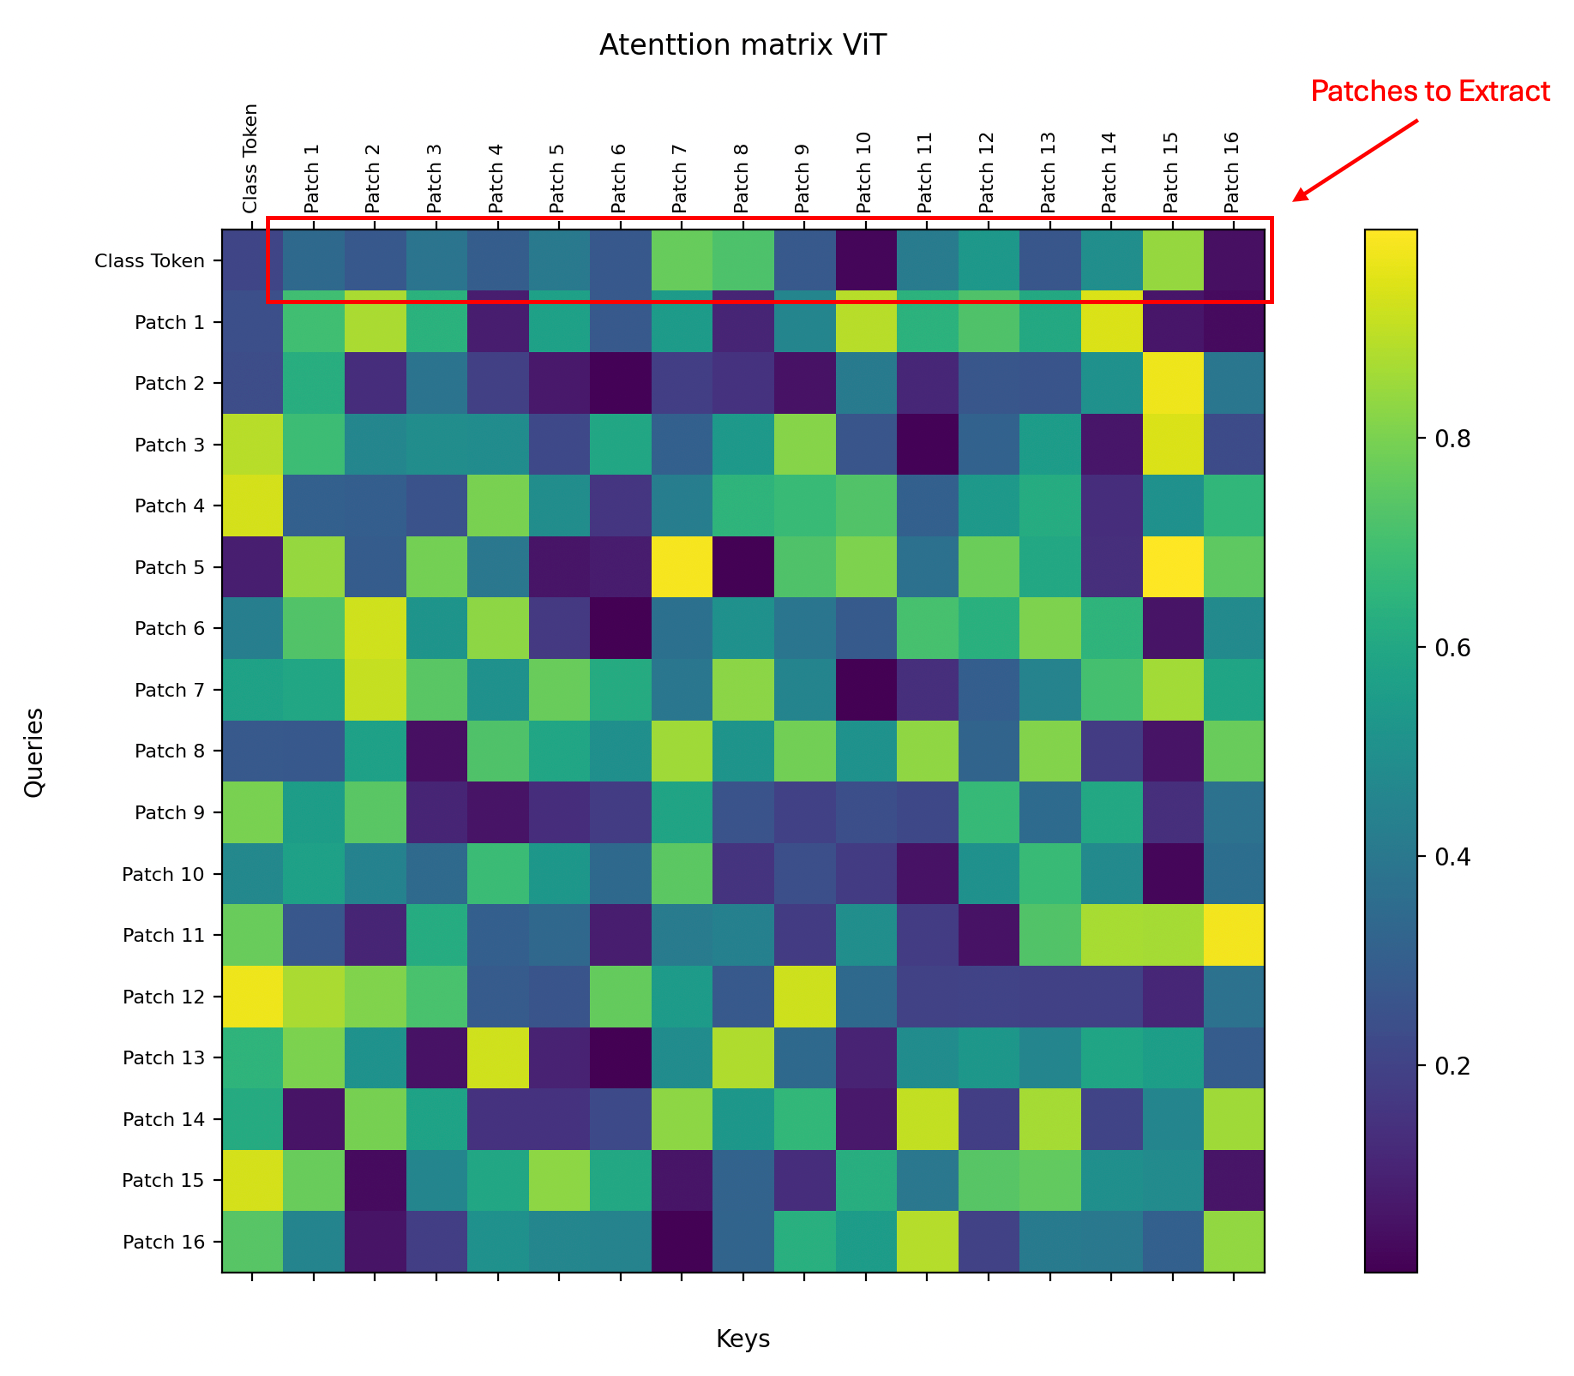
\includegraphics[width=0.7\linewidth]{figures/class_token_attention}
	\caption{Example of an attention matrix for one attention head with 4 $\times$ 4 patches. The section under the red rectangle refers to the patches that the class token ponders in order to perform the output. This patches will be our extraction for the attention maps.}
	\label{fig:classtokenattention}
\end{figure}

In order to extract the attention maps, the implementation from \cite{caron2021emerging} has the functionality of returning the attention maps in the forward pass of the ViT blocks (see listing \ref{code:attn_block}). The only thing we ought to do, is index the attention matrix correctly to extract the elements of interest. In listing \ref{code:single_frame_attn}, we can see a example of this. First, we obtain the attention weights for each patch by indexing the attention matrix like \inlinecode{attn[0, :, 0, 1:]} in line 3, obtaining a matrix with dimensions $\mathbb{R}^{nh \times (P-1)}$, where nh refers to the number of heads from the attention mechanism, and P refers to the tokens that go into the attention mechanism. Since we are not interested in the attention weight that the class token has with respect to itself, we exclude it out. To compute the averaged importance of each patch, we perform the mean across the nh dimension, and reshape the $P$ dimension to the original spatial dimensions $P_w$ and $P_h$ for the width and the height respectively (line 4). Then, by calling the method \inlinecode{interpolate_attn_map} we perform a interpolation to return the attention map to the original size of the input (lines 5 to 8).

\begin{lstlisting}[caption={Attention map extractor for a single frame}, label={code:single_frame_attn}]
	vit = agent.net.online
	attn = vit.get_last_selfattention(state.float())
	cls_attn = attn[0, :, 0, 1:]
	cls_attn = cls_attn.reshape(-1, dimension, dimension).mean(dim=0, keepdim=True).unsqueeze(0)
	# 3. Interpolate the attention maps to original frame size
	cls_attn_int = interpolate_attn_map(attention_map=cls_attn, 
	scale_factor=patch_size,
	final_shape=original_shape)
\end{lstlisting}

Once we have done this, we can plot the attention map along with the original frame to observe where does the model pay attention to, given a frame. In Figure \ref{fig:attnvisualizationframe} we provide an example for this. Additionally, in the right side of the figure, we provide the returned Q-values from the network, since they are of vital importance for understanding the network's decisions. The interpretations that we extract from this will be discussed in section \ref{cha:evaluation}.

\begin{figure} [!h]
	\centering
	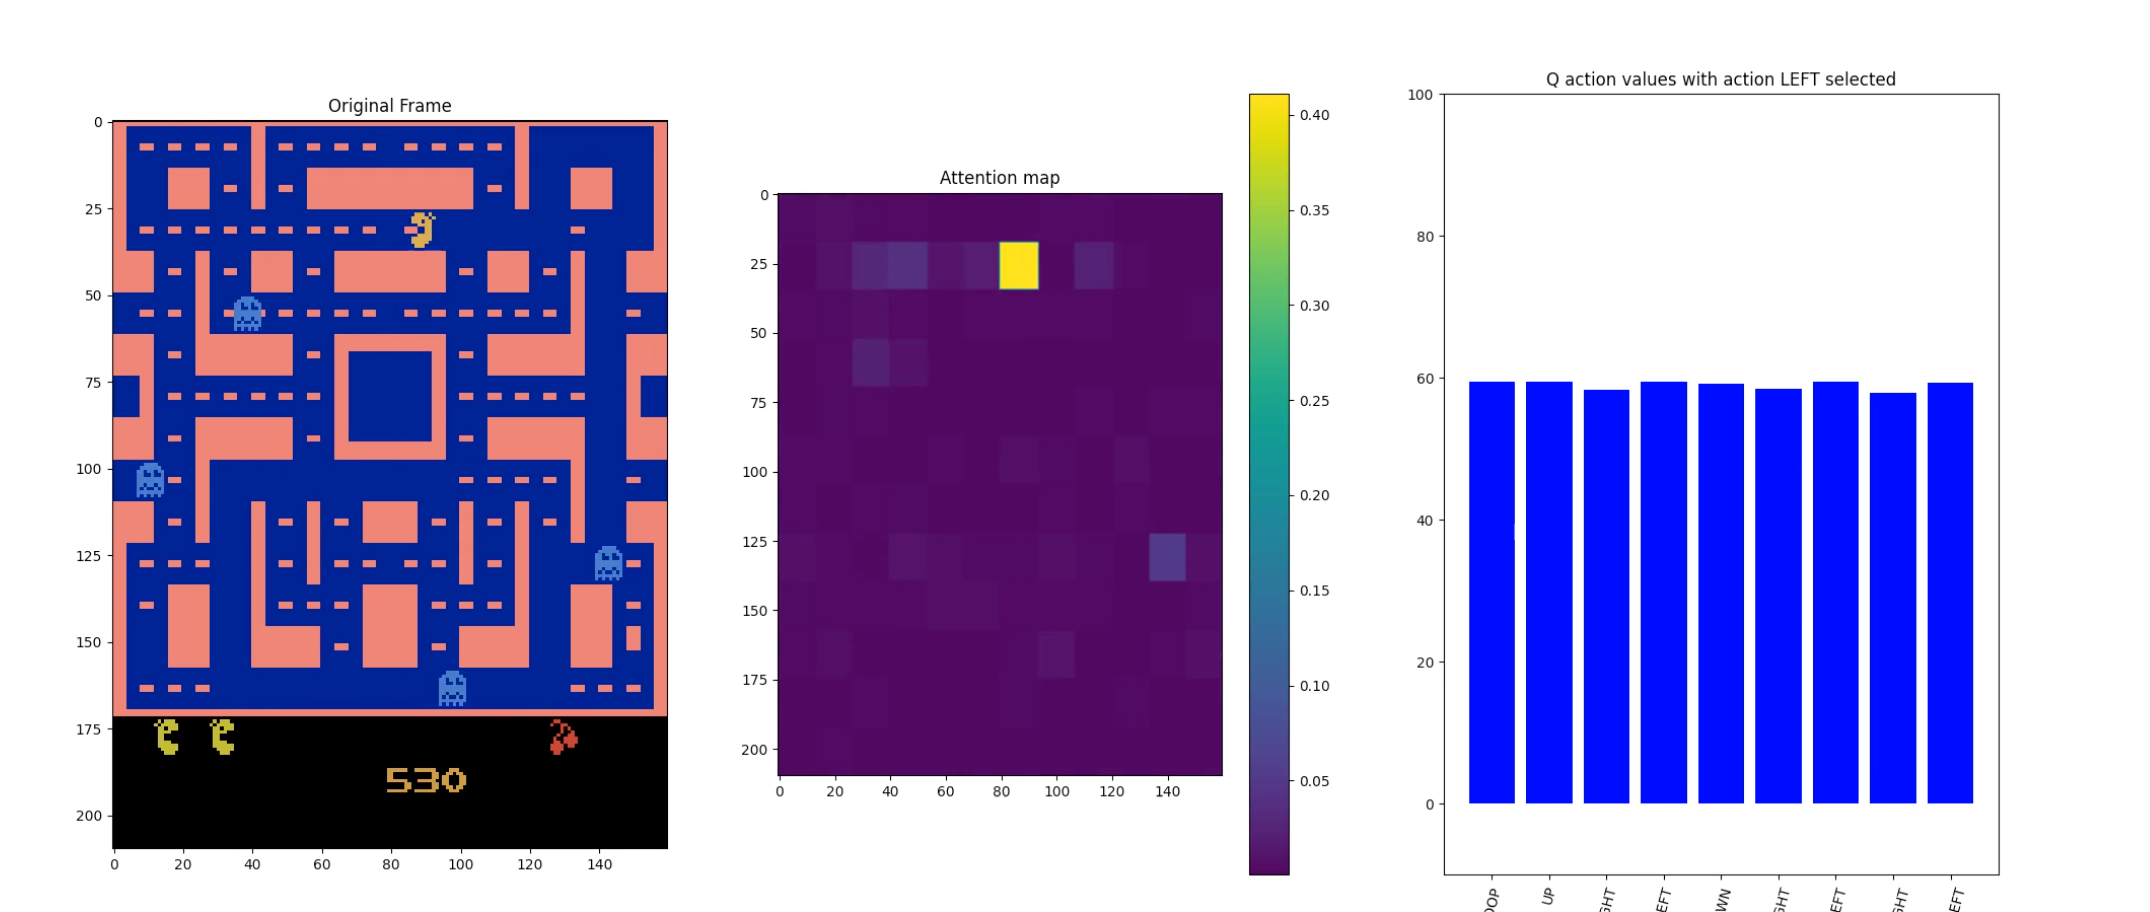
\includegraphics[width=\linewidth]{figures/attn_visualization_frame}
	\caption{Left side, the original frame from the game, in the center, the attention maps for the class token, at the right-side, the Q-values for the observation from the state.}
	\label{fig:attnvisualizationframe}
\end{figure}



\subsubsection{Extracting Grad-CAM's activation maps}
\label{sec:grad_cam_act_maps}
We developed something similar to section \ref{sec:extracting_attn_maps} but using the grad-CAM technique explained in \ref{sec:cam}. To do so, we used the \inlinecode{pytorch-cam} library \cite{jacobgilpytorchcam} that integrates a well varied amount of CAM methods to select. Part of the developed code is displayed in listing \ref{code:grad_cam_rl}, and the complete code can be found in the \href{https://github.com/Javimh18/DL_TFM/blob/main/src/visualize_activations.py}{visualize\_activations.py} script.

\begin{lstlisting}[caption={Activation maps using Grad-CAM}, label={code:grad_cam_rl}]
	action, q_v = agent.perform_action(state, t=-1, exploit=True)
	actions.append(action)
	q_values.append(q_v.squeeze().detach().cpu().numpy())
	# 2. get the activation maps
	state = first_if_tuple(state).__array__()
	state = torch.tensor(np.array([state]), device=device)
	action_target = ClassifierOutputTarget(action)
	gray_scale_cam = cam(input_tensor=state, targets=[action_target])
	gray_scale_cam = torch.tensor(gray_scale_cam[0, :]).unsqueeze(0).unsqueeze(0) # appropiate dims for interpolation
	activ_map = interpolate_activations(gray_scale_cam,
	final_shape=original_shape)
\end{lstlisting}

To adapt Grad-CAM from the classification supervised learning set-up to the reinforcement learning set-up, we treated each of the actions the agent selected as the predicted "class". By doing so, we expected to obtain the biggest activations from the input that the agent considers to perform the output. The \inlinecode{ClassifierOutputTarget} method takes the target class (our action in this case), and passes it to the cam method, that returns the activations. Then we perform an interpolation to return the resolution to the original frame size, obtaining a map depicted in Figure \ref{fig:activationmapsvisualization}. We must say that this method works for both ViT and SWIN backbones, along with other non-attention based models, such as CNNs. 

\begin{figure}[!h]
	\centering
	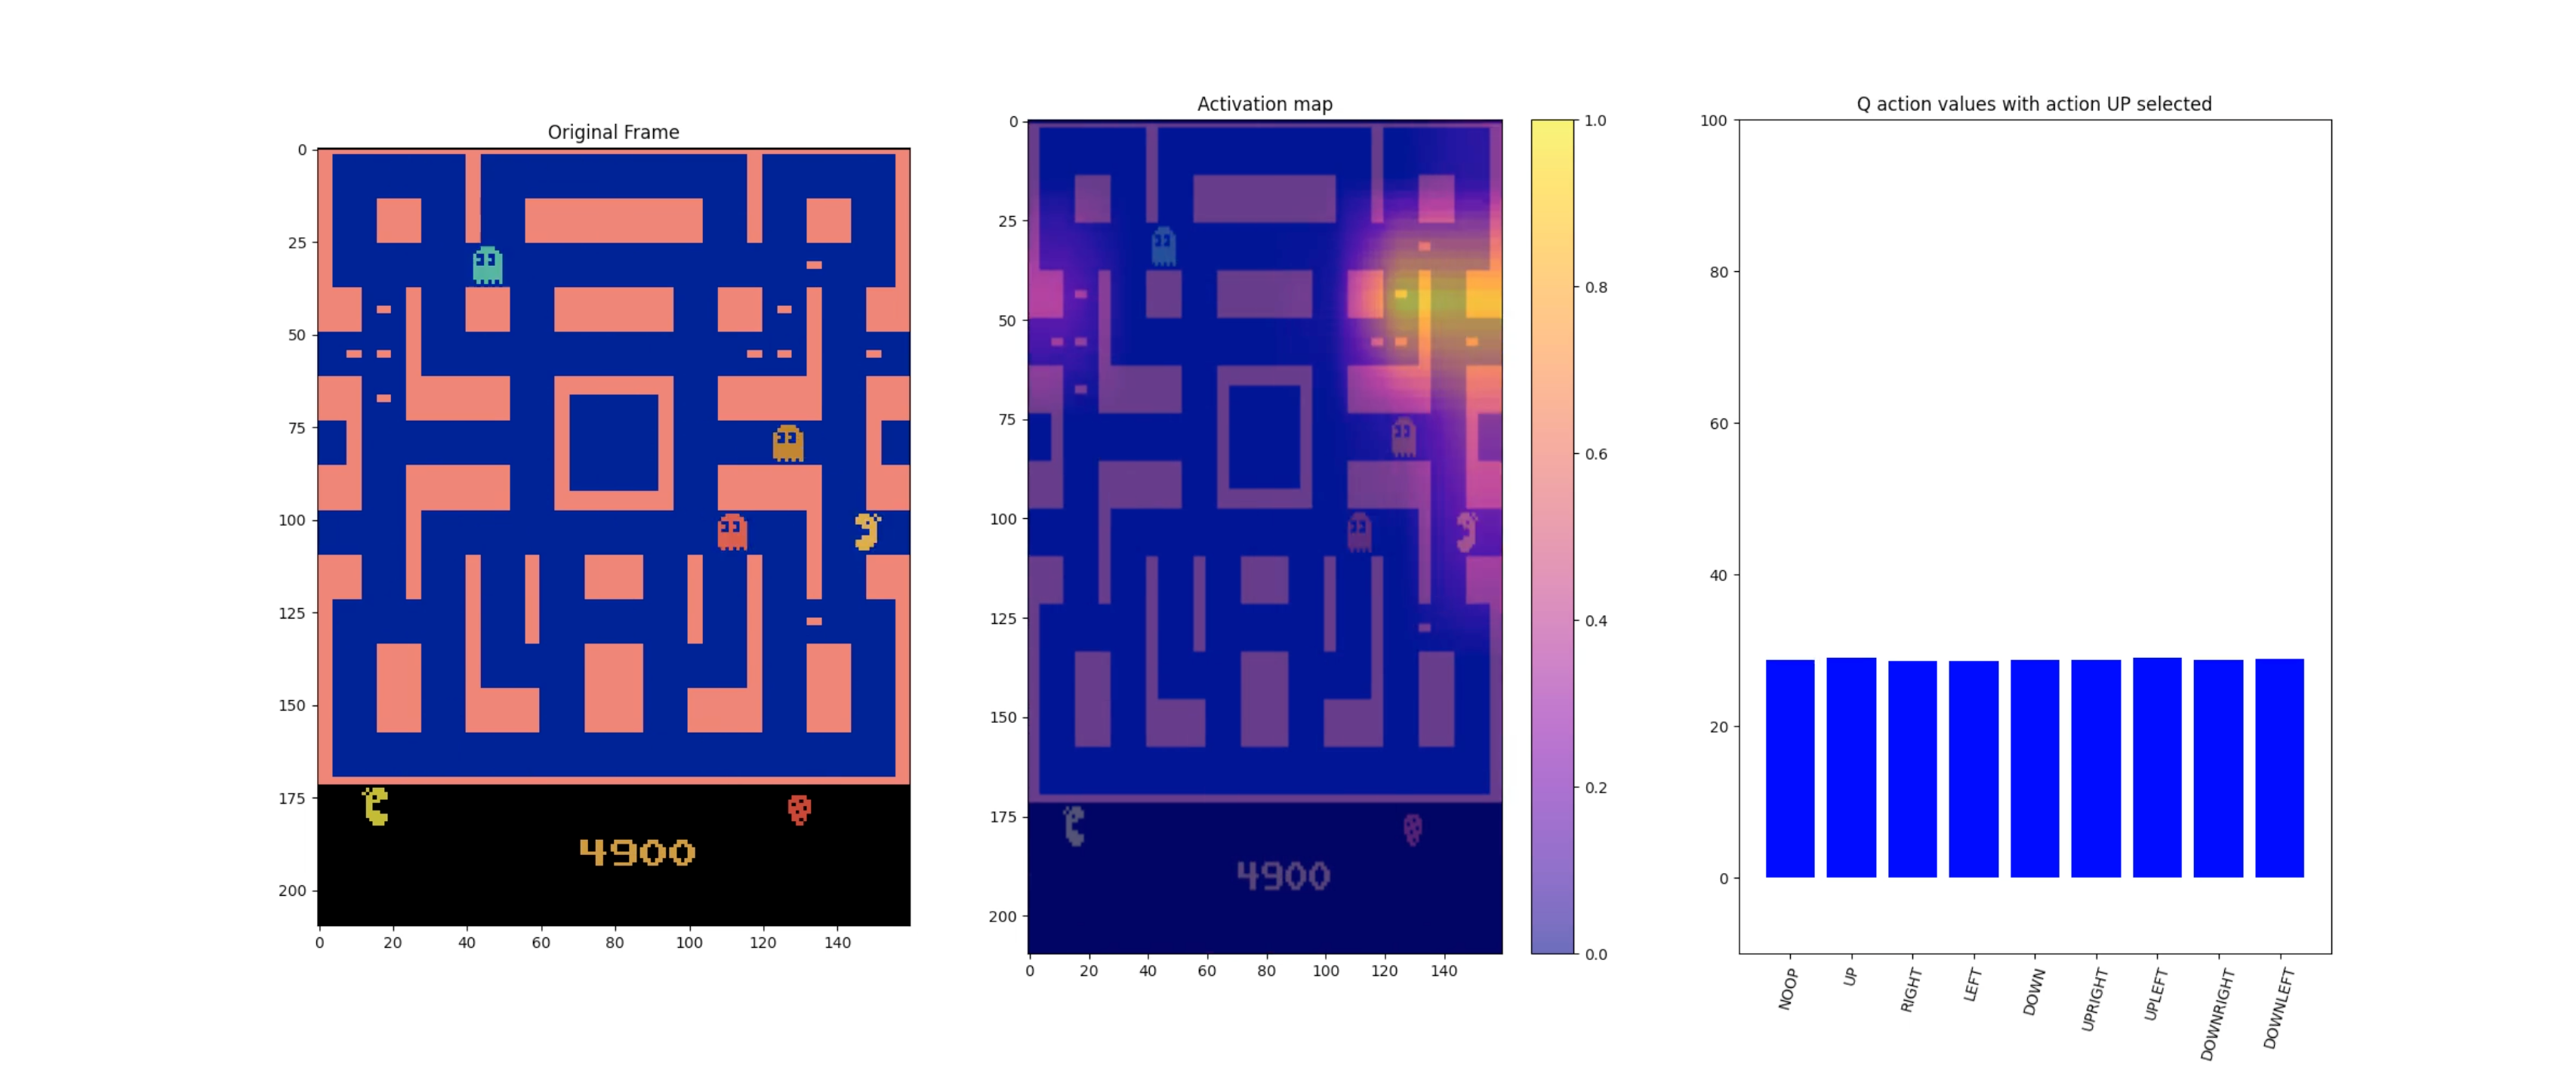
\includegraphics[width=\linewidth]{figures/activation_maps_visualization}
	\caption{Left-side, the current frame of the game. In the center, the activation maps from the ViT using grad-CAM. At the right-side, the Q-values provided by the neural network.}
	\label{fig:activationmapsvisualization}
\end{figure}


\subsection{Additional implementations}

\subsubsection{Configuration files}
As explained in sections \ref{sec:vit_transformer_imp} and \ref{sec:swin_transformer_rl}, the implementation of these models is highly parametrizable, since we can state lots of parameters that are involved in the topology of the models. Changing these parameters manually in each file is a burden, since we have to check that the changes are done correctly in the several files involved in running the training process. To tackle this issue, we proposed two files: one for the DQN agent hyper-parameters, and another for the models hyper-parameters called \href{https://github.com/Javimh18/DL_TFM/blob/main/config/agents_config.yaml}{agents\_config.yaml} and \href{https://github.com/Javimh18/DL_TFM/blob/main/config/agent_nns.yaml}{agent\_nns.yaml}.
For loading this files, we used the \inlinecode{pyyaml} library, that eases a lot the loading a manipulation of yaml files, and used them properly to initialize the corresponding hyper-parameters, such as number of steps for training, the learning rate for the back-propagation and the Q-estimates or the number of layers that our model will have. Thanks to this implementation, we were able to seamlessly change the configuration of the agents, allowing for room to explore different hyper-parameters configurations.

\subsubsection{Checkpoints}
As the training process progresses, the weights of our function approximators will change. There are some cases where the excess of training produces a degradation on the model's performance, ending the training with a sub-optimal model. To change this, we implemented a checkpoint saver in our pipeline, that saves periodically the model's state dictionary, that contains the weights of the model. By doing a snap-shot of the model weights, we have several versions, which will be of use when we run our evaluations of the agents in the environment. Additionally, the checkpoints are of great use if we want to resume a training process. We have also developed adaptations to our code that perform these kinds of operations, and have been of great use when unexpected events (such as lack of computational resources) stopped our training process.

\subsection{Overview}
\label{sec:overview_implementation}

With almost all the components involved in the training pipeline for our agents, in Figure \ref{fig:implementationoverview} we present the diagram of all the modules developed along with their relationships. 

\begin{figure}[!h]
	\centering
	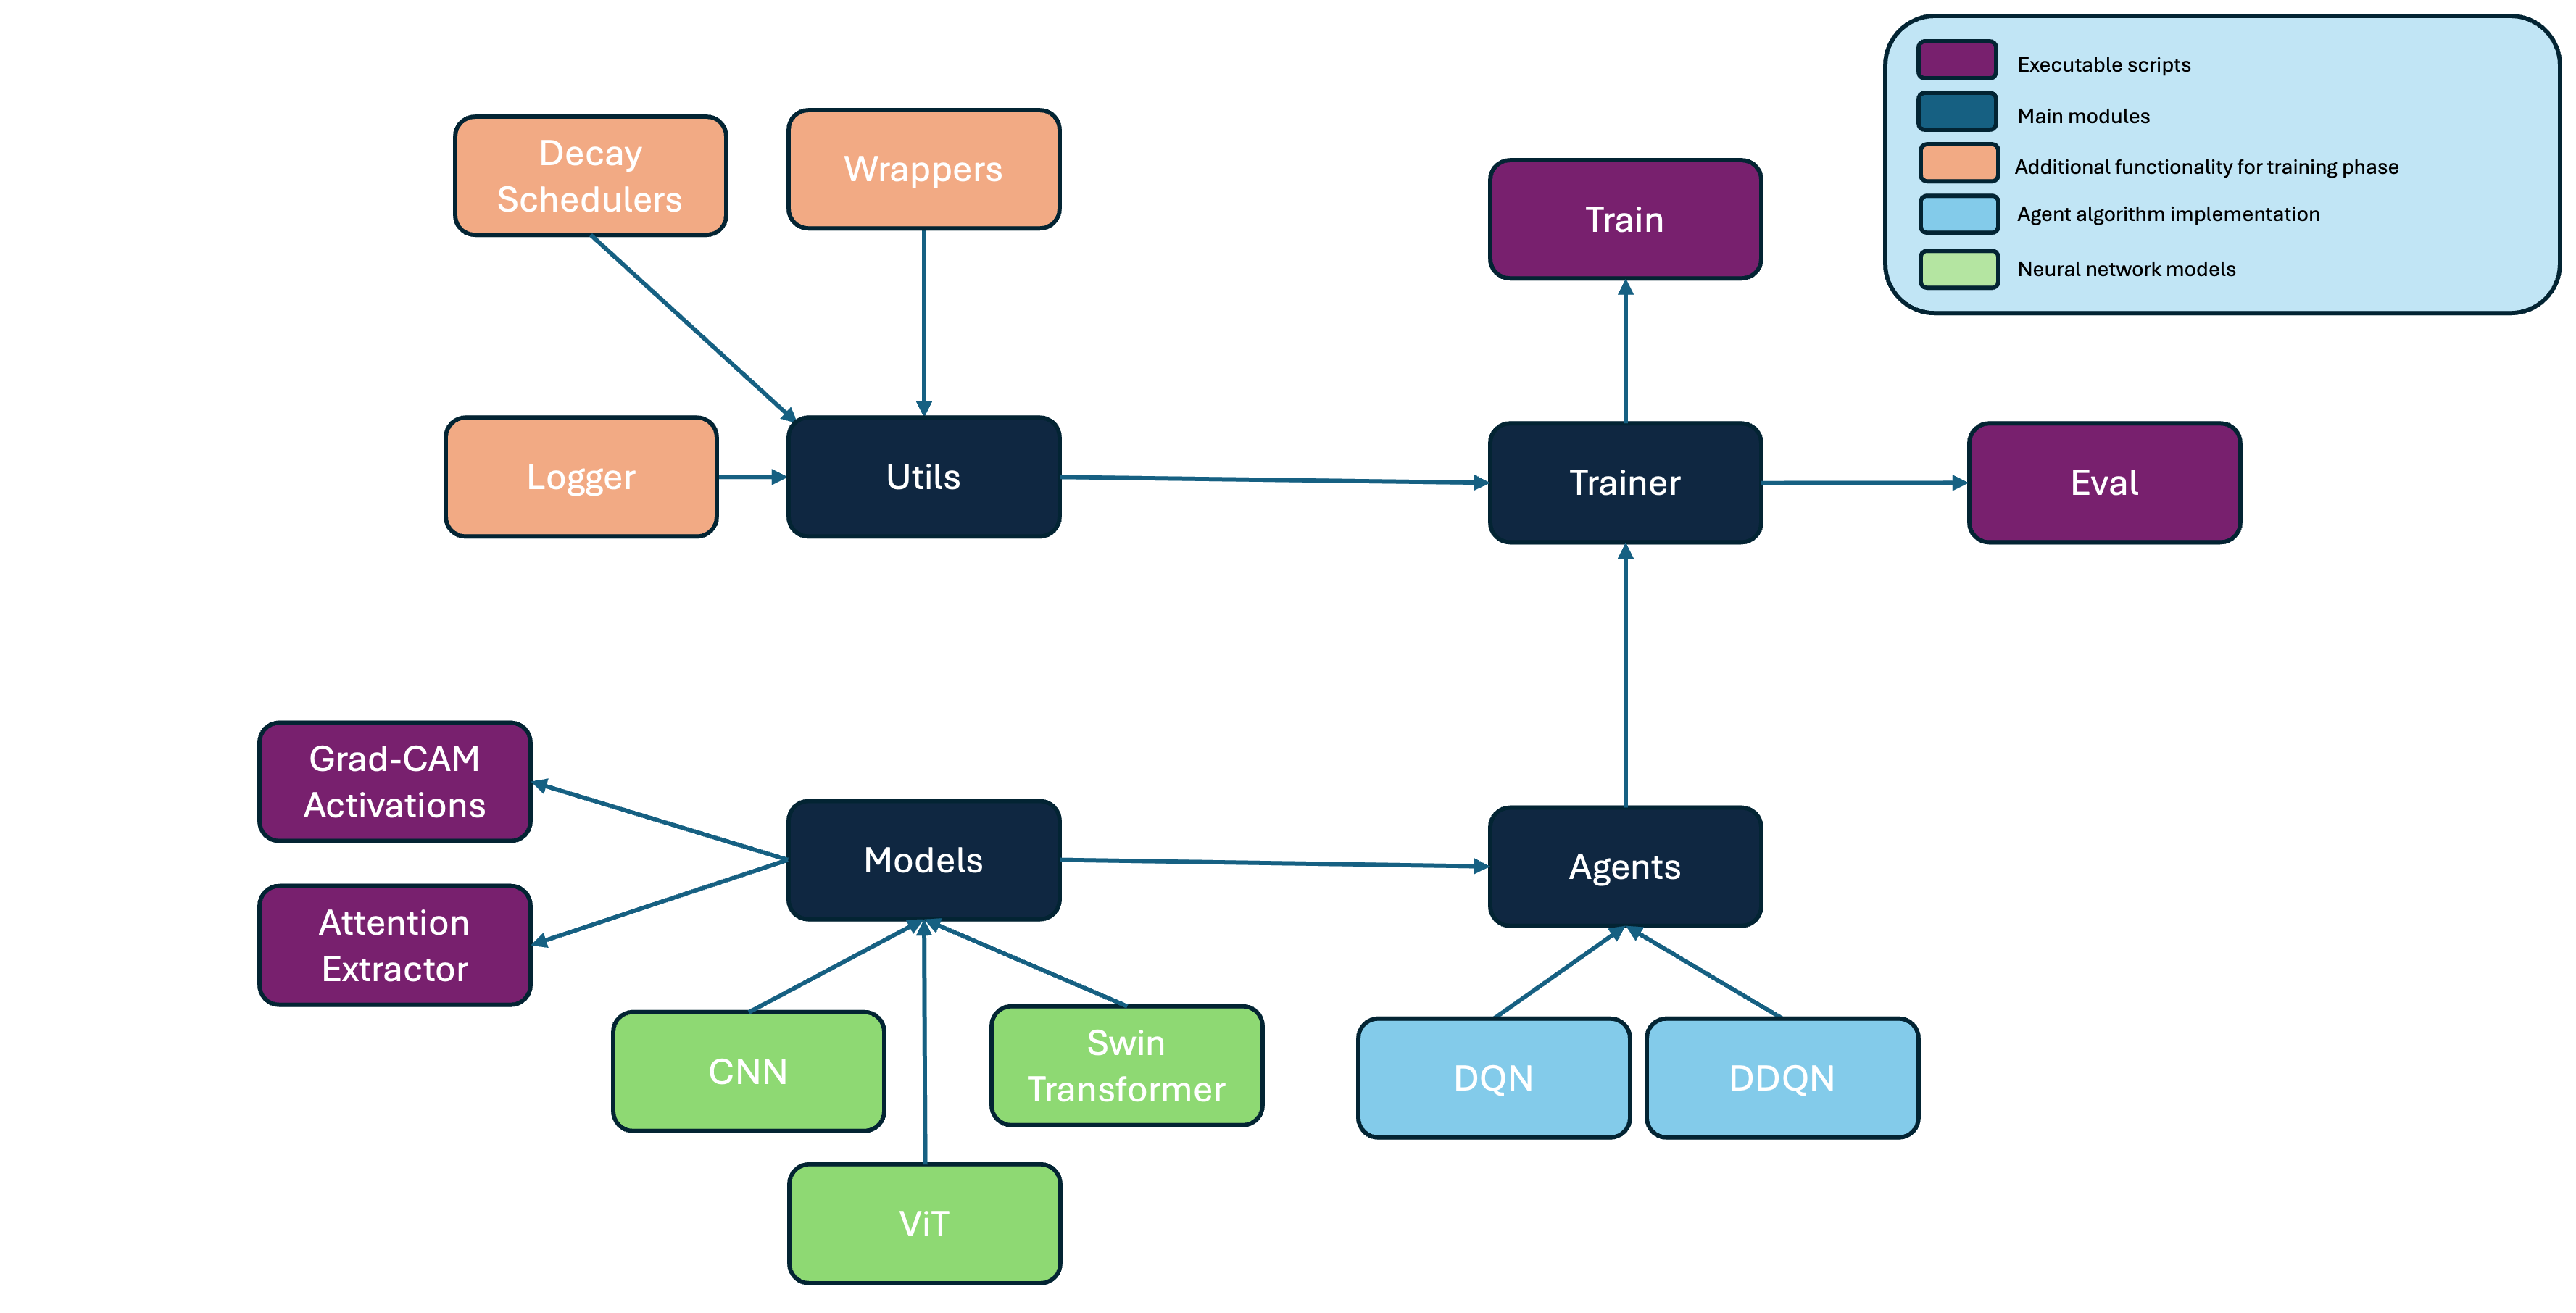
\includegraphics[width=\linewidth]{figures/implementationoverview}
	\caption{Implementation overview of all the modules involved in this work}
	\label{fig:implementationoverview}
\end{figure}





                  % incluir capítulo de diseño-y-desarrollo/design-and-development
\chapter{Evaluation}
\label{cha:evaluation}

\section{Experimental set-up}
\label{sec:exp_setup}

\subsection{Environments}
\label{sec:env_setup}

\subsection{Proposed models set-up}
\label{sec:models_setup}

\section{Joint Evaluation}
\label{sec:joint_ev}

\subsection{Attention and other markers for explainability}
\label{sec:joint_attn_explainability}

\subsection{Qualitative results}
\label{sec:joint_qual_explainability}

\subsection{Quantitative results}
\label{sec:joint_quant_explainability}

\subsection{Counter-examples}
\label{sec:counter_examples}

%
%\begin{table}[]
%	\begin{center}
	%		\caption[Sample table (short title)]{Sample table (long title)}
	%		\label{tab:sample-table}
	%		\begin{tabular}{||c c c c||} 
		%			\hline
		%			Col1 & Col2 & Col2 & Col3 \\ [0.5ex] 
		%			\hline\hline
		%			1 & 6 & 87837 & 787 \\ 
		%			\hline
		%			2 & 7 & 78 & 5415 \\
		%			\hline
		%			3 & 545 & 778 & 7507 \\
		%			\hline
		%			4 & 545 & 18744 & 7560 \\
		%			\hline
		%			5 & 88 & 788 & 6344 \\ [1ex] 
		%			\hline
		%		\end{tabular}
	%	\end{center}
%\end{table}

              % incluir capítulo de evaluacion/evaluation
%%%%%%%%%%%%%%%%%%%% CONCLUSIONES Y TRABAJO FUTURO / CONCLUSIONS AND FUTURE WORK CHAPTER %%%%%%%%%%%%%%%%%%%%%%
\chapter{Conclusions and future work}
\label{cha:conclusions}

\section{Conclusions}
...

\section{Future work}
...            % incluir capítulo de conclusiones/conclusions

\bibliographystyle{ieeetr}
\bibliography{bibliography}

\begin{appendices}
%%%%%%%%%%%%%%%%%%%% ANEXOS / APPENDIX %%%%%%%%%%%%%%%%%%%%%%
\appendix           % appendix starts from here
\appendixpage  		% add a blank page to start the appendix
\addappheadtotoc 	% add appendix to the TOC

\chapter{Reinforcement Learning}
\label{chap:appendix-c1}

\section{Classic learning methods in RL} \label{app:classic_rl}
\subsection{Monte Carlo estimation:} 
Monte Carlo estimation \cite{gerstner2021multilevel} uses complete episodes to approximate the value function using the empirical mean. The value function is based on the returns $G_t$, and since we are trying to approximate $V_{\pi}(s)$, our returns will be the statistic we will use to adjust the value of a state $S_t$. In non-stationary problems, where the environment may change over time, the value function will be incrementally updated as in equation \ref{eq:eq_mc_update}, and by the law of large numbers, if the number of times we visited a state $S$ goes close to infinity, then $V(S) = V_{\pi}(S)$ 

\begin{equation} \label{eq:eq_mc_update}
	V(S_t) \leftarrow V(S_t) + \alpha(G_t - V(S_t))
\end{equation}

Where $\alpha$ is the step-size hyper-parameter that tells the update function how much error take into account in the when performing the adjustments from the estimates. This approach has unbiased but noisy estimations, as the rewards distribution may not be consistent between episodes, creating prone-to-error estimates that may take a long time to converge to the true value function $V_{\pi}(s)$.

\subsection{Temporal Difference Learning:}
TD methods learn from episodic and non-episodic experiences, so the concept of bootstrapping is introduced. Bootstrapping refers to the ability of a model to make an approximation of the value function every each \textit{n-steps}, using the estimation of the returns we have computed as we have collected more and more experience without finishing the current episode. The simplest set-up of TD is TD(0), where we look ahead only one time-step, from $S$ to $S_{t+1}$, and the update for the value function is defined in equation \ref{eq:eq_td0_update}.

\begin{equation} \label{eq:eq_td0_update}
	V(S_t) \leftarrow V(S_t) + \alpha(R_{t+1} + \gamma V(S_{t+1}) - V(S_t))
\end{equation}

Why is this a good idea? imagine a situation where an agent is driving a car, and another car comes towards the agent, but avoids it in the last moment. In the Monte Carlo learning approach, as it learns from complete episodes, the agent would not have learned anything, since the episode ended without much consequences. In TD(0), since it is learning from each time-step, the agent would have learn from the experience itself, and for example, discover that, when a car is approaching, slowing down to have better maneuverability could be an great approach.

Looking just one step in the future might be a little short-sighted, so we can consider to look several steps ahead, considering:

\begin{itemize}
	\item For n = 1 $\rightarrow G^{1}_t = R_{t+1} + \gamma V(S_{t+1})$
	\item For n = 2 $\rightarrow G^{2}_t = R_{t+1} + \gamma R_{t+2} + \gamma V(S_{t+1})$
	\item For n = k $\rightarrow G^{k}_t = R_{t+1} + \gamma R_{t+2} ... \gamma^{k-1}R_{t+k} + \gamma^{k} V(S_{t+k})$
\end{itemize}

What we may not know which n is better, since the search space can be infinite. So the solution that TD($\lambda$) proposes is to have a weighted sum of the returns taking into account different time horizons (equation \ref{eq:lamda_return}), and then use it as our estimation of the value as portrayed in update equation \ref{eq:tdlambda_update}. Figure \ref{fig:td_returns} portrays a visual illustration of how this works.

\begin{equation}\label{eq:lamda_return}
	G^{\lambda}_{t} = (1-\lambda)\sum_{n=1}^{k} \lambda^{n-1}G^{n}_{t}
\end{equation}

\begin{equation} \label{eq:tdlambda_update}
	V(S_t) \leftarrow V(S_t) + \alpha(G^{\lambda}_{t} - V(S_t))
\end{equation}

A few things to comment about the TD($\lambda$) equation is that if $k=\infty$, then we would be in a similar to Monte Carlo learning update, but if $k=1$, then we would end up in the TD(0) update equation.

\begin{figure}[!h]
	\centering
	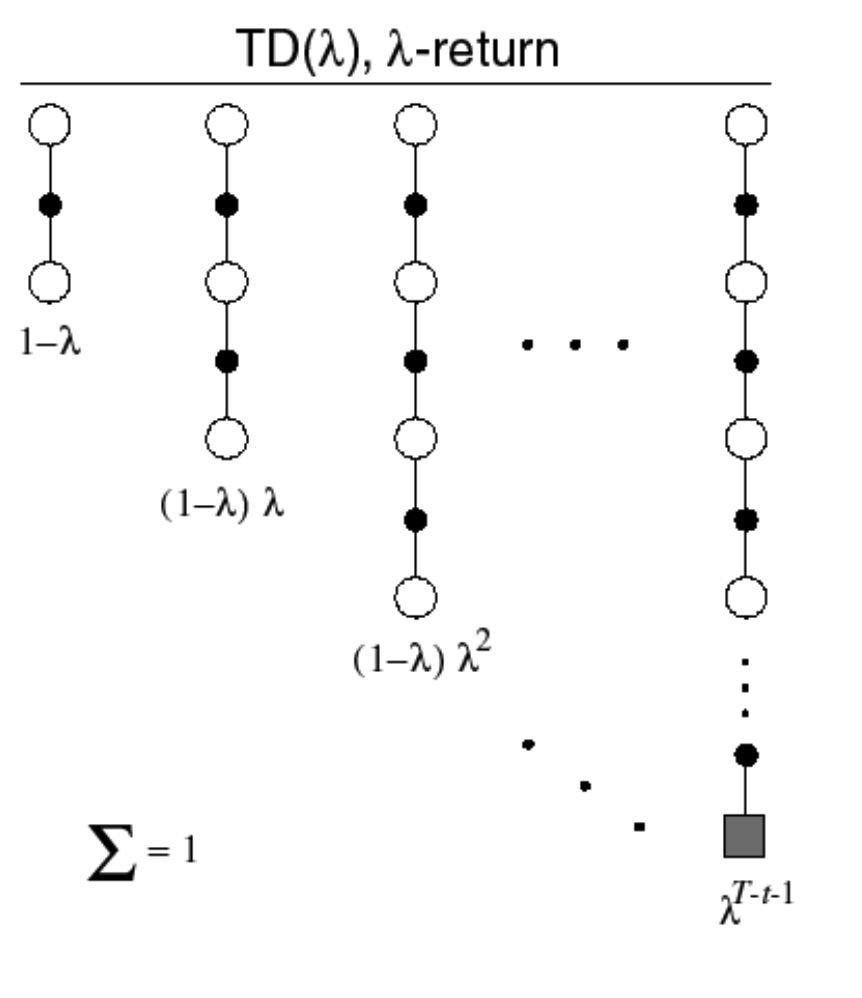
\includegraphics[scale=0.5]{figures/tdlambda_return.png}
	\caption{TD Returns}
	\label{fig:td_returns}
\end{figure}

The policy will use these values to act greedily, as defined in equation \ref{eq:eq_greedy_policy}. Since what it wants to maximize is the value, given the MDP model and the action space $\mathcal{A}$, the policy will select the action that gives more value in future states s'. The issue is that, as stated at the beginning of this section, we are in model-free RL and we no longer have the environment dynamics and $\mathcal{P}$ and reward function $\mathcal{A}$. In the next section we will introduce control, and with it, how the policy problem in tackled.

\begin{equation} \label{eq:eq_greedy_policy}
	\pi'(s) = \operatorname*{argmax}_{a \ni \mathcal{A}} \mathcal{R}^{a}_{s} + \mathcal{P}^{a}_{ss'} V(s')
\end{equation}

\subsection{On-Policy Control: } \label{app:on-policy-control}

On policy RL means that the updates of the value functions are performed according to following a policy $\pi$. Up until this point, everything we have done is evaluate states, and act according to those values. The issue is, that the policy defined in equation \ref{eq:eq_greedy_policy} requires a model of the MDP, and since we are in model-free RL, this is not possible. Instead, we introduce action-value functions, $Q(s,a)$ that take into account, the value of an action, given a state (equation \ref{eq:q_value}).

\begin{equation} \label{eq:q_value}
	q_{\pi}(s,a) = \mathbb{E}_{\pi}[R_{t+1} + \gamma q_{\pi}(S_{t+1},A_{t+1}) | S_t=s , A_t=a]
\end{equation}

Now, we re-write the policy in equation \ref{eq:action_value_policy}, that it still greedy, since we pick the action a that maximizes the action value estimates $Q$, given a state s.

\begin{equation} \label{eq:action_value_policy}
	\pi'(s) = \operatorname*{argmax}_{a \ni \mathcal{A}} {Q}(s,a)
\end{equation}

One thing to note is that, if our policy always acts greedily, then it will never explore other states, since it will always prioritize rewards over landing on new states that may lead to biggest rewards. This is why the $\epsilon$-greedy policy was introduced. This policy acts greedily with a probability of $p = (1 - \epsilon)$ and randomly with a probability $p = \epsilon$. 

Since now we are dealing with action-value functions, we must adapt the TD algorithm. This adaptation is the SARSA algorithm (State-Action-Reward-State-Action) and its update function is shown in equation \ref{eq:sarsa}.

\begin{equation} \label{eq:sarsa}
	{Q}(S,A) \leftarrow {Q}(S,A) + \alpha(R + \gamma{Q}(S',A') - {Q}(S,A))
\end{equation}

\noindent where we define the TD error in equation \ref{eq:td_error}.
\begin{equation} \label{eq:td_error}
	\delta = R + \gamma{Q}(S',A') - {Q}(S,A)
\end{equation}

If we take the approach of TD($\lambda$), we can use SARSA as a along a n-step action-value estimator, instead of just one look-ahead estimator. 

\begin{itemize}
	\item For n = 1 $\rightarrow q^{1}_t = R_{t+1} + \gamma Q(S_{t+1})$
	\item For n = 2 $\rightarrow q^{2}_t = R_{t+1} + \gamma R_{t+2} + \gamma Q(S_{t+1})$
	\item For n = k $\rightarrow q^{k}_t = R_{t+1} + \gamma R_{t+2} ... \gamma^{k-1}R_{t+k} + \gamma^{k} Q(S_{t+k})$
\end{itemize}

And using the same weighted average using the $\lambda$ parameter, we can obtain the SARSA($\lambda$) algorithm, as shown in equation \ref{eq:sarsa_lambda_return}

\begin{equation}\label{eq:sarsa_lambda_return}
	q^{\lambda}_{t} = (1-\lambda)\sum_{n=1}^{k} \lambda^{n-1}q^{n}_{t}
\end{equation}

\begin{equation} \label{eq:sarsa_lambda}
	{Q}(S_t,A_t) \leftarrow {Q}(S_t,A_t) + \alpha(q^{\lambda}_{t} - {Q}(S_t,A_t))
\end{equation}

\subsection{Off-Policy Control: } \label{app:on_policy_control}

Dealing with just one policy, $\pi$, may limit the scope of learning. To put a easy example, it would be as if humans would only learn following a single philosophy. It is not a bad approach, but as we add new perspectives to our learning process, better outcomes come out of it (i.e. work, university, relationships). Off-policy learning, among other motives, was introduce to make the agent more flexible in the learning process, taking into account different perspectives and explore while learning the optimal policy. In off-policy learning, usually there are two policies: the target policy $\pi$ that is used to compute the ${Q}$ values, and the behavioural policy $\mu$, which usually has an exploratory component to it.

One of the most famous algorithms that implements off-policy learning is Q-learning \cite{Watkins1992}. It is mainly divided in three blocks:

\begin{enumerate}
	\item The next action $A_{t+1}$ is selected following the behaviour policy $\mu(A|S_t)$
	\item The alternate action A' is selected following the target policy $\pi(A|S_t)$
	\item Use the update equation (eq. \ref{eq:q_leaning}) to update the action-values ${Q}$.
\end{enumerate}

\begin{equation} \label{eq:q_leaning}
	{Q}(S_t, A_t) \leftarrow {Q}(S_t, A_t) + \alpha[R_{t+1} +  \operatorname*{max}_{a'}\gamma{Q}(S_{t+1}, a') - {Q}(S_t, A_t)]
\end{equation}

\subsection{Actor-Critic Methods}
\label{sec:ac-methods}
Currently, the most common policy gradient methods are based on actor-critic methods. The critic (action-value function) makes evaluations of the actor's actions using function approximation $\hat{{Q}}_{w}(s,a)$. The actor tries actions and optimize them in the direction the critic proposes. This is formalized in equation \ref{eq:actor-critic} where the approximation of the policy gradient takes into account the action-value function as part of the update.

\begin{equation}\label{eq:actor-critic}
	\Delta\theta_{t} = \alpha(\nabla_{\theta} log \pi_{\theta}(s,a)\hat{{Q}}_{w}(s,a))
\end{equation}

One thing to note is that in this method we have two approximators, hence, two set of parameters, w and $\theta$. The most recent actor critic methods follow this principle, but add different optimization tools to obtain more stable and robust results in the policy learning process.

\begin{itemize}
	\item Soft Actor-Critic (SAC) \cite{haarnoja2018soft}: SAC is another off-policy actor-critic algorithm that incorporates maximum entropy reinforcement learning. It maximizes the expected return while also maximizing entropy, leading to policies that are more exploratory and robust. Right now is the state-of-the-art method for policy optimization.
	\item Proximal Policy Optimization (PPO) \cite{schulman2017proximal}: PPO is an actor-critic method that addresses the limitations of previous policy gradient methods. This is done by limiting the policy update to be close to the previous policy, helping to stabilize training and preventing large policy updates which may lead to performance degradation.
	\item Deep Deterministic Policy Gradient (DDPG) \cite{lillicrap2019continuous}: DDPG is an off-policy actor-critic algorithm specifically designed for continuous action spaces. This are spaces where the set of actions may be infinte, and a greedy (max) policy do not work. It learns a deterministic policy function using deep neural networks to approximate the Q-function and the policy.
\end{itemize}

\chapter{Attention Mechanism}

\section{Understanding the attention mechanism}
\label{app:attention-mec}

The attention mechanism appeared as a learnable alignment method for the translation task. This sequence to sequence problem had a weakness in the recursive neural network set-up. Up until that point, the way this kind of problem was addressed was by using a bidirectional RNN (usually a bi-LSTM) in the encoder, that tried to compress the information from the whole sequence in the hidden state vector from the LSTM. This was done forward and backwards to then concatenate the hidden state vectors from both LSTMs into one joint vector. This is defined in equation \ref{eq:bi_hidden_vector}

\begin{equation}
	\label{eq:bi_hidden_vector}
	\textbf{h}_1, ..., \textbf{h}_t = \text{bi-RNN}(x_1, ..., x_t)
\end{equation}

where $\textbf{h}_i$ is computed like shown in equation \ref{eq:h_vector}, where the notation $\{\cdot ; \cdot\}$ represents the concatenation between two vectors.

\begin{equation}
\begin{split}
	\label{eq:h_vector}
	\overrightarrow{h_i} = RNN_{forward}(x_i) \\
	\overleftarrow{h_i}  = RNN_{backward}(x_i) \\
	\textbf{h}_i = \{\overrightarrow{h_i};\overleftarrow{h_i}\}
\end{split}
\end{equation}

After that, the encoder, usually another RNN, would use the joint vector  $\textbf{h}_i$ to "decode" the sequence into the desired output (i.e.  the translated version of the input). As one could sense, compressing the information of big sequences becomes a problem when the hidden vector is of fixed size. What the attention mechanism proposed, was a way to dynamically change the hidden vector as the sequence was processed and new context from the input was acquired.

Bahdanu \textit{et al.} used the same set-up in the encoder in \cite{bahdanau2016neural}, but introduced new modifications at the decoder to make the hidden vector change over the time-steps of the sequence. To do so, they introduced the attention block, where the context vector $\textbf{c}_t$ is computed for each time step \textit{t}. This vector represents the relationship between the current output symbol and each term that belongs to the input sequence. Details on how the context vector $\textbf{c}_t$ is computed are at equation \ref{eq:context_vector_comp}

\begin{equation}
	\label{eq:context_vector_comp}
	c_t = \sum_{j=1}^{T} \alpha_{tj} \cdot \textbf{h}_j
\end{equation}

Where $\alpha_{tj}$ is a scalar that represents the weight of the hidden state vector $ \textbf{h}_j$ over the final context vector in time-step t. As one can interpret from equation \ref{eq:context_vector_comp},  $\alpha_{t}$ contains the information for all the input tokens processed up to the j-th element, hence, it will change its values for each time-step. Also, to prevent the decoder to "look ahead" of the sequence, the inputs tokens that are after the  j-th element in the sequence will be masked, so that the attention block cannot take them into account. The computation of  $\alpha_{tj}$ is showed in equation \ref{eq:weigth_comp}, where $s_{t-1}$ is the hidden state of the decoder at time-step t-1 and $f$ is a learnable function (i.e. a neural network) that outputs the logit (or energy, as they call it in the original work) $e_{tj}$, that ponders how much correlation exists between vectors $h_j$ and $s_{t-1}$. This correlation is then normalized by using the softmax function, producing the value $\alpha_{tj}$.

\begin{equation}
	\label{eq:weigth_comp}
	\begin{split}
		\alpha_{tj} = \frac{\text{exp}(e_{tj})}{\sum_{k=1}^{T} \text{exp}(e_{tk})} \\
		e_{tj} = f(s_{t-1}, h_j)
	\end{split}
\end{equation}

Finally, after all the alignments are computed, the RNN from the decoder outputs the most probable symbol $y_t$ at the current time-step $t$ (equation \ref{eq:dec_out_probs}).

\begin{equation}
	\label{eq:dec_out_probs}
	\mathbb{P}(y_t | y_{t-1}, ..., y_1, x) = RNN_{decoder} (c_t)
\end{equation}

\section{From attention to self-attention}
\label{from_att_2_selfatt}
Results from the attention encoder decoder architecture were a leap of performance with respect to previous work, but they still failed to perform correctly as the number of tokens in the input sequence increased. To tackle this problem, Vaswani \textit{et al.} proposed a different approach. Instead of the neural network processing one token at each time-step and compressing the information in a single hidden state vector iteratively, the sequence is processed as a whole, and each of the input tokens compute how relevant the other tokens are with respect to themselves. This mechanism is called self-attention.

To implement this mechanism, the authors propose to operate with three terms, the query Q, the keys K and the values V. These values are computed by projecting the original embeddings from the input $X \in \mathbb{R}^{n \times d}$, where n is the number of tokens in the input sequence and d is the embedding dimension, to the three matrices such that $Q = XW^Q$, $K = XW^K$ and $V = XW^V$. For clarification, $W^Q, W^K$ and $W^V \in  \mathbb{R}^{d \times d_k}$, where $d_k$ represents the dimension of the new space where $X$ is projected to compute $Q, K$ and $V$.

To follow the same terminology used in section \ref{app:attention-mec}, we are going to dissect the compact form of the attention defined in equation \ref{eq:app_self_attn} into the several parts so that resembles the way that the "classic" attention mechanism is computed.

\begin{equation}
	\label{eq:app_self_attn}
	\text{Attention}(Q, K, V) = \text{softmax}\left(\frac{QK^\top}{\sqrt{d_k}}\right) V
\end{equation}

In section \ref{app:attention-mec} we explained how the context vector $c_j$ contained the compressed information of the pondered sum from all the input tokens up to the j-th element of the sequence. On a similar fashion, the self-attention mechanism computes the context vector by projecting the j-th token of the input sequence, $x_j$, into a new space using $W^V$ and then pondering it with respect to the rest of the i-th elements from the sequence by multiplying them times $\alpha_{ij}$. As in the "classic" attention, $\alpha_{ij}$ is the normalized correlation between the i-th element and the j-th, and it is done by applying the softmax function, as shown in equation \ref{eq:self_attn_weigth_comp}, but the way $e_{i\cdot}$ is computing differs.

\begin{equation}
	\label{eq:self_attn_weigth_comp}
	\begin{split}
		\alpha_{ij} = \frac{\text{exp}(e_{ij})}{\sum_{k=1}^{n} \text{exp}(e_{ik})}
	\end{split}
\end{equation}

To compute the $e_{i\cdot}$ the self-attention formula proposes the scaled-dot product as the compatibility function. This function aims to give a magnitude of how correlated are two vectors from the input, since the dot product is greater the closer two vectors are on an euclidean space. Following this principle, we assume that the tokens that are similar semantically, will be closer in the embedding space, thus producing a greater value. The "scaled" part (i.e. $\frac{1}{\sqrt{d_z}}$)tries to stabilize the softmax function in terms of saturation, by preventing the values of the vectors from getting too big. This function is showed in equation \ref{eq:com_function_self_attn}, where $\cdot$ represents the dot-product between the i-th element in the query space and the j-th element in the key space, projected by the matrix-vector multiplication of their respective query and key projection matrices.

\begin{equation}
	\label{eq:com_function_self_attn}
	e_{ij} = \frac{(x_i W^Q)\cdot(x_j W^K)}{\sqrt{d_z}}
\end{equation}

Finally, to compute the attention-pondered final values $z_i$, we will multiply the weight values $\alpha_{ij}$ by each of the elements of the input $X$ after they are projected into the value space. Finally, we add them up, hence obtaining equation \ref{eq:final_attn_weights}.

\begin{equation}
	\label{eq:final_attn_weights}
	e_{ij} = \sum_{j=1}^{n} \alpha_{ij}(x_j) W^V
\end{equation}

As a final reflection, if we pay a closer look to equations \ref{eq:weigth_comp} and \ref{eq:com_function_self_attn}, we see that the mechanism is practically the same, where $h_i$ are the keys, and $s_{t-1}$ are the queries and the operations between them are practically the same, since $h_i$ and $s_{t-1}$ are the encoded information from the sequence in the embedded space. Something similar occurs with equations \ref{eq:final_attn_weights} and \ref{eq:context_vector_comp} where the value matrix is equivalent the $h_j$ vector at the input of the decoder. Here we can see that the relationship between the attention decoder and the self-attention mechanism from the transformer model lie under the same principles, compute which parts of the input are more relevant in terms of context to produce the appropriate output.


\chapter{Attention-models code analysis}
\label{cha:attn_models_code_analysis}

\section{Attention-based models: Vision Transformer}
\label{sec:vit_transformer_imp}
The aim of this work is to test out if there is any explain-ability in the decision making that agents perform when the value function is an approximator, which is an ideal set-up for DQN learning. For this section we will discuss the implementation of the attention-based models (i.e. vision transformers) that were used to carry out our experiments. First, we will talk about the Vision Transformer, discussing about the relevant aspects involved from the intuition to the actual implementation, that we took from \cite{caron2021emerging}. 

In several implementations for the vision transformer, we see that one of the most important things is for the model to be flexible to different configurations, where the number of blocks, embedding dimension or the number of heads in the multi-head attention block changes. This leads to easier ways to try out different configurations for the training process. For this section, first we are going to go over the constructor of the model and discuss its several parts. After that we will delve in the implementation of the most relevant.

\subsection{Constructor}
The constructor of the ViT is portrayed in listing \ref{code:vit_constructor}. We can see that the class is flexible to parameterizations, since we can specify the image size, the patch size, the channel of the input or the embedding dimension. In general terms, the constructor initializes the patch embedding module. This component is in charge of taking the input image and extract the patches from the spatial coordinates while enlarging the channel dimension from in channels to the embedding dimension. After that, it declares two essential parameters for the ViT: the class token and the positional embedding, which both of them are self learnable parameters that the network adjust during training. The next main component is a sequence of ViT blocks, which are implementations of the transformer encoder which are stacked one on top of each other. Finally, we have the classification head, which maps from the embedding dimension of the class token vector to the output dimension of the network, producing the corresponding Q value of an action as an output. We would also like to notice that for this implementation to work with the DQN and DDQN algorithm, we made some minor adaptations to the code, such as adding some additional dense layers to map from the feature space to the action space.

\begin{lstlisting} [caption={ViT model initialization}, label={code:vit_constructor}]
	def __init__(self, img_size=224, patch_size=16, in_chans=3, num_classes=0, embed_dim=768, depth=12,
	num_heads=12, mlp_ratio=4., qkv_bias=False, qk_scale=None, drop_rate=0., attn_drop_rate=0.,
	drop_path_rate=0., norm_layer=nn.LayerNorm, **kwargs):
	super().__init__()
	self.num_features = self.embed_dim = embed_dim
	
	self.patch_embed = PatchEmbed(
	img_size=img_size, patch_size=patch_size, in_chans=in_chans, embed_dim=embed_dim)
	num_patches = self.patch_embed.num_patches
	
	self.cls_token = nn.Parameter(torch.zeros(1, 1, embed_dim))
	self.pos_embed = nn.Parameter(torch.zeros(1, num_patches + 1, embed_dim))
	self.pos_drop = nn.Dropout(p=drop_rate)
	
	dpr = [x.item() for x in torch.linspace(0, drop_path_rate, depth)]  # stochastic depth decay rule
	self.blocks = nn.ModuleList([
	Block(
	dim=embed_dim, num_heads=num_heads, mlp_ratio=mlp_ratio, qkv_bias=qkv_bias, qk_scale=qk_scale,
	drop=drop_rate, attn_drop=attn_drop_rate, drop_path=dpr[i], norm_layer=norm_layer)
	for i in range(depth)])
	self.norm = norm_layer(embed_dim)
	
	# Classifier head
	self.head = nn.Linear(embed_dim, num_classes) if num_classes > 0 else nn.Identity()
	
	trunc_normal_(self.pos_embed, std=.02)
	trunc_normal_(self.cls_token, std=.02)
	self.apply(self._init_weights)
\end{lstlisting}

\subsection{Patch Embedding}
The patch embedding module is of great importance, since it is what transforms the visual data into something that is "consumable" for the ViT. The code of the patch embedding is in listing \ref{code:patch_embedding}. To perform the patch projections, they use a trick leveraging the 2D convolutional operator, where they specify the filter size and the stride as the size of the patch. This ensures that the projections are non-overlapping and reduced in the spatial dimension. Additionally, since we want the channels to be projected from the \inlinecode{in\_channels} dimension to the embedding dimension, the number of filters specified in the 2D convolution operator is the same as the embedding dimension. With this trick, the implementation is more efficient and readable, providing the embedded patches from the original image.

\begin{lstlisting}[caption={Patch Embedding module}, label={code:patch_embedding}]
	class PatchEmbed(nn.Module):
	""" 
	Image to Patch Embedding
	"""
	def __init__(self, img_size=224, patch_size=16, in_chans=3, embed_dim=768):
	super().__init__()
	num_patches = (img_size // patch_size) * (img_size // patch_size)
	self.img_size = img_size
	self.patch_size = patch_size
	self.num_patches = num_patches
	
	self.proj = nn.Conv2d(in_chans, embed_dim, kernel_size=patch_size, stride=patch_size)
	
	def forward(self, x):
	B, C, H, W = x.shape
	x = self.proj(x).flatten(2).transpose(1, 2)
	return x
\end{lstlisting}

\subsection{ViT encoder block}
Once we have our embedded image, we can proceed to process it using the ViT encoder blocks. The code of a single block is depicted in listing \ref{code:vit_block_implementation}. The input of a single block is either the embedded input image of the previous block output, to which the self attention layer will be applied, or the original image embedded. We will delve into the implementation of the attention layer after, but for now, the only thing we ought to know is that the attention layer returns the input embedding pondered by the importance of each patch. After that, it applies an projection to a layer with four times the embedding dimension to then apply a dropout layer. Since these models are very deep, in the forward pass we see that a residual connection \cite{he2015deep} is implemented in lines 17 and 18, that eases the gradient flow in the back-propagation stage.

\begin{lstlisting}[caption={ViT blocks implementation}, label={code:vit_block_implementation}]
	class Block(nn.Module):
	def __init__(self, dim, num_heads, mlp_ratio=4., qkv_bias=False, qk_scale=None, drop=0., attn_drop=0.,
	drop_path=0., act_layer=nn.GELU, norm_layer=nn.LayerNorm):
	super().__init__()
	self.norm1 = norm_layer(dim)
	self.attn = Attention(
	dim, num_heads=num_heads, qkv_bias=qkv_bias, qk_scale=qk_scale, attn_drop=attn_drop, proj_drop=drop)
	self.drop_path = DropPath(drop_path) if drop_path > 0. else nn.Identity()
	self.norm2 = norm_layer(dim)
	mlp_hidden_dim = int(dim * mlp_ratio)
	self.mlp = Mlp(in_features=dim, hidden_features=mlp_hidden_dim, act_layer=act_layer, drop=drop)
	
	def forward(self, x, return_attention=False):
	y, attn = self.attn(self.norm1(x))
	if return_attention:
	return attn
	x = x + self.drop_path(y)
	x = x + self.drop_path(self.mlp(self.norm2(x)))
	return x
\end{lstlisting}

\subsection{ViT Attention Module}
The attention blocks are the core functionality of this model. The code from the implementation is in listing \ref{code:attn_block}. In the constructor of the module, we can see that to compute the dimension of each head, it divides the embedding dimension by the number of heads we are going to apply. After that, it defines the weight matrices of the query, key and value from the self-attention module. To do so, it uses another trick to reduce the number of the layer's weights, by multiplying by three the embedding dimension, and then rearranging the tensor, so the highest order dimension is the one which contains the query, key and value values of the attention layer. After that it performs the self-attention operation, according to the equation \ref{eq:attn_eq}, obtaining the pondered embeddings. Finally, it performs some additional linear projections to obtain the final embedding. One thing that is of great use from this ViT block is that, it also returns the attentions maps from the attention blocks.

\begin{lstlisting}[caption={Attention module for the ViT model}, label={code:attn_block}]
	class Attention(nn.Module):
	def __init__(self, dim, num_heads=8, qkv_bias=False, qk_scale=None, attn_drop=0., proj_drop=0.):
	super().__init__()
	self.num_heads = num_heads
	head_dim = dim // num_heads
	self.scale = qk_scale or head_dim ** -0.5
	
	self.qkv = nn.Linear(dim, dim * 3, bias=qkv_bias)
	self.attn_drop = nn.Dropout(attn_drop)
	self.proj = nn.Linear(dim, dim)
	self.proj_drop = nn.Dropout(proj_drop)
	
	def forward(self, x):
	B, N, C = x.shape
	qkv = self.qkv(x).reshape(B, N, 3, self.num_heads, C // self.num_heads).permute(2, 0, 3, 1, 4)
	q, k, v = qkv[0], qkv[1], qkv[2]
	
	attn = (q @ k.transpose(-2, -1)) * self.scale
	attn = attn.softmax(dim=-1)
	attn = self.attn_drop(attn)
	
	x = (attn @ v).transpose(1, 2).reshape(B, N, C)
	x = self.proj(x)
	x = self.proj_drop(x)
	return x, attn
\end{lstlisting}

\subsection{The forward method}
With these main modules from the ViT explained, we can now address the \inlinecode{forward} method from the ViT class, which is portrayed in listing \ref{code:vit_forward}. First, the \inlinecode{forward} method calls \inlinecode{prepare_tokens}, which is a function that encapsulates the patch embedding functionality plus the initialization of the positional embedding and the concatenation of the token class to the patch embedding tensor, as shown in figure \ref{fig:attn_maps}. After that, the positional embedding is added to the embedded tensor, giving additional context on how the patches are arranged, to then be passed to the ViT blocks. The ViT blocks are held into a \inlinecode{ModuleList} type of object from PyTorch's library. This enables creating lists where each element is a \inlinecode{nn.Module} which can be tracked down by PyTorch's graph engine to perform forward and backward passes. The code iterates over the list of blocks, to then obtain a normalized embedding using a \inlinecode{NormLayer} module. Finally, to project from the embedding class to the action space, we perform a linear projection and obtain the class token indexing by \inlinecode{x[:, 0]}.

\begin{lstlisting}[caption={ViT forward method}, label={code:vit_forward}]
	def prepare_tokens(self, x):
	B, nc, w, h = x.shape
	x = self.patch_embed(x)  # patch linear embedding
	
	# add the [CLS] token to the embed patch tokens
	cls_tokens = self.cls_token.expand(B, -1, -1)
	x = torch.cat((cls_tokens, x), dim=1)
	
	# add positional encoding to each token
	x = x + self.interpolate_pos_encoding(x, w, h)
	
	return self.pos_drop(x)
	
	def forward(self, x):
	x = self.prepare_tokens(x)
	for blk in self.blocks:
	x = blk(x)
	x = self.norm(x)
	x = self.head(x)
	return x[:, 0]
\end{lstlisting}

\section{Attention-based models: SWIN Transformer}
\label{sec:swin_transformer_rl}
In this section we will do something similar to section \ref{sec:vit_transformer_imp}, where first we will talk about the intuition the changes with respect to the vision transformer, and then we will go over the implementation of those changes, using the code from \cite{liu2021swin}, since this model is actually more complex in the development aspect that the ViT. Another thing to note is that we will not go over the whole code used and implemented for these models, instead, we will give a comprehensive review of the implementation and delve only into the most critical aspects of them.

The SWIN transformer emerged as a version of the ViT that takes into account hierarchical features, resembling the convolutional neural networks approach to solve vision problems. It is composed from different stages, that hold different blocks. Additionally, the model introduces spatial dimension reduction, which is a big change in terms of how the model interact and manipulates the data. Additionally, it introduces the concepts of windows in order to reduce the computational overhead of the self-attention operation. In listing \ref{code:swin_transformer_constructor} we show a reduced version of the original implementation. 

\subsection{Constructor}
One of the main changes that the SWIN Transformer introduces is the positional embedding, which is relative between patches, instead of absolute as the ViT. The main reason behind this is the fact that the patches are now within windows, and the attention is computed within those windows, so each patch should have some kind of notion on where the other patches inside its window are. The code for the constructor is define in listing \ref{code:swin_transformer_constructor}. First, the declaration of the SWIN layers follows exactly the same logic as the ViT, but with a minimal difference. According to figure \ref{fig:swinarchitecture} from section \ref{sec:swin-transformer} we want for each SWIN stage to have different SWIN transformer layers, and, at the end, a patch merging transformation to reduce the spatial dimension. To do so, the BasicLayer module contains a flexible set-up where parameters such as number of heads, the depth for each layer or the window size may vary depending on the stage where is declared. The implementation is also flexible to a variable number of BasicLayer layers, since it uses the \inlinecode{ModuleList} object.

\begin{lstlisting} [caption={SWIN Transformer constructor}, label={code:swin_transformer_constructor}]
	class SwinTransformer(nn.Module):
	
	def __init__(self, img_size=224, patch_size=4, in_chans=3, num_classes=1000, embed_dim=96, depths=[2, 2, 6, 2], num_heads=[3, 6, 12, 24], window_size=7, mlp_ratio=4., qkv_bias=True, qk_scale=None, drop_rate=0., attn_drop_rate=0., drop_path_rate=0.1,	norm_layer=nn.LayerNorm, ape=False, patch_norm=True, use_checkpoint=False, **kwargs):
	super().__init__()
	
	# ... Already explained variables in VIT transformer + Patch Embedding
	
	# absolute position embedding
	if self.ape:
	self.absolute_pos_embed = nn.Parameter(torch.zeros(1, num_patches, embed_dim))
	trunc_normal_(self.absolute_pos_embed, std=.02)
	
	# ... Already explained variables in VIT transformer
	
	# build layers
	self.layers = nn.ModuleList()
	for i_layer in range(self.num_layers):
	layer = BasicLayer(dim=int(embed_dim * 2 ** i_layer),
	input_resolution=(patches_resolution[0] // (2 ** i_layer),
	patches_resolution[1] // (2 ** i_layer)),
	depth=depths[i_layer],
	num_heads=num_heads[i_layer],
	window_size=window_size,
	mlp_ratio=self.mlp_ratio,
	qkv_bias=qkv_bias, qk_scale=qk_scale,
	drop=drop_rate, attn_drop=attn_drop_rate,
	drop_path=dpr[sum(depths[:i_layer]):sum(depths[:i_layer + 1])],
	norm_layer=norm_layer,
	downsample=PatchMerging if (i_layer < self.num_layers - 1) else None,
	use_checkpoint=use_checkpoint)
	self.layers.append(layer)
	
	# ... Already explained variables in VIT transformer
	
	self.apply(self._init_weights)
\end{lstlisting}

\subsection{BasicLayer}
The \inlinecode{BasicLayer} module, defined in listing \ref{code:swin_basic_layer}, has inside of it the functionality that goes inside of every stage of the SWIN transformer. To do so, the class attribute \inlinecode{self.blocks} is declared as a \inlinecode{ModuleList} where the \inlinecode{SwinTransformerBlock} instances are declared. Since at the end of some stages, the patch merging module is applied, the \inlinecode{down\_sample} boolean flag indicates whether that stage performs down-sampling via patch merging or not. The forward method is pretty straight-forward, as the code first iterates through the  \inlinecode{SwinTransformerBlock} instances and then down-samples the spatial resolution of the returned embeddings if needed.

\begin{lstlisting}[caption={BasicLayer module that encapsulates the SWIN block functionality. It is the definition of a stage of the SWIN transformer, as defined in \ref{fig:swinarchitecture}}, label={code:swin_basic_layer}]
	class BasicLayer(nn.Module):
	
	def __init__(self, dim, input_resolution, depth, num_heads, window_size,
	mlp_ratio=4., qkv_bias=True, qk_scale=None, drop=0., attn_drop=0.,
	drop_path=0., norm_layer=nn.LayerNorm, downsample=None, use_checkpoint=False):
	
	super().__init__()
	self.dim = dim
	self.input_resolution = input_resolution
	self.depth = depth
	self.use_checkpoint = use_checkpoint
	
	# build blocks
	self.blocks = nn.ModuleList([
	SwinTransformerBlock(dim=dim, input_resolution=input_resolution,
	num_heads=num_heads, window_size=window_size,
	shift_size=0 if (i % 2 == 0) else window_size // 2,
	mlp_ratio=mlp_ratio,
	qkv_bias=qkv_bias, qk_scale=qk_scale,
	drop=drop, attn_drop=attn_drop,
	drop_path=drop_path[i] if isinstance(drop_path, list) else drop_path,
	norm_layer=norm_layer)
	for i in range(depth)])
	
	# patch merging layer
	if downsample is not None:
	self.downsample = downsample(input_resolution, dim=dim, norm_layer=norm_layer)
	else:
	self.downsample = None
	
	def forward(self, x):
	for blk in self.blocks:
	if self.use_checkpoint:
	x = checkpoint.checkpoint(blk, x)
	else:
	x = blk(x)
	if self.downsample is not None:
	x = self.downsample(x)
	return x
\end{lstlisting}

\subsection{SwinTransformerBlock}
In the \inlinecode{SWINTransformerBlock} we have the core functionality of the SWIN transformer. The first part of the constructor is defined in listing \ref{code:swin_cons_part1}. We can see that the main part is the \inlinecode{WindowAttention} class, which we will explain in the following section.

\begin{lstlisting}[caption={First part of the SWIN block constructor}, label={code:swin_cons_part1}]
	def __init__(self, dim, input_resolution, num_heads, window_size=7, shift_size=0,
	mlp_ratio=4., qkv_bias=True, qk_scale=None, drop=0., attn_drop=0., drop_path=0.,
	act_layer=nn.GELU, norm_layer=nn.LayerNorm):
	super().__init__()
	self.dim = dim
	self.input_resolution = input_resolution
	self.num_heads = num_heads
	self.window_size = window_size
	self.shift_size = shift_size
	self.mlp_ratio = mlp_ratio
	if min(self.input_resolution) <= self.window_size:
	# if window size is larger than input resolution, we don't partition windows
	self.shift_size = 0
	self.window_size = min(self.input_resolution)
	assert 0 <= self.shift_size < self.window_size, "shift_size must in 0-window_size"
	
	self.norm1 = norm_layer(dim)
	self.attn = WindowAttention(
	dim, window_size=to_2tuple(self.window_size), num_heads=num_heads,
	qkv_bias=qkv_bias, qk_scale=qk_scale, attn_drop=attn_drop, proj_drop=drop)
\end{lstlisting}

After that, in the second part of the constructor, displayed in listing \ref{code:swin_cons_part2}, handles the initialization of the window shifting for the \inlinecode{WindowAttention} model, which will be of crucial importance in order to properly arrange the context of the shifted parts of the image. To do so, it creates masks, which activate several parts of the image depending on the context, following the same scheme as explained in section \ref{sec:swin-transformer}. After that, it applies the window partitioning using the created mask. The window partition basically uses a projection of the patches that fall into the window size, which will be of use when computing the window attention.

\begin{lstlisting}[caption={Second part of the SWIN block model}, label={code:swin_cons_part2}]
	self.drop_path = DropPath(drop_path) if drop_path > 0. else nn.Identity()
	self.norm2 = norm_layer(dim)
	mlp_hidden_dim = int(dim * mlp_ratio)
	self.mlp = Mlp(in_features=dim, hidden_features=mlp_hidden_dim, act_layer=act_layer, drop=drop)
	
	if self.shift_size > 0:
	# calculate attention mask for SW-MSA
	H, W = self.input_resolution
	img_mask = torch.zeros((1, H, W, 1))  # 1 H W 1
	h_slices = (slice(0, -self.window_size),
	slice(-self.window_size, -self.shift_size),
	slice(-self.shift_size, None))
	w_slices = (slice(0, -self.window_size),
	slice(-self.window_size, -self.shift_size),
	slice(-self.shift_size, None))
	cnt = 0
	for h in h_slices:
	for w in w_slices:
	img_mask[:, h, w, :] = cnt
	cnt += 1
	
	mask_windows = window_partition(img_mask, self.window_size)  # nW, window_size, window_size, 1
	mask_windows = mask_windows.view(-1, self.window_size * self.window_size)
	attn_mask = mask_windows.unsqueeze(1) - mask_windows.unsqueeze(2)
	attn_mask = attn_mask.masked_fill(attn_mask != 0, float(-100.0)).masked_fill(attn_mask == 0, float(0.0))
\end{lstlisting}

Once the main components of the class are initialized, the \inlinecode{forward} (listing \ref{code:swin_block_fwd}) reshapes the input tensor from dimensions B, L, C, where B is the batch dimension, L is the length dimension that refers to the flattened number of patches from the input (usually as a product of the spatial dimensions: height and width) and C is the channels dimension. It reshapes the input from the flattened form to its spatial counter-part in line 7, to apply the window shifting using the \inlinecode{torch.roll} operator. Once the image is shifted, the \inlinecode{window_partition} method projects a window that holds inside a specified number of patches. For each of those windows, the attention module computes the self-attention between the patches that fall into their corresponding windows. With the attention weights applied for each window, the \inlinecode{window_reverse} method merges the window projections, returning the granularity of the input to patches. Finally, the \inlinecode{torch.roll} operator performs the shifting operation but in reverse, returning the input to its original form, but with each patch pondered by the attention weights computed for its corresponding window.

\begin{lstlisting}[caption={Forward method for the SWIN Block module}, label={code:swin_block_fwd}]
	def forward(self, x):
	H, W = self.input_resolution
	B, L, C = x.shape
	assert L == H * W, "input feature has wrong size"
	
	shortcut = x
	x = self.norm1(x)
	x = x.view(B, H, W, C)
	
	# cyclic shift
	if self.shift_size > 0:
	shifted_x = torch.roll(x, shifts=(-self.shift_size, -self.shift_size), dims=(1, 2))
	else:
	shifted_x = x
	
	# partition windows
	x_windows = window_partition(shifted_x, self.window_size)  # nW*B, window_size, window_size, C
	x_windows = x_windows.view(-1, self.window_size * self.window_size, C)  # nW*B, window_size*window_size, C
	
	# W-MSA/SW-MSA
	attn_windows = self.attn(x_windows, mask=self.attn_mask)  # nW*B, window_size*window_size, C
	
	# merge windows
	attn_windows = attn_windows.view(-1, self.window_size, self.window_size, C)
	shifted_x = window_reverse(attn_windows, self.window_size, H, W)  # B H' W' C
	
	# reverse cyclic shift
	if self.shift_size > 0:
	x = torch.roll(shifted_x, shifts=(self.shift_size, self.shift_size), dims=(1, 2))
	else:
	x = shifted_x
	x = x.view(B, H * W, C)
	
	# FFN
	x = shortcut + self.drop_path(x)
	x = x + self.drop_path(self.mlp(self.norm2(x)))
	
	return x
\end{lstlisting}

\subsection{Window Attention}
\label{sec:window_attention}
The Window Attention module from the SWIN Transformer is probably what resembles the most from the ViT. The two main differences in the SWIN transformer attention are the relative positional embedding, which was first proposed for this architecture, and the masked attention which preserves the spatial context in shited scenarios. The code is displayed in \ref{code:win_attention_constructor}. From lines 11 to 25 the relative positional index is initialized. The process to obtain it is quite convoluted, but the main intuition relies on understanding that, for each window, it is important for the patches to not only know where they are in the picture, but also know where the neighbouring patches are. By giving the relative position, the model provides a richer framework to understand not only the position of a single patch, but its position with respect to the rest of the patches inside the projected window. After this, the model uses the masks to understand which part of the window patches does it need to compute the attention. The rest of the module is pretty similar to the standard self-attention code explained in the ViT.

\begin{lstlisting}[caption={Window attention module constructor}, label={code:win_attention_constructor}]
	def __init__(self, dim, window_size, num_heads, qkv_bias=True, qk_scale=None, attn_drop=0., proj_drop=0.):
	
	super().__init__()
	self.dim = dim
	self.window_size = window_size  # Wh, Ww
	self.num_heads = num_heads
	head_dim = dim // num_heads
	self.scale = qk_scale or head_dim ** -0.5
	
	# define a parameter table of relative position bias
	self.relative_position_bias_table = nn.Parameter(
	torch.zeros((2 * window_size[0] - 1) * (2 * window_size[1] - 1), num_heads))  # 2*Wh-1 * 2*Ww-1, nH
	
	# get pair-wise relative position index for each token inside the window
	coords_h = torch.arange(self.window_size[0])
	coords_w = torch.arange(self.window_size[1])
	coords = torch.stack(torch.meshgrid([coords_h, coords_w]))  # 2, Wh, Ww
	coords_flatten = torch.flatten(coords, 1)  # 2, Wh*Ww
	relative_coords = coords_flatten[:, :, None] - coords_flatten[:, None, :]  # 2, Wh*Ww, Wh*Ww
	relative_coords = relative_coords.permute(1, 2, 0).contiguous()  # Wh*Ww, Wh*Ww, 2
	relative_coords[:, :, 0] += self.window_size[0] - 1  # shift to start from 0
	relative_coords[:, :, 1] += self.window_size[1] - 1
	relative_coords[:, :, 0] *= 2 * self.window_size[1] - 1
	relative_position_index = relative_coords.sum(-1)  # Wh*Ww, Wh*Ww
	self.register_buffer("relative_position_index", relative_position_index)
	
	self.qkv = nn.Linear(dim, dim * 3, bias=qkv_bias)
	self.attn_drop = nn.Dropout(attn_drop)
	self.proj = nn.Linear(dim, dim)
	self.proj_drop = nn.Dropout(proj_drop)
	
	trunc_normal_(self.relative_position_bias_table, std=.02)
	self.softmax = nn.Softmax(dim=-1)
\end{lstlisting}

\subsection{The forward method}

With all the main modules explained, we use the \inlinecode{forward} method as an overview of the model. The code is in listing \ref{code:forward_swin}. The \inlinecode{forward_features} method handles the feature extraction from the input image to the compressed attention-weight representation that the SWIN transformer blocks output. These features go then to the output head, that maps the embedding dimension to the output dimension, in our case the actions available in the environment.

\begin{lstlisting}[caption={Forward method for the SWIN Transformer}, label={code:forward_swin}]
	def forward_features(self, x):
	x = self.patch_embed(x)
	if self.ape:
	x = x + self.absolute_pos_embed
	x = self.pos_drop(x)
	
	for layer in self.layers:
	x = layer(x)
	
	x = self.norm(x)  # B L C
	x = self.avgpool(x.transpose(1, 2))  # B C 1
	x = torch.flatten(x, 1)
	return x
	
	def forward(self, x, head=None):
	
	x = self.forward_features(x)
	x = self.head(x)
	return x
\end{lstlisting}

As we can see, the SWIN transformer is a step-up in comparison to the ViT, with more complex and efficient ways to compute and extract relevant features using attention and spatial reduction.

\chapter{Schedulers}
\label{app:gamma_proof}

\section{Gamma for the exponential equation}
As explained in section \ref{sec:digging_dqn_agent}, the equation we must solve for gamma is the following: 
\begin{equation}
	\epsilon_t = \epsilon_0 \gamma^{\lambda t}
\end{equation}

But, since we want the equation to be bounded between $\epsilon_0$ and $\epsilon_f$ in the domain $[0, N]$, so we must substitute $\epsilon_t$ by $\epsilon_f$. Additionally, since we want the value of $\epsilon_t = \epsilon_f$ when $t = N$, then we substitute it accordingly in the equation.

\begin{align}
	\epsilon_f &=  \epsilon_0 \gamma^{\lambda N} \quad \text{(Original equation)} \label{eq1} \\
	\frac{\epsilon_f}{\epsilon_0} &= \gamma^{\lambda N} \quad \text{(Divide by $\epsilon_0$ in both sides)} \label{eq2} \\
	\sqrt[\lambda N]{\frac{\epsilon_f}{\epsilon_0}} &= \gamma \quad \text{(Exponentiation in both sides by $\frac{1}{\lambda N}$ )} \label{eq3} 
\end{align}

Hence, obtaining $\gamma$ for the exponent function.

\section{Gamma for the product of exponential equation}
Introducing again the equation in \ref{sec:digging_dqn_agent}, now we must solve for gamma: 
\begin{equation}
	\epsilon_f = \epsilon_0 \prod_{i=0}^{N} \gamma^{\lambda i}
\end{equation}

\noindent Lets begin with the procedure:
\begin{align}
	\epsilon_f &= \epsilon_0 \prod_{i=0}^{N} \gamma^{\lambda i} \quad \text{(Original equation)} \label{eq4} \\
	\frac{\epsilon_f}{\epsilon_0} &= \prod_{i=0}^{N} \gamma^{\lambda i} \quad \text{(Divide by $\epsilon_0$ in both sides)} \label{eq6} \\
	\log_\gamma \left(\frac{\epsilon_f}{\epsilon_0}\right) &= \log_\gamma \left( \prod_{i=0}^{N} \gamma^{\lambda i} \right) \quad \text{(Apply logarithms to both sides)} \label{eq7} \\
	\log_\gamma \left(\frac{\epsilon_f}{\epsilon_0}\right) &= \sum_{i=0}^{N} \log_\gamma  \gamma^{\lambda i} \quad \text{(By the product property of logarithms)} \label{eq9} \\
	\log_\gamma \left(\frac{\epsilon_f}{\epsilon_0}\right) &= \sum_{i=0}^{N} \lambda i \log_\gamma \gamma \quad \text{(By the exp. property of logarithms)} \label{eq10} \\
	\log_\gamma \left(\frac{\epsilon_f}{\epsilon_0}\right) &= \sum_{i=0}^{N} \lambda i \quad \text{(Simplifying logarithms)} \label{eq11} \\
	\log_\gamma \left(\frac{\epsilon_f}{\epsilon_0}\right) &= \lambda \sum_{i=0}^{N} i \quad \text{(Taking the constant out of the sum)} \label{eq12} 
\end{align}

Let $\sum_{i=0}^{N} i = k$, then we can compute it using the general summation formula:
\begin{equation}
	\label{eq:gen_sum}
	k = \sum_{i=0}^{N} i  = n a_1 + d \frac{(n-1)n}{2}
\end{equation}

Where $n$ is the final value, $a_1$ is the first value and $d$ is the interval between the numbers of the sum. Then, by substituting \ref{eq:gen_sum} in \ref{eq12}, we get the following:
\begin{align}
	\log_\gamma \left(\frac{\epsilon_f}{\epsilon_0}\right) &= \lambda k \quad \label{eq13}
\end{align}

And by the definition of a logarithm $\log_b(x) = y \Leftrightarrow b^y = x$, we can express equation \ref{eq13} as:

\begin{align}
	\left(\frac{\epsilon_f}{\epsilon_0}\right) &= \gamma^{\lambda k} \quad \text{(Applying the definition of a logarithm)} \label{eq14} \\
	\sqrt[\lambda k]{\frac{\epsilon_f}{\epsilon_0}} &=\gamma \quad \text{(Exponentiation of both sides by $\frac{1}{\lambda k}$)} \label{eq15}
\end{align}

Hence, obtaining $\gamma$ for the product of exponents function.

\end{appendices}

\end{document}